%%**************************************************************
%% Vorlage fuer Bachelorarbeiten (o.ä.) der DHBW
%%
%% Autor: Tobias Dreher, Yves Fischer
%% Datum: 06.07.2011
%%
%% Autor: Michael Gruben
%% Datum: 15.05.2013
%%
%% Autor: Markus Barthel
%% Datum: 22.08.2014
%%**************************************************************

%!TEX root = ../documentation.tex

%
% Nahezu alle Einstellungen koennen hier getaetigt werden
%

\RequirePackage[l2tabu, orthodox]{nag}	% weist in Commandozeile bzw. log auf veraltete LaTeX Syntax hin

\documentclass[%
    pdftex,
    oneside,			% Einseitiger Druck.
    12pt,				% Schriftgroesse
    parskip=half,		% Halbe Zeile Abstand zwischen Absätzen.
    %	topmargin = 10pt,	% Abstand Seitenrand (Std:1in) zu Kopfzeile [laut log: unused]
    headheight = 12pt,	% Höhe der Kopfzeile
    %	headsep = 30pt,	% Abstand zwischen Kopfzeile und Text Body [laut log: unused]
    headsepline,		% Linie nach Kopfzeile.
    footsepline,		% Linie vor Fusszeile.
    footheight = 16pt,	% Höhe der Fusszeile
    abstracton,		% Abstract Überschriften
    DIV=calc,		% Satzspiegel berechnen
    BCOR=8mm,		% Bindekorrektur links: 8mm
    headinclude=false,	% Kopfzeile nicht in den Satzspiegel einbeziehen
    footinclude=false,	% Fußzeile nicht in den Satzspiegel einbeziehen
    listof=totoc,		% Abbildungs-/ Tabellenverzeichnis im Inhaltsverzeichnis darstellen
    toc=bibliography,	% Literaturverzeichnis im Inhaltsverzeichnis darstellen
]{scrreprt}	% Koma-Script report-Klasse, fuer laengere Bachelorarbeiten alternativ auch: scrbook

% Einstellungen laden
\usepackage{xstring}
\usepackage[utf8]{inputenc}
\usepackage[T1]{fontenc}

\newcommand{\einstellung}[1]{%
    \expandafter\newcommand\csname #1\endcsname{}
    \expandafter\newcommand\csname setze#1\endcsname[1]{\expandafter\renewcommand\csname#1\endcsname{##1}}
}
\newcommand{\langstr}[1]{\einstellung{lang#1}}

\einstellung{martrikelnr}
\einstellung{titel}
\einstellung{kurs}
\einstellung{datumAbgabe}
\einstellung{firma}
\einstellung{firmenort}
\einstellung{abgabeort}
\einstellung{abschluss}
\einstellung{studiengang}
\einstellung{dhbw}
\einstellung{betreuer}
\einstellung{gutachter}
\einstellung{zeitraum}
\einstellung{arbeit}
\einstellung{autor}
\einstellung{sprache}
\einstellung{schriftart}
\einstellung{seitenrand}
\einstellung{kapitelabstand}
\einstellung{spaltenabstand}
\einstellung{zeilenabstand}
\einstellung{zitierstil}
 % verfügbare Einstellungen
%%%%%%%%%%%%%%%%%%%%%%%%%%%%%%%%%%%%%%%%%%%%%%%%%%%%%%%%%%%%%%%%%%%%%%%%%%%%%%%
% Einstellungen
%
% Hier können alle relevanten Einstellungen für diese Arbeit gesetzt werden.
% Dazu gehören Angaben u.a. über den Autor sowie Formatierungen.
%
%
%%%%%%%%%%%%%%%%%%%%%%%%%%%%%%%%%%%%%%%%%%%%%%%%%%%%%%%%%%%%%%%%%%%%%%%%%%%%%%%


%%%%%%%%%%%%%%%%%%%%%%%%%%%%%%%%%%%% Sprache %%%%%%%%%%%%%%%%%%%%%%%%%%%%%%%%%%%
%% Aktuell sind Deutsch und Englisch unterstützt.
%% Es werden nicht nur alle vom Dokument erzeugten Texte in
%% der entsprechenden Sprache angezeigt, sondern auch weitere
%% Aspekte angepasst, wie z.B. die Anführungszeichen und
%% Datumsformate.
\setzesprache{en} % oder en
%%%%%%%%%%%%%%%%%%%%%%%%%%%%%%%%%%%%%%%%%%%%%%%%%%%%%%%%%%%%%%%%%%%%%%%%%%%%%%%%

%%%%%%%%%%%%%%%%%%%%%%%%%%%%%%%%%%% Angaben %%%%%%%%%%%%%%%%%%%%%%%%%%%%%%%%%%%
%% Die meisten der folgenden Daten werden auf dem
%% Deckblatt angezeigt, einige auch im weiteren Verlauf
%% des Dokuments.

% student 1
\setzemartrikelnr{5704145}
\setzekurs{STG-TINF17-D}
\setzeautor{Nico Vogel}

\setzetitel{Evaluation of micro frontend shells for a prototypical generalized shell implementation}
%\setzetitel{Logfileanalyse mit Apache{\textsuperscript{TM}} Hadoop\textsuperscript{{\textregistered}} MapReduce}
\setzedatumAbgabe{September 2020}
\setzefirma{Capgemini}
\setzefirmenort{Stuttgart}
\setzeabgabeort{Stuttgart}
\setzeabschluss{Bachelor of Science}
\setzestudiengang{Informatik}
\setzedhbw{Stuttgart}
\setzebetreuer{Pirmin Rehm}
\setzegutachter{Martin Spörl}
\setzezeitraum{06/15/2020 - 09/07/2020}
\setzearbeit{Bachelor thesis}
%%%%%%%%%%%%%%%%%%%%%%%%%%%%%%%%%%%%%%%%%%%%%%%%%%%%%%%%%%%%%%%%%%%%%%%%%%%%%%%%

%%%%%%%%%%%%%%%%%%%%%%%%%%%% Literaturverzeichnis %%%%%%%%%%%%%%%%%%%%%%%%%%%%%%
%% Bei Fehlern während der Verarbeitung bitte in ads/header.tex bei der
%% Einbindung des Pakets biblatex (ungefähr ab Zeile 110,
%% einmal für jede Sprache), biber in bibtex ändern.
\newcommand{\ladeliteratur}{%
    \addbibresource{bibliography.bib}
    %\addbibresource{weitereDatei.bib}
}
%% Zitierstil
%% siehe: http://ctan.mirrorcatalogs.com/macros/latex/contrib/biblatex/doc/biblatex.pdf (3.3.1 Citation Styles)
%% mögliche Werte z.B numeric-comp, alphabetic, authoryear
\setzezitierstil{numeric-comp}
%%%%%%%%%%%%%%%%%%%%%%%%%%%%%%%%%%%%%%%%%%%%%%%%%%%%%%%%%%%%%%%%%%%%%%%%%%%%%%%%

%%%%%%%%%%%%%%%%%%%%%%%%%%%%%%%%% Layout %%%%%%%%%%%%%%%%%%%%%%%%%%%%%%%%%%%%%%%
%% Verschiedene Schriftarten
% laut nag Warnung: palatino obsolete, use mathpazo, helvet (option scaled=.95), courier instead
\setzeschriftart{lmodern} % palatino oder goudysans, lmodern, libertine

%% Paket um Textteile drehen zu können
%\usepackage{rotating}
%% Paket um Seite im Querformat anzuzeigen
%\usepackage{lscape}

%% Seitenränder
\setzeseitenrand{2.5cm}

%% Abstand vor Kapitelüberschriften zum oberen Seitenrand
\setzekapitelabstand{20pt}

%% Spaltenabstand
\setzespaltenabstand{10pt}
%%Zeilenabstand innerhalb einer Tabelle
\setzezeilenabstand{1.5}
%%%%%%%%%%%%%%%%%%%%%%%%%%%%%%%%%%%%%%%%%%%%%%%%%%%%%%%%%%%%%%%%%%%%%%%%%%%%%%%%

%%%%%%%%%%%%%%%%%%%%%%%%%%%%% Verschiedenes %%%%%%%%%%%%%%%%%%%%%%%%%%%%%%%%%%%
%% Farben (Angabe in HTML-Notation mit großen Buchstaben)
\newcommand{\ladefarben}{%
    \definecolor{LinkColor}{HTML}{00007A}
    \definecolor{ListingBackground}{HTML}{FCFAFB}
}
%% Mathematikpakete benutzen (Pakete aktivieren)
\usepackage{amsmath}
\usepackage{amssymb}

%% Programmiersprachen Highlighting (Listings)
\newcommand{\listingsettings}{%
    \lstset{%
        language=Java,			% Standardsprache des Quellcodes
        numbers=left,			% Zeilennummern links
        stepnumber=1,			% Jede Zeile nummerieren.
        numbersep=5pt,			% 5pt Abstand zum Quellcode
        numberstyle=\tiny,		% Zeichengrösse 'tiny' für die Nummern.
        breaklines=true,		% Zeilen umbrechen wenn notwendig.
        breakautoindent=true,	% Nach dem Zeilenumbruch Zeile einrücken.
        postbreak=\space,		% Bei Leerzeichen umbrechen.
        tabsize=2,				% Tabulatorgrösse 2
        basicstyle=\ttfamily\footnotesize, % Nichtproportionale Schrift, klein für den Quellcode
        showspaces=false,		% Leerzeichen nicht anzeigen.
        showstringspaces=false,	% Leerzeichen auch in Strings ('') nicht anzeigen.
        extendedchars=true,		% Alle Zeichen vom Latin1 Zeichensatz anzeigen.
        captionpos=b,			% sets the caption-position to bottom
        backgroundcolor=\color{ListingBackground}, % Hintergrundfarbe des Quellcodes setzen.
        xleftmargin=0pt,		% Rand links
        xrightmargin=0pt,		% Rand rechts
        frame=single,			% Rahmen an
        frameround=ffff,
        rulecolor=\color{darkgray},	% Rahmenfarbe
        fillcolor=\color{ListingBackground},
        keywordstyle=\color[rgb]{0.133,0.133,0.6}\bfseries,
        commentstyle=\color{Sepia},
        stringstyle=\color{red}
    }
}
%%%%%%%%%%%%%%%%%%%%%%%%%%%%%%%%%%%%%%%%%%%%%%%%%%%%%%%%%%%%%%%%%%%%%%%%%%%%%%%%

%%%%%%%%%%%%%%%%%%%%%%%%%%%%%%%% Eigenes %%%%%%%%%%%%%%%%%%%%%%%%%%%%%%%%%%%%%%%
%% Hier können Ergänzungen zur Präambel vorgenommen werden (eigene Pakete, Einstellungen)

% xcolor muss mit optionen vor pdfpages geladen werden
\usepackage[usenames,dvipsnames,table,xcdraw]{xcolor} 	%xcolor für HTML-Notation

\usepackage{pdfpages}

\usepackage{xargs}
\usepackage[colorinlistoftodos,prependcaption,textsize=tiny]{todonotes}
\newcommandx{\unsure}[2][1=]{\todo[linecolor=red,backgroundcolor=red!25,bordercolor=red,#1]{#2}}
\newcommandx{\change}[2][1=]{\todo[linecolor=blue,backgroundcolor=blue!25,bordercolor=blue,#1]{#2}}
\newcommandx{\info}[2][1=]{\todo[linecolor=OliveGreen,backgroundcolor=OliveGreen!25,bordercolor=OliveGreen,#1]{#2}}
\newcommandx{\improvement}[2][1=]{\todo[linecolor=Plum,backgroundcolor=Plum!25,bordercolor=Plum,#1]{#2}}


% Table formatting
\newcommand\setrow[1]{\gdef\rowmac{#1}#1\ignorespaces}
\usepackage{longtable}
\usepackage{makecell}
% \usepackage{booktabs}
% \usepackage{tablefootnote}


% interview settings
\usepackage[T1]{fontenc}
\usepackage{xparse}
\usepackage{enumitem}

% transcript configuration
\setlist[description]{
    font={\sffamily\bfseries},
    labelsep=0pt,
    labelwidth=\transcriptlen,
    leftmargin=\transcriptlen,
}
\newlength{\transcriptlen}
\NewDocumentCommand {\setspeaker} { mo } {%
    \IfNoValueTF{#2}
    {\expandafter\newcommand\csname#1\endcsname{\item[#1:]}}%
    {\expandafter\newcommand\csname#1\endcsname{\item[#2:]}}%
    \IfNoValueTF{#2}
    {\settowidth{\transcriptlen}{#1}}%
    {\settowidth{\transcriptlen}{#2}}%
}
\setspeaker{NicoVogel}[V]
% How much of a gap between speakers and text?
\addtolength{\transcriptlen}{1em}%


% create commands for the interviewer names
\NewDocumentCommand{\defineInterview}{m}{
    \expandafter\newcommand\csname citeauthor#1\endcsname{#1}
    \expandafter\newcommand\csname textcite#1\endcsname{#1 \cite{Vogel.2020.#1}}
}
% don't forget to add an empty backet behind each command
\defineInterview{Olleck}
\defineInterview{Jovanovic}
\defineInterview{Mezzalira}
\defineInterview{Steyer}
\defineInterview{Huber}
\defineInterview{Rehm}


% indent
\usepackage{scrextend}
\NewDocumentCommand{\requirementText}{m}{
    \begin{addmargin}[1em]{2em}% 1em left, 2em right
        #1
    \end{addmargin}
}

% URL
\usepackage[hyphenbreaks]{breakurl}
\usepackage[hyphens]{url}

\let\oldfootnote\footnote
\renewcommand{\footnote}{\unskip\oldfootnote}% Remove any skips inserted before \footnote

% allow to reference the name and number of something
\newcommand*{\fullref}[1]{\hyperref[{#1}]{\ref*{#1} \nameref*{#1}}}

% check and x marks
\usepackage{pifont}% http://ctan.org/pkg/pifont
\newcommand{\cmark}{\ding{51}}%
\newcommand{\xmark}{\ding{55}}%
 % lese Einstellungen

\newcommand{\iflang}[2]{%
	\IfStrEq{\sprache}{#1}{#2}{}
}

\langstr{abkverz}
\langstr{anhang}
\langstr{glossar}
\langstr{deckblattabschlusshinleitung}
\langstr{artikelstudiengang}
\langstr{studiengang}
\langstr{anderdh}
\langstr{von}
\langstr{dbbearbeitungszeit}
\langstr{dbname}
\langstr{dbmatriknr}
\langstr{dbkurs}
\langstr{dbfirma}
\langstr{dbbetreuer}
\langstr{dbgutachter}
\langstr{sperrvermerk}
\langstr{erklaerung}
\langstr{abstract}
\langstr{listingname}
\langstr{listlistingname}
\langstr{listingautorefname}
 % verfügbare Strings
\input{lang/\sprache} % Übersetzung einlesen

% Einstellung der Sprache des Paketes Babel und der Verzeichnisüberschriften
\iflang{de}{\usepackage[english, ngerman]{babel}}
\iflang{en}{\usepackage[ngerman, english]{babel}}


%%%%%%% Package Includes %%%%%%%

\usepackage[margin=\seitenrand,foot=1cm]{geometry}	% Seitenränder und Abstände
\usepackage[activate]{microtype} %Zeilenumbruch und mehr
\usepackage[onehalfspacing]{setspace}
\usepackage{makeidx}
\usepackage[autostyle=true,german=quotes]{csquotes}
\usepackage{tabularx}
\usepackage{longtable}
\usepackage{multirow}
\usepackage{enumitem}	% mehr Optionen bei Aufzählungen
\usepackage{graphicx}
%\usepackage[usenames,dvipsnames,table,xcdraw]{xcolor} 	%xcolor für HTML-Notation
\usepackage{float}
\usepackage{array}
\usepackage{calc}		% zum Rechnen (Bildtabelle in Deckblatt)
\usepackage[right]{eurosym}
\usepackage{wrapfig}
\usepackage{pgffor} % für automatische Kapiteldateieinbindung
\usepackage[perpage, hang, multiple, stable]{footmisc} % Fussnoten
%\usepackage[nohyperlinks]{acronym} % falls gewünscht kann die Option footnote eingefügt werden, dann wird die Erklärung nicht inline sondern in einer Fußnote dargestellt
\usepackage{acronym}

\usepackage{listings}

% Eigene zusätzliche packages
\usepackage{xfrac}
\usepackage{tikz}
\usepackage{subcaption}
%\usepackage[leqno]{amsmath}
%\usepackage{remreset}

% Wurzel mit schießendem Strich am ende
% New definition of square root: % it renames \sqrt as \oldsqrt
\let\oldsqrt\sqrt % it defines the new \sqrt in terms of the old one 
\def\sqrt{\mathpalette\DHLhksqrt} \def\DHLhksqrt#1#2{
    \setbox0=\hbox{$#1\oldsqrt{#2\,}$}\dimen0=\ht0 \advance\dimen0-0.2\ht0 \setbox2=\hbox{\vrule height\ht0 depth -\dimen0}{\box0\lower0.4pt\box2}}

%\makeatletter
%\@removefromreset{equation}{chapter}
%\makeatother
%\renewcommand*{\theequation}{\arabic{equation}}

% eine Kommentarumgebung "k" (Handhabe mit \begin{k}<Kommentartext>\end{k},
% Kommentare werden rot gedruckt). Wird \% vor excludecomment{k} entfernt,
% werden keine Kommentare mehr gedruckt.
\usepackage{comment}
\specialcomment{k}{\begingroup\color{red}}{\endgroup}
%\excludecomment{k}


%%%%%% Configuration %%%%%

%% Anwenden der Einstellungen

\usepackage{\schriftart}
\ladefarben{}

% Titel, Autor und Datum
\title{\titel}
\author{\autor}
\date{\datum}

% PDF Einstellungen
\usepackage[%
    pdftitle={\titel},
    pdfauthor={\autor},
    pdfsubject={\arbeit},
    pdfcreator={pdflatex, LaTeX with KOMA-Script},
    pdfpagemode=UseOutlines, 		% Beim Oeffnen Inhaltsverzeichnis anzeigen
    pdfdisplaydoctitle=true, 		% Dokumenttitel statt Dateiname anzeigen.
    pdflang={\sprache}, 			% Sprache des Dokuments.
]{hyperref}

% (Farb-)einstellungen für die Links im PDF
\hypersetup{%
    colorlinks=true, 		% Aktivieren von farbigen Links im Dokument
    linkcolor=LinkColor, 	% Farbe festlegen
    citecolor=LinkColor,
    filecolor=LinkColor,
    menucolor=LinkColor,
    urlcolor=LinkColor,
    linktocpage=true, 		% Nicht der Text sondern die Seitenzahlen in Verzeichnissen klickbar
    bookmarksnumbered=true 	% Überschriftsnummerierung im PDF Inhalt anzeigen.
}
% Workaround um Fehler in Hyperref, muss hier stehen bleiben
\usepackage{bookmark} %nur ein latex-Durchlauf für die Aktualisierung von Verzeichnissen nötig

% Schriftart in Captions etwas kleiner
\addtokomafont{caption}{\small}

% Literaturverweise (sowohl deutsch als auch englisch)
\iflang{de}{%
    \usepackage[
        backend=bibtex,		% empfohlen. Falls biber Probleme macht: bibtex
        bibwarn=true,
        bibencoding=utf8,	% wenn .bib in utf8, sonst ascii
        sortlocale=de_DE,
        style=\zitierstil,
        backref=true
    ]{biblatex}
}
\iflang{en}{%
    \usepackage[
        % backend=bibtex,		% empfohlen. Falls biber Probleme macht: bibtex
        backend=biber,		% empfohlen. Falls biber Probleme macht: bibtex
        bibwarn=true,
        bibencoding=utf8,	% wenn .bib in utf8, sonst ascii
        sortlocale=en_US,
        style=\zitierstil,
        maxcitenames=1,     % nur den ersten namen anzeigen, wenn mehrere
        giveninits=true         % kein vornamen anzeigen
    ]{biblatex}
}

% Mehr Platz zwischen einzelnen Items im Literaturverzeichnis bei Verwendung von authoryear
\setlength{\bibitemsep}{\baselineskip}
\DeclareNameAlias{sortname}{last-first}

\ladeliteratur{}

% Glossar
\usepackage[nonumberlist,toc]{glossaries}

%%%%%% Additional settings %%%%%%

% Hurenkinder und Schusterjungen verhindern
% http://projekte.dante.de/DanteFAQ/Silbentrennung
\clubpenalty = 10000 % schließt Schusterjungen aus (Seitenumbruch nach der ersten Zeile eines neuen Absatzes)
\widowpenalty = 10000 % schließt Hurenkinder aus (die letzte Zeile eines Absatzes steht auf einer neuen Seite)
\displaywidowpenalty=10000

% Bildpfad
\graphicspath{{images/}}

% Einige häufig verwendete Sprachen
\lstloadlanguages{PHP,Python,Java,C,C++,bash,XML}
\listingsettings{}
% Umbennung des Listings
\renewcommand\lstlistingname{\langlistingname}
\renewcommand\lstlistlistingname{\langlistlistingname}
\def\lstlistingautorefname{\langlistingautorefname}

% Umlaute ermöglichen in listings
\lstset{literate=
    {á}{{\'a}}1 {é}{{\'e}}1 {í}{{\'i}}1 {ó}{{\'o}}1 {ú}{{\'u}}1
{Á}{{\'A}}1 {É}{{\'E}}1 {Í}{{\'I}}1 {Ó}{{\'O}}1 {Ú}{{\'U}}1
{à}{{\`a}}1 {è}{{\`e}}1 {ì}{{\`i}}1 {ò}{{\`o}}1 {ù}{{\`u}}1
{À}{{\`A}}1 {È}{{\'E}}1 {Ì}{{\`I}}1 {Ò}{{\`O}}1 {Ù}{{\`U}}1
{ä}{{\"a}}1 {ë}{{\"e}}1 {ï}{{\"i}}1 {ö}{{\"o}}1 {ü}{{\"u}}1
{Ä}{{\"A}}1 {Ë}{{\"E}}1 {Ï}{{\"I}}1 {Ö}{{\"O}}1 {Ü}{{\"U}}1
{â}{{\^a}}1 {ê}{{\^e}}1 {î}{{\^i}}1 {ô}{{\^o}}1 {û}{{\^u}}1
{Â}{{\^A}}1 {Ê}{{\^E}}1 {Î}{{\^I}}1 {Ô}{{\^O}}1 {Û}{{\^U}}1
{œ}{{\oe}}1 {Œ}{{\OE}}1 {æ}{{\ae}}1 {Æ}{{\AE}}1 {ß}{{\ss}}1
{ç}{{\c c}}1 {Ç}{{\c C}}1 {ø}{{\o}}1 {å}{{\r a}}1 {Å}{{\r A}}1
{€}{{\EUR}}1 {£}{{\pounds}}1
}

% Weitere Keyword Highlights
\lstset{
    emph=[1]{
            mkdir, jps, sudo, wget, mv, chown, su, adduser, addgroup, grep, sort, print, max, WARNING
        },
    emphstyle=[1]{\color[rgb]{0.133,0.133,0.6}},
    emph=[2]{
            LFAConfiguration, Driver, Set, Exception, Configuration, FileInputFormat, FileOutputFormat, Job, Path, Text, IntWritable, Mapper, Matcher, Pattern, PatternMapper, Logger, Level, Context, IOException, InterruptedException, Reducer, CountReducer, TextInputFormat, TextOutputFormat, RecordReader, PDFInputFormat, PDFLineRecordReader, InputSplit, TaskAttemptContext, JobContext, CharSequence
        },
    emphstyle=[2]{\color[HTML]{006400}},
    emph=[3]{
            String, int, Object, Iterable, boolean, Class, float
        },
    emphstyle=[3]{\color{Mulberry}}
}

% Abstände in Tabellen
\setlength{\tabcolsep}{\spaltenabstand}
\renewcommand{\arraystretch}{\zeilenabstand}


\makeglossaries
%!TEX root = ../documentation.tex

%
% vorher in Konsole folgendes aufrufen:
%	makeglossaries makeglossaries documentation.acn && makeglossaries documentation.glo
%

%
% Glossareintraege --> referenz, name, beschreibung
% Aufruf mit \gls{...}
%
\newglossaryentry{Glossareintrag}{name={Glossareintrag},plural={Glossareinträge},description={Ein Glossar beschreibt verschiedenste Dinge in kurzen Worten}}

\newglossaryentry{Commodity-Hardware}{name={Commodity-Hardware},description={\flqq Computer hardware that is affordable and easy to obtain. Typically it is a low-performance system that is IBM PC-compatible and is capable of running Microsoft Windows, Linux, or MS-DOS without requiring any special devices or equipment.\frqq\footcite{Beal.2015}}}

\newglossaryentry{Git}{name={Git},plural={Git},description={Git ist ein kostenloses System zur Versionskontrolle für kleine wie auch sehr große Projekte. ({\url{http://git-scm.com/}})}}

\newglossaryentry{NetBeans}{name={NetBeans},plural={NetBeans},description={The Smarter and Faster Way to Code Quickly and easily develop desktop, mobile and web applications with Java, HTML5, PHP, C/C++ and more. NetBeans IDE is FREE, open source, and has a worldwide community of users and developers. ({\url{https://netbeans.org}})}}

\newglossaryentry{Maven}{name={Maven},plural={Maven},description={Apache Maven is a software project management and comprehension tool. Based on the concept of a project object model (POM), Maven can manage a project’s build, reporting and documentation from a central piece of information. \\ ({\url{http://maven.apache.org/}})}}

\newglossaryentry{Nagios}{name={Nagios},plural={Nagios},description={Nagios Is The Industry Standard In IT Infrastructure Monitoring. Achieve instant awareness of IT infrastructure problems, so downtime doesn't adversely affect your business. Nagios offers complete monitoring and alerting for servers, switches, applications, and services. \\ ({\url{https://www.nagios.org}})}}

\newglossaryentry{Zabbix}{name={Zabbix},plural={Zabbix},description={Zabbix is the ultimate enterprise-level software designed for real-time monitoring of millions of metrics collected from tens of thousands of servers, virtual machines and network devices. Zabbix is Open Source and comes at no cost. \\ ({\url{http://www.zabbix.com}})}}

\newglossaryentry{Bootstrapping}{name={Bootstrapping},description={\flqq The computer term bootstrap began as a metaphor in the 1950s. In computers, pressing a bootstrap button caused a hardwired program to read a bootstrap program from an input unit. The computer would then execute the bootstrap program, which caused it to read more program instructions. It became a self-sustaining process that proceeded without external help from manually entered instructions. As a computing term, bootstrap has been used since at least 1953.\frqq\footcite[S. 1273]{Buchholz.1953}}}

\newglossaryentry{Generic}{name={Generic},plural={Generics},description={Ein Interface oder eine Klasse kann mit einem oder mehreren Parametern, den sog. Generics, definiert werden, welche zusätzliche Typangaben enthalten. Diese werden in spitzen Klammern notiert. Generics führen implizit einen Typumwandlung durch, welcher ohne Generics explizit erfolgen müsste\footcite[Vgl.][S. 4 f.]{Naftalin.2006}}}

\newglossaryentry{Plugin}{name={Plugin},plural={Plugins},description={\flqq Zusatzprogramm, welches über eine vordefinierte Schnittstelle in ein Basisprogramm eingebunden wird und dessen Funktionsumfang erweitert. [...] [Stammen] oftmals von anderen Herstellern als das Basisprogramm. [...] Plug-ins sind oft aus eigenständigen Programmen entstanden und können deshalb [...] i.d.R. auch ohne das Basisprogramm verwendet werden\frqq\footcite[]{Lackes.2015}}}

\begin{document}
\selectlanguage{english}

% Deckblatt
\begin{spacing}{1}
	%!TEX root = ../documentation.tex

\begin{titlepage}
    \begin{longtable}{p{8.2cm} p{5.4cm}}
        {\raisebox{\ht\strutbox-\totalheight}{
\includegraphics[height=2cm]{images/firma-deckblatt.png}}} &
        {\raisebox{\ht\strutbox-\totalheight}{
\includegraphics[height=2cm]{images/dhbw.png}}}
    \end{longtable}
    \enlargethispage{20mm}
    \begin{center}
        \begin{doublespace}
            \vspace*{12mm}	{\LARGE\textbf \titel }\\
        \end{doublespace}
        \vspace*{12mm}
        \vspace*{12mm}	{\large\textbf \arbeit}\\
        %\vspace*{12mm}	\langdeckblattabschlusshinleitung\\
        \vspace*{12mm}
        %\vspace*{3mm}		{\textbf \abschluss}\\
        %\vspace*{12mm}	\langartikelstudiengang{} \langstudiengang{} \studiengang\\
        \vspace*{3mm}		\langanderdh{} \dhbw\\
        \vspace*{12mm}	\langvon\\
        \vspace*{3mm}		{\large\textbf \autor}\\
        \vspace*{12mm}	\datumAbgabe\\
    \end{center}
    \vfill
    \begin{spacing}{1.2}
        \begin{tabbing}
            mmmmmmmmmmmmmmmmmmmmmmmmmm             \= \kill
            \textbf{\langdbbearbeitungszeit}       \>  \zeitraum\\
            \textbf{\langdbmatriknr, \langdbkurs}  \>  \martrikelnr, \kurs\\
            \textbf{\langdbfirma}                  \>  \firma, \firmenort\\
            \textbf{\langdbbetreuer}               \>  \betreuer\\
            \textbf{\langdbgutachter}              \>  \gutachter
        \end{tabbing}
    \end{spacing}
\end{titlepage}

\end{spacing}
\newpage

% Sperrvermerk
%	%!TEX root = ../documentation.tex

\thispagestyle{empty}
% Sperrvermerk direkt hinter Titelseite
\section*{\langsperrvermerk}

\vspace*{2em}

\iflang{de}{%
Die vorliegende {\arbeit} mit dem Titel {\itshape{} Logfileanalyse mit Apache\textsuperscript{\texttrademark} Hadoop\textsuperscript{\textregistered} MapReduce{}\/} enthält unternehmensinterne bzw. vertrauliche Informationen der {\firma}, ist deshalb mit einem Sperrvermerk versehen und wird ausschließlich zu Prüfungszwecken am Studiengang {\studiengang} der Dualen Hochschule Baden-Württemberg {\dhbw} vorgelegt. Sie ist ausschließlich zur Einsicht durch den zugeteilten Gutachter, die Leitung des Studiengangs und ggf. den Prüfungsausschuss des Studiengangs bestimmt. Es ist untersagt,
\begin{itemize}
    \item den Inhalt dieser Arbeit (einschließlich Daten, Abbildungen, Tabellen, Zeichnungen usw.) als Ganzes oder auszugsweise weiterzugeben,
    \item Kopien oder Abschriften dieser Arbeit (einschließlich Daten, Abbildungen, Tabellen, Zeichnungen usw.) als Ganzes oder in Auszügen anzufertigen,
    \item diese Arbeit zu veröffentlichen bzw. digital, elektronisch oder virtuell zur Verfügung zu stellen.
\end{itemize}
Jede anderweitige Einsichtnahme und Veröffentlichung – auch von Teilen der Arbeit – bedarf der vorherigen Zustimmung durch den Verfasser und {\firma}.
}

%http://www.ib.dhbw-mannheim.de/fileadmin/ms/bwl-ib/Downloads_alt/Leitfaden_31.05.pdf

\iflang{en}{%
    The {\arbeit} on hand
    \begin{center}{\itshape{} Logfileanalyse mit Apache{\textsuperscript{TM}} Hadoop\textsuperscript{{\textregistered}} MapReduce{}\/}\end{center}
    contains internal resp.\ confidential data of {\firma}. It is intended solely for inspection by the assigned examiner, the head of the {\studiengang} department and, if necessary, the Audit Committee \langanderdh{} {\dhbw}. It is strictly forbidden
    \begin{itemize}
        \item to distribute the content of this paper (including data, figures, tables, charts etc.) as a whole or in extracts,
        \item to make copies or transcripts of this paper or of parts of it,
        \item to display this paper or make it available in digital, electronic or virtual form.
    \end{itemize}
    Exceptional cases may be considered through permission granted in written form by the author and {\firma}.
}

\vspace{3em}

\abgabeort, \datumAbgabe
\vspace{4em}

\rule{6cm}{0.4pt}\\
\autor

%	\newpage

% Erklärung
%!TEX root = ../documentation.tex

\thispagestyle{empty}

\section*{\langerklaerung}

\vspace*{2em}

\begin{spacing}{1}
	\begin{tabbing}
		mmmmmmmmmmm             \= \kill
		Name, Vorname: \> Vogel, Nico \\
		Matrikelnummer: \> \martrikelnr \\
		Studiengang/Kurs: \> \kurs \\
	\end{tabbing}
\end{spacing}

\vspace{2em}

\begin{tabbing}
	mmmmmmmmmmm             \= \kill
	Titel der Arbeit: \>Evaluation of micro frontend shells for a prototypical generalized \\
	\> shell implementation \\
\end{tabbing}

\vspace{4em}

Ich versichere hiermit, dass ich die vorliegende Arbeit selbstständig verfasst und keine anderen als die angegebenen Quellen und Hilfsmittel benuzt habe.

Falls sowohl eine gedruckte als auch elektronische Fassung abgegeben wurde, versichere ich zudem, dass die eingereichte elektronische Fassung mit der gedruckten Fassung übereinstimmt.

\vspace{5em}

\begin{tabbing}
	mmmmmmmmmmmmmmmmmmmmmmmmmm             \= \kill
	\rule{6cm}{0.4pt} \> \rule{6cm}{0.4pt} \\
	Ort, Datum \> Unterschrift
\end{tabbing}

\newpage

% Abstract
%!TEX root = ../documentation.tex

\pagestyle{empty}

\renewcommand{\abstractname}{\langabstract} % Text für Überschrift

\begin{abstract}
 
	Micro frontend is a concept to compose one frontend from multiple decoupled frontend applications.
	It is typically used in web applications.
	There are multiple ways to implement the micro frontend concept.
	One approach is client-side-composition, which is implemented with JavaScript.
	For this approach, the composition in the browser is handled by the so-called \enquote{shell}.
	Shells have varying requirements depending on the resulting application size and complexity.
	This thesis evaluates if there is a need for a generalized shell and how its architecture could look like.
	First, requirements for a shell were identified and their approaches are outlined.
	This was achieved by conducting expert interviews and the resulting requirements are ordered depending on their importance.
	The interviews also provided intel on possible scenarios for a micro frontend application.
	Based on the requirements and scenarios an evaluation was conducted if a generalized shell application is needed.
	This was mainly affirmed by the experts and hence, a possible concept for each scenario is outlined.
	These are then compared with each other in terms of a metric which was extracted from the requirements.
	The extracted metric shows the affiliation of the shell and micro frontend application to general attitude directions.
	Finally, it is evaluated if the known micro frontend framework \textit{Single-SPA} can be used to implement the proposed concepts.

\end{abstract}

\newpage

% Abstract
%!TEX root = ../documentation.tex

\pagestyle{empty}

\renewcommand{\abstractname}{\langabstract} % Text für Überschrift

\begin{abstract}

	Micro-Frontend ist ein Konzept zur Zusammenstellung eines Frontends aus mehreren entkoppelten Frontendapplikationen.
	Es wird typischerweise in Web-Anwendungen verwendet.
	Es gibt mehrere Möglichkeiten, das Konzept der Mikro-Frontends zu implementieren.
	Ein Ansatz ist die clientseitige Komposition, die mit JavaScript implementiert wird.
	Bei diesem Ansatz wird die Komposition im Browser von der so genannten "Shell" übernommen.
	Shells haben je nach der daraus resultierenden Anwendungsgröße und Komplexität unterschiedliche Anforderungen.
	In dieser Arbeit wird untersucht, ob ein Bedarf für eine generalisierte Shell besteht und wie deren Architektur aussehen könnte.
	Zunächst wurden die Anforderungen an eine Shell identifiziert und ihre Ansätze skizziert.
	Dies wurde durch die Durchführung von Experteninterviews erreicht, und die daraus resultierenden Anforderungen je nach ihrer Bedeutung geordnet.
	Die Interviews lieferten auch Informationen über mögliche Szenarien für eine Micro-Frontend-Anwendung.
	Auf der Grundlage dieser Anforderungen und Szenarien wurde evaluiert, ob eine generalisierte Shell-Anwendung erforderlich ist.
	Dies wurde von den Experten im Wesentlichen bejaht, so dass für jedes Szenario ein mögliches Konzept skizziert wird.
  Anhand einer Metrik werden diese Konzepte, die aus den Anforderungen extrahiert wurden miteinander verglichen.
	Die extrahierte Metrik zeigt die Zugehörigkeit der Shell- und Micro-Frontend-Anwendung zu allgemeinen Einstellungsrichtungen.
	Schließlich wird evaluiert, ob das bekannte Micro-Frontend-Framework Single-SPA zur Implementierung der vorgeschlagenen Konzepte verwendet werden kann.
\end{abstract}

\newpage

\pagestyle{plain}		% nur Seitenzahlen im Fuß

%\RedeclareSectionCommand[beforeskip=\kapitelabstand]{chapter} % stellt Abstand vor Kapitelüberschriften ein

% Inhaltsverzeichnis
\begin{spacing}{1.1}
\begingroup

% auskommentieren für Seitenzahlen unter Inhaltsverzeichnis
\renewcommand*{\chapterpagestyle}{empty}
\pagestyle{empty}

%\setcounter{tocdepth}{1}
%für die Anzeige von Unterkapiteln im Inhaltsverzeichnis
\setcounter{tocdepth}{2}

\tableofcontents
\clearpage
\endgroup
\end{spacing}
\newpage

\pagenumbering{Roman}

% Abkürzungsverzeichnis
\cleardoublepage
%!TEX root = ../documentation.tex

\addchap{\langabkverz}
%nur verwendete Akronyme werden letztlich im Abkürzungsverzeichnis des Dokuments angezeigt
%Verwendung: 
%		\ac{Abk.} --> fügt die Abkürzung ein, beim ersten Aufruf wird zusätzlich automatisch die ausgeschriebene Version davor eingefügt bzw. in einer Fußnote (hierfür muss in header.tex \usepackage[printonlyused,footnote]{acronym} stehen) dargestellt
%		\acs{Abk.} --> fügt die Abkürzung ein
%		\acf{Abk.} --> fügt die Abkürzung UND die Erklärung ein
%		\acl{Abk.} --> fügt nur die Erklärung ein
%		\acp{Abk.} --> gibt Plural aus (angefügtes 's'); das zusätzliche 'p' funktioniert auch bei obigen Befehlen
%	siehe auch: http://golatex.de/wiki/%5Cacronym
%	
\begin{acronym}[YTMMM]
	\setlength{\itemsep}{-\parsep}

	\acro{API}{Application Programming Interface}
	\acro{BEM}{Blocks, Elements and Modifiers}
	\acro{BFF}{Backend for Frontend}
	\acro{CI/CD}{Continuous Integration and Continuous Delivery}
	\acro{CDC}{Consumer-Driven Contract}
	\acro{CLI}{Command-Line Interface}
	\acro{CSS}{Cascading Style Sheet}
	\acro{DOM}{Document Object Model}
	\acro{ES}{ECMAScript}
	\acro{GDPR}{General Data Protection Regulation}
	\acro{HTML}{Hypertext Markup Language}
	\acro{HTTP}{Hypertext Transfer Protocol}
	\acro{ID}{Identifier}
	\acro{IIFE}{Immediately Invoked Function Expression}
	\acro{JS}{JavaScript}
	\acro{JSON}{JavaScript Object Notation}
	\acro{LAN}{Local Area Network}
	\acro{MF}{Micro frontend}
	\acro{MFA}{Micro frontend architecture}
	\acro{RPC}{Remote Procedure Call}
	\acro{SASS}{Syntactically Awesome Style Sheet}
	\acro{UI}{User Interface}
	\acro{URL}{Unified Ressource Locator}
	\acro{UX}{User Experience}

\end{acronym}


%	\newpage\null\thispagestyle{plain}\newpage

% Abbildungsverzeichnis
\cleardoublepage
\listoffigures

%	\newpage\null\thispagestyle{plain}\newpage

%Tabellenverzeichnis
\cleardoublepage
\listoftables

%	\newpage\null\thispagestyle{plain}\newpage

% Quellcodeverzeichnis
\cleardoublepage

\newcounter{savepage}
\setcounter{savepage}{\number\value{page}}
\pagenumbering{arabic}

\pagestyle{headings}		% Kolumnentitel im Kopf, Seitenzahlen im Fuß

% Einleitung
%!TEX root = ../documentation.tex
\chapter{Introduction}\label{cha:introdction}

% introduction (background)
At the end of 2016, the company ThoughtWorks did mention the architecture \textit{micro frontend} for the first time \cite{ThoughtWorks.2016}.
This architecture is the counterpart of the server-side architecture \textit{microservices} and intends to bring the same benefits from the server-side to the client-side.
It is not a new architecture, but it gained traction in 2019 \cite{Betts.2020}.
This leaves the question open on why it is gaining traction now.
The reason for choosing this architecture differs between projects.
Experts agree that project characteristics, such as an extensive application or having many developers work on it, are indicators for at least considering the micro frontend architecture \cite{Vogel.2020.Olleck} - \cite{Vogel.2020.Rehm}.

% Generally, there are some effects that slow down the development process, like big teams or having an extensive application.
% Such problems are addressed in the backend with the \textit{microservice} architecture and now also in the frontend with the \textit{micro frontend} architecture.

The \textit{micro frontend} architecture is generally about splitting a frontend into multiple independent frontends and assemble them back to one application at some point.
There are two possible approaches to integrate the frontends for web based applications.
The first approach is called \textit{Web Approach} (or \textit{Hyperlink Integration}), which uses hyperlinks to connect the frontends.
On the other hand, the second approach is called the \textit{Container Approach} (or \textit{Shell}), which has some form of the host application that integrates the frontends.
The \textit{Container Approach} has the three integration variances \textit{Build-Time Integration}, \textit{Server-Side Composition}, and \textit{Client-Side Composition} \cite[p.~69ff.]{Wenzel.2020} \cite{Leitner.2020}. %min 22:50


% what is the problem
Since the \textit{micro frontend} architecture is new in the software community and many companies have not used it until now, there is still a high number of details hidden.
Moreover, for each partial problem, there are multiple approaches, and each has its pros and cons.
All the knowledge required to start working with micro frontends provides an entry barrier for companies which are new to this architecture.


% goal
This thesis revolves around the requirements and approaches of the integration technique \textit{Client-Side Composition}.
The goal is to evaluate if there is a need for a generalized container approach that uses this integration approach.
% Therefore, other integration techniques are not part of this work.
In order to achieve this goal, it is important to first outline the characteristics of an application that utilizes this type of integration.
This is done via a requirement analysis, which reveals the general needs.
After general needs of such an application are known an evaluation can take place to check whether a generalized implementation is actually required and what it needs to fulfill.



% motivation
Even though the term \textit{micro frontends} first appeared in 2016, there is already an implementation available called \textit{Single-SPA}, which was first released 2015.
% https://github.com/single-spa/single-spa/tags?after=v1.2.0
This implementation aims to provide the features required for the \textit{Client-Side Composition} approach.
An expert states, that \textit{Single-SPA} has an opinionated architecture \cite{Vogel.2020.Mezzalira}.

This work evaluates on the basis of a requirement analysis which requirements must be fulfilled by a shell application for different scenarios.
Based on the results, this thesis aims to provide a fresh view of the topic and then evaluates whether one should rely on \textit{Single-SPA}, or alternatively develop an own customized solution.



% - method
Currently, the literature regarding \textit{micro frontends} is still limited.
Therefore, expert interviews are conducted, which will be the base of this work.
The interviewees are either experts with the \textit{micro frontend} architecture (which are \textciteOlleck{}, \textciteMezzalira{}, \textciteSteyer{} and \textciteJovanovic{}) or are knowledgeable in the field of frontend development, with current efforts to learn and implement the \textit{micro frontend} architecture (\textciteRehm{} and \textciteHuber{}).
This separation into two different types of experts is useful to get a broader view on the topic.
\citeauthorJovanovic{} points out, that the \textit{micro frontend} architecture is rather new overall and is perceived as complex by many.
Therefore, it is important to invest in lowering the entry barrier of this architecture.

For data collection, the interviews are guided by questions that represent different topics.
The questions are asked in such a way that the experts can also present their view of the topics.
It is also mandatory to build up a knowledge base of the topics, before interviewing the experts \cite[p.~31]{AlexanderBognerBeateLittigWolfgangMenz.2009}.
Apart from that, to ensure the comparability of the expert statements, it is important to get more insights about their organizational context \cite[p.~35]{AlexanderBognerBeateLittigWolfgangMenz.2009}.
Therefore, the first two questions in the interview are used to gain insights of their background (see \ref{cha:appendix_expertinterview_questions}).
The results are collected and combined into scenarios that are explained in chapter \ref{cha:scenarios}.
The other questions guide the interview through the topics and the final question is used to get the expert's opinion on the main question of this thesis.



% - structure of thesis
This thesis starts with the fundamentals of \textit{micro frontends} (chapter \ref{cha:Theory}).
Next, some suitable scenarios for the \textit{micro frontend} architecture are described(chapter \ref{cha:scenarios}), which are addressed at various points through out the work.
The following main part of this thesis is the requirement analysis (chapter \ref{cha:requirement}).
This leads to the evaluation (chapter \ref{cha:evaluation}) and eventually the conclusion (chapter \ref{cha:conclusion}).


% Theoretische Grundlagen
%!TEX root = ../documentation.tex

\chapter{Micro frontends - Fundamentals}\label{cha:Theory}

The concept behind micro frontends is similar to the widespread backend architecture microservices, but there are differences.
This is mainly because of the used environment, namely the browser, which is vastly different than clearly separated backend servers.
There are two reasons for that.
The browser \ac{API} and supported features are different between browsers.
Therefore, browser interactions are not necessarily consistent.
Secondly, while in the backend every microservice can stay separated, in the browser all applications must be composed into one application.
Depending on the composition approach, this can provide further complications.
In the browser there are four approaches to realize the micro frontend architecture.
Namely \textit{Hyperlink integration}, \textit{Build-Time integration}, \textit{Server-Side integration}, and \textit{Client-Side integration}, which are mentioned by \textcite[p.~69ff.]{Wenzel.2020} and \textcite{Leitner.2020}. %min 45:45

Before explaining the micro frontends architecture origin and its concepts, it is essential to clarify terminology synonyms first.
Depending on which literature is used, there are several terms used that mean the same thing.
Therefore, the following Table \ref{tbl:overview_synonyms} contains the terms which came up while researching micro frontend architecture.
It also outlines which terms will be used onwards in this thesis.
Also, because the term micro frontends is sometimes meant for the architecture and other times for the implementation, there is a clear separation in this thesis.
The abbreviation \ac{MF} is used for the context of an implemented frontend whereas \ac{MFA} is used for the architecture context.

The synonyms in the Table \ref{tbl:overview_synonyms} were identified based on the explanation in the references.
For example, the term \textit{shell} is mentioned by \textciteSteyer{} in the expert interview and also used in his blog post\footnotemark{}.
\footnotetext{\url{https://www.angulararchitects.io/aktuelles/micro-apps-with-web-components-using-angular-elements/} (Visited on 08/12/2020)}
In his blog he states that \enquote{[...] It contains a shell app that dynamically loads and activates micro apps. [...]}, which is the main task of a shell application.
While \citeauthorSteyer{} named it \textit{Shell}, other sources used different terms.
For example, an application named \textit{frame.js} \cite{Laug.2018} or \textit{bootstrap} \cite{Vogel.2020.Mezzalira}.
Because they all serve the same purpose, they are synonyms for the same thing.

\begin{table}[h]
    \newcolumntype{s}[1]{>{\hsize=#1\hsize}X}
    \begin{tabularx}{\linewidth}{|s{0.2}|s{0.2}|s{0.6}|}
        \hline
        \textbf{\makecell[l]{Term in \\ thesis}} &
        \textbf{Synonyms} &
        \textbf{Description}
        \\ \hline
        Shell \cite{Vogel.2020.Steyer}
                          &
        Container \cite[p.~72]{Wenzel.2020}, Frame \cite{Laug.2018} , Bootstrap \cite{Vogel.2020.Mezzalira},
        Aggregation \ac{UI} \cite{Leitner.2020}
                          &
        The application which composes the micro frontends into one application
        \\ \hline
        Hyperlink integration  \cite{Leitner.2020}
                          &
        Web approach \cite[p.~70]{Wenzel.2020}
                          &
        The integration approach where each micro frontend is one web page and they are connected via hyperlinks
        \\ \hline
        Client-Side integration \cite{Geers.2019}
                          &
        Runtime integrate \cite[p.~76]{Wenzel.2020}
                          &
        The integration approach where each micro frontend is assembled in the client browser.
        \\ \hline
        (Web) Page
                          &
        (Web) View, Screen
                          &
        One web page is related to one \ac{URL} and it can consist of one to many micro frontends
        \\ \hline
        Widget \cite{Vogel.2020.Rehm}
                          &
        Fragment \cite[p.~26]{Wenzel.2020}, Partial
                          &
        A child component of a micro frontend which can be used by other micro frontends to allow for a cross cutting page.
        \\ \hline
    \end{tabularx}
    \caption{Overview of synonyms for the \ac{MFA} and indicate which terms are used onwards in this work}
    \label{tbl:overview_synonyms}
\end{table}





\section{Evolution of web architecture}\label{cha:theory_evolution}

The origin of the \ac{MFA} is best explained by outlining the evolution of web application architecture.
Prior to \ac{MFA} there were three big iterations of architecture.
They are shown in Figure \ref{img:evolution_of_web_architecture}, which outlines the separation of responsibility between teams in regards to frontend, backend and database.
Iteration one is basically one big team which is responsible for everything and there was no code separation between frontend and backend.
The next iteration included splitting the frontend and backend code bases.
This potentially enabled providing multiple frontends for the same backend.
Over time, however, applications became even bigger, which resulted in the backend teams to grow to compensate the arising complexity \cite[p.~17f.]{Wenzel.2020}.
However, this resulted in a lower development speed, because a lot of communication is required to operate big teams.
Not only that, but also an ever growing complexity for such backends made it complex to continue working on them.
This ultimately lead to the third iteration, which is the microservice architecture.
The main intent of this architectural style is to build small autonomous services which work together \cite[p.~2]{Newman.2016}.
Also, building autonomous services provides several benefits like \cite{Leitner.2020}:
%min 4:53 

\pagebreak

\begin{enumerate}
    \item \textbf{Independent deployment}: Each microservice can be deployed without interfering other microservices
    \item \textbf{Distinct operations}: Each microservice runs, persists, and fails on its own. It should not affect other microservices
    \item \textbf{Technology agnostic}: Each microservice can use another technology if needed
    \item \textbf{Small API}: Each microservice only provides a small \ac{API} for other microservices, to keep it simple
    \item \textbf{Model around business domains}: microservices enable cutting a backend into subdomains (business needs) and each microservice is responsible for one of them. This references to the Domain Driven Design approach of software development, as a mythology of cutting domains into subdomains \cite{Evans.2004}
    \item \textbf{Parallel development}: Each microservice can be developed at the same time without interfering with others
\end{enumerate}

\begin{figure}[h]
    \centering
    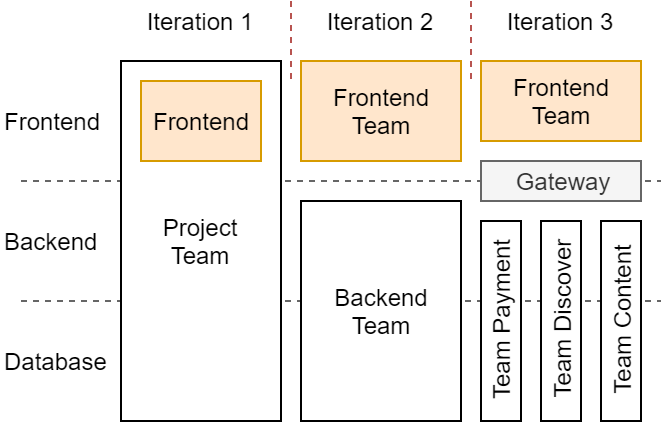
\includegraphics[scale=0.5]{evolution.png}
    \caption{Evolution of web architecture from the monolithic approach over frontend backend separation up to the microservices approach \cite[p.~17]{Wenzel.2020}}
    \label{img:evolution_of_web_architecture}
\end{figure}

These advantages resulted in a high rate of adoption of microservice architecture \cite{McCall.2019}, but it has downsides as well.
As shown in Figure \ref{img:evolution_of_web_architecture}, the server part is clearly separated into subdomains, whereas the frontend is still one big application.
The main intent of microservices is autonomy between teams, however, on the frontend side everything is  merged into one large project again, which can become a bottleneck for some projects \cite[p.~18]{Wenzel.2020}.
As a result, the mentioned benefits from the microservices architecture are lost in the frontend \cite{Leitner.2020}. %min 8:16
Consequently, the same idea of autonomy from the backend was introduced into the frontend with the \ac{MFA}, visualized in Figure \ref{img:micro_frontends_approach_detail} \cite{Geers.2019}.

Figure \ref{img:micro_frontends_approach_detail} uses the domain example shown in Figure \ref{img:evolution_of_web_architecture} and splits the frontend up.
As a result, there are independent teams which are responsible for one subdomain.
A subdomain contains all responsibilities from the frontend, over the backend and up to the database.
Consequently, it fully embraces the idea of autonomy from end to end \cite[p.18f.]{Wenzel.2020}.

\begin{figure}[h]
    \centering
    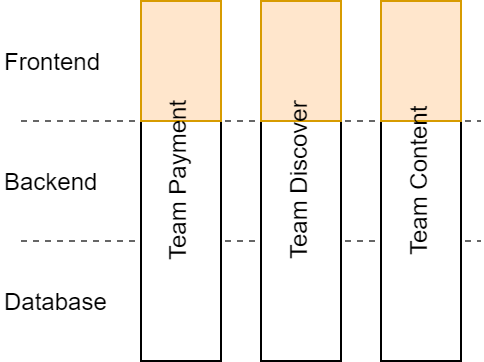
\includegraphics[scale=0.5]{mfa.png}
    \caption{Micro frontend architecture example with three teams \cite[p.~19]{Wenzel.2020}}
    \label{img:micro_frontends_approach_detail}
\end{figure}





\section{Micro frontend integration concepts}\label{cha:theory:concepts}

After explaining the origin of \acp{MF}, it is important to outline what \acp{MF} are, because there are several integration concepts.
The simplest concept is the \textit{Hyperlink integration}.
This concept utilizes hyperlinks to connect individual web pages (in this case \acp{MF}).
The advantage is that the interface surface is slim with a small complexity overhead.
However, there are disadvantages such as that only one \ac{MF} per page is allowed, transitions between \acp{MF} require roundtrips to the server and that the intercommunication between \acp{MF} is limited.
As a result, Hyperlink integration only works on a coarse grained level \cite{Leitner.2020}.
It is limited, because the only connection between the \acp{MF} is the \ac{URL}.
Hence, communication is limited to string serialized data.
Two options to transfer more complex information is via Server-Sent Events or a WebSocket connection.
Both require the backend to communicate instead \cite{Vogel.2020.Steyer}.

Concluding the \textit{Hyperlink integration}, the question remains whether the benefits mentioned beforehand in section \ref{cha:theory_evolution} are fulfilled.

\begin{itemize}
    \item Each \ac{MF} can be deployed independently from the other \acp{MF}
    \item If one \ac{MF} fails, others can continue working
    \item Each \ac{MF} can be built with a different stack
    \item Only a hyperlink connects the applications, which is the smallest interface surface possible
    \item Each \ac{MF} can be responsible for one business domain
    \item The \acp{MF} can be developed in parallel
\end{itemize}

Therefore, all benefits are met, which is also shown in the Table \ref{tbl:overview_concept_benefits} \cite{Leitner.2020}.

Besides \textit{Hyperlink integration}, there are also \textit{Build-Time integration}, \textit{Server-Side integration}, and \textit{Client-Side integration}.
These require a shell application which is responsible for integration.
Their difference lies in the time of integration \cite{Leitner.2020}.
In Figure \ref{img:container_application_concepts} the time differences are visualized.

\begin{figure}[h]
    \centering
    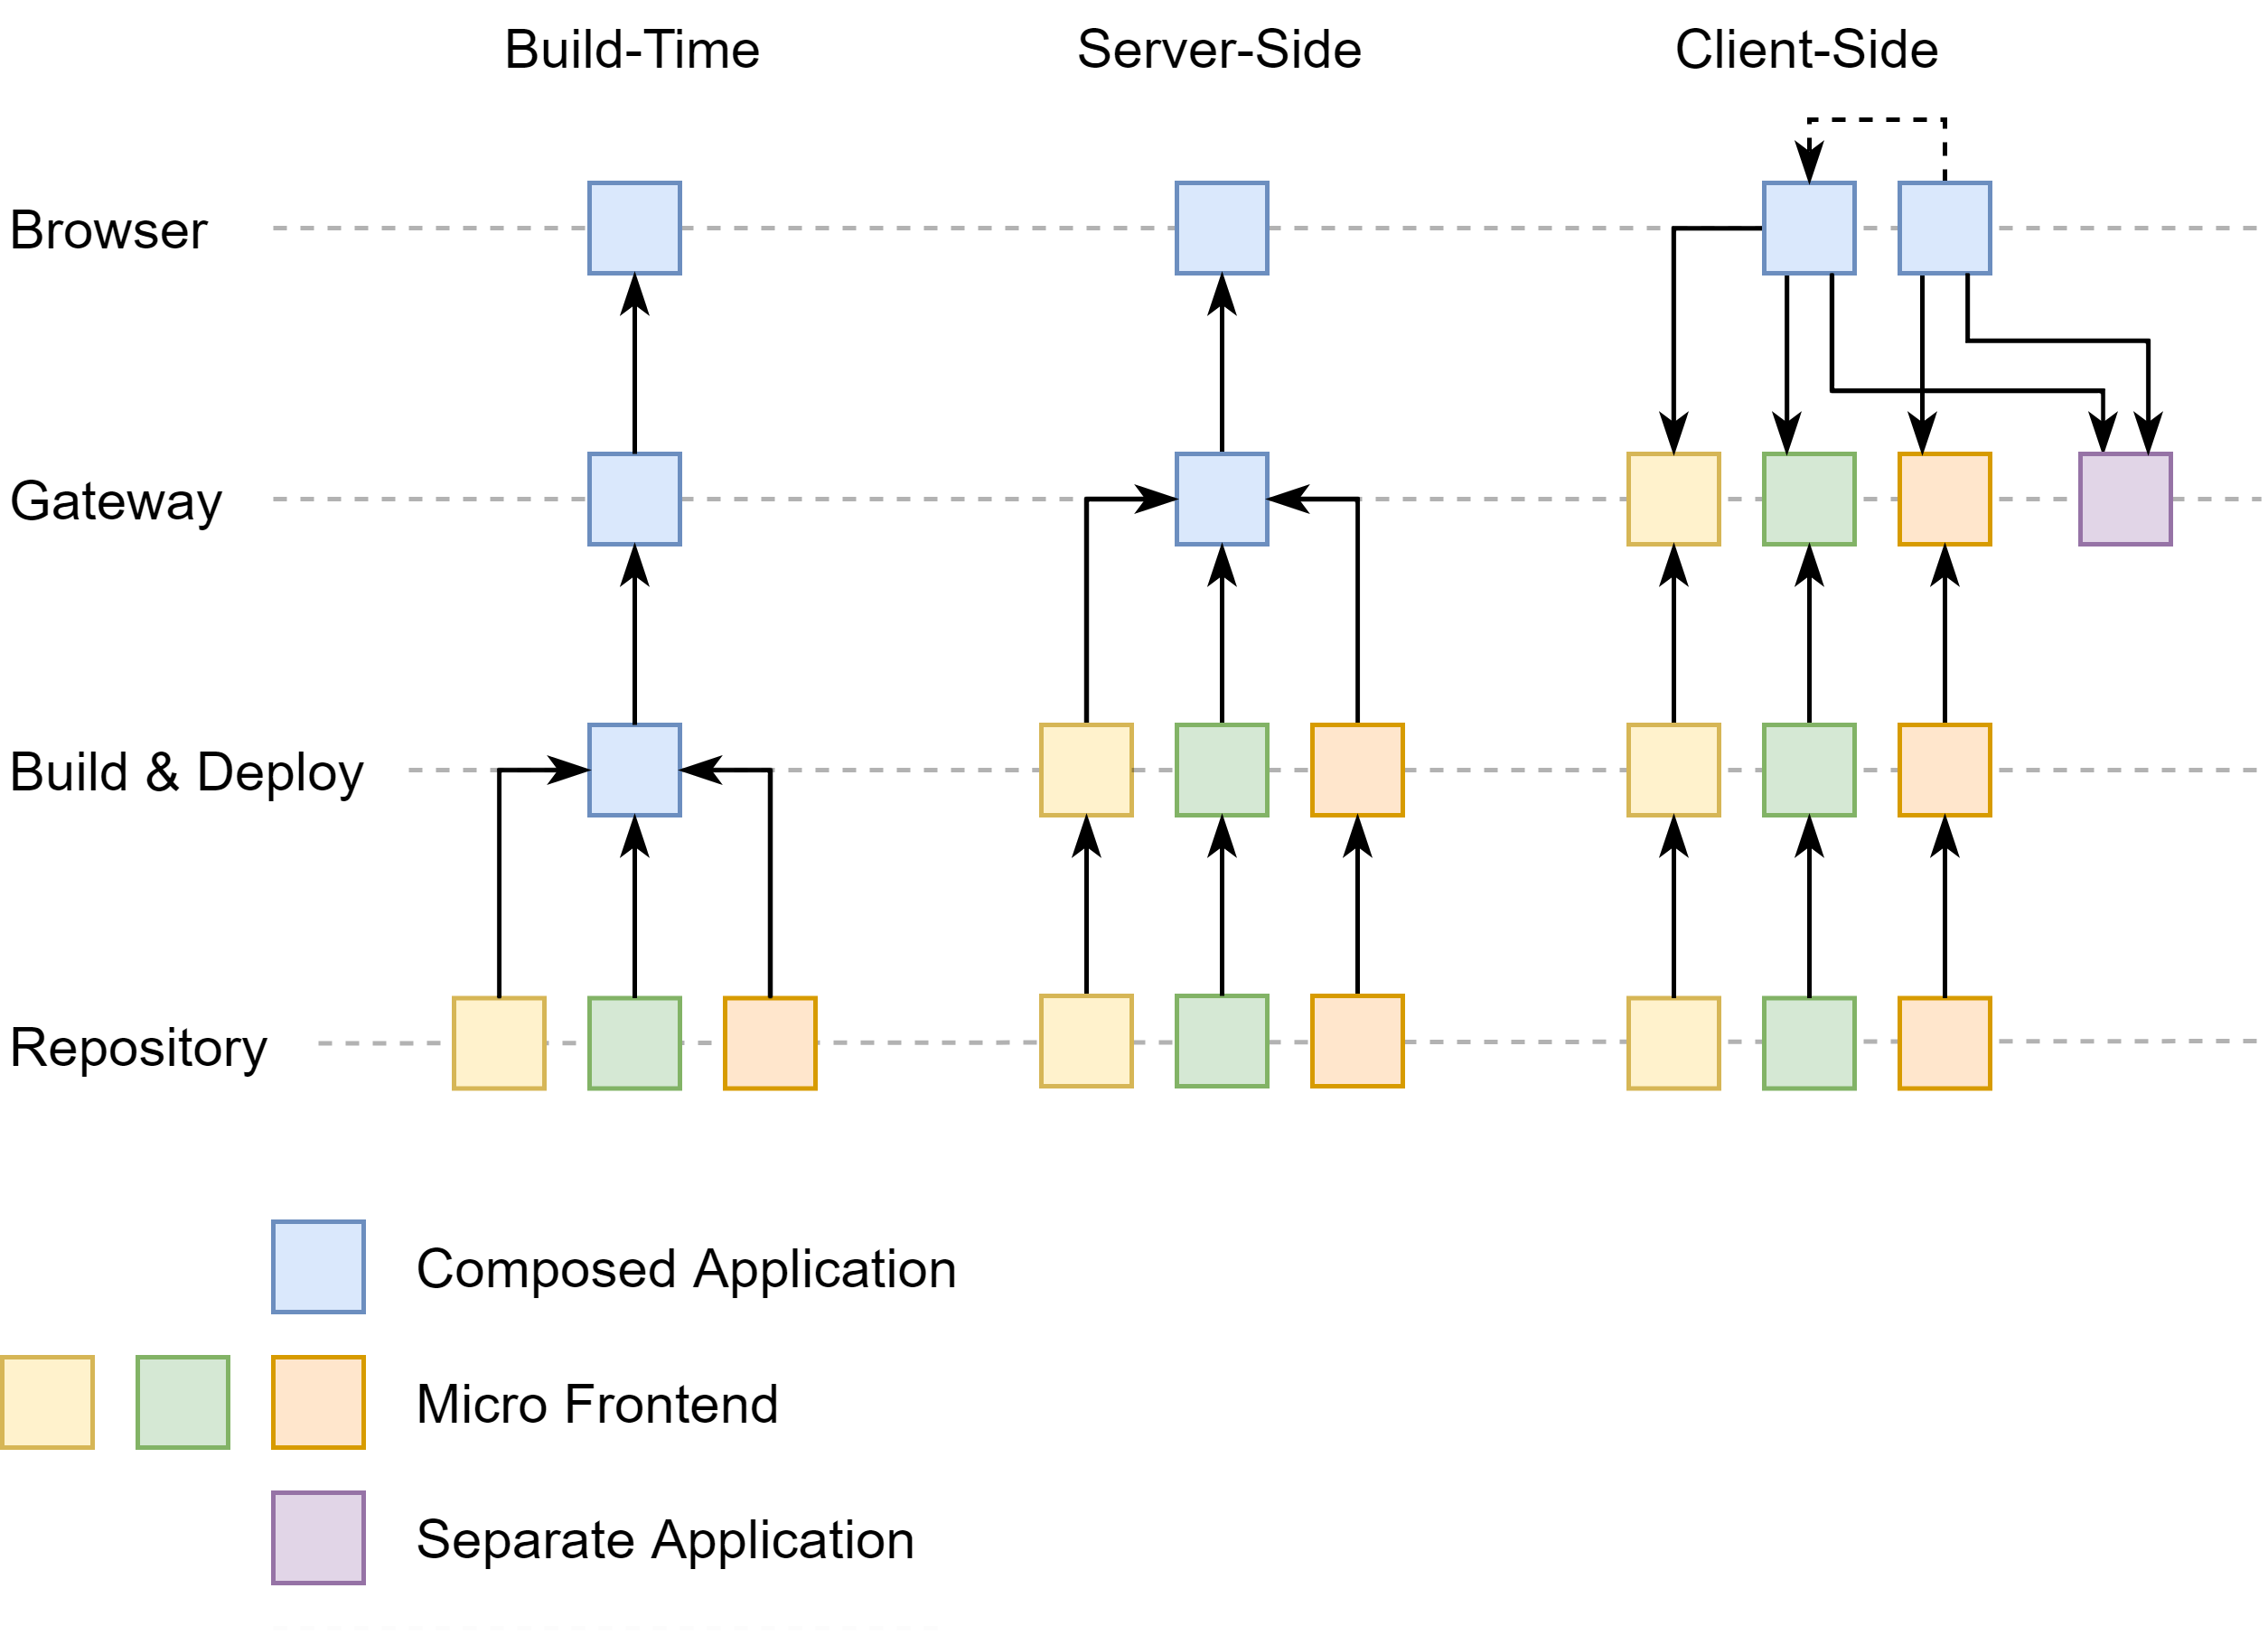
\includegraphics[width=\textwidth, keepaspectratio]{integration.png}
    \caption{Different shell application integration concepts in comparison to each other \cite{Leitner.2020}}
    \label{img:container_application_concepts}
    %min 22:50
\end{figure}

The first concept is \textit{Build-Time integration} and it is the earliest integration.
Each \ac{MF} is developed on their own, but they are combined to one application while building the application.
As a result, if any \ac{MF} is changed, then the entire application needs to be redeployed.
Hence, there is no independent deployment.
Another benefit which is missing is distinct operations.
It is very likely, that the entire application breaks if one \ac{MF} breaks.
Finally, the \acp{MF} needs to use the same technology stack in order to be built together into one application.

On the other hand, the \textit{Build-Time integration} concept allows for a small interface surface by dividing the application into separate components and \acp{MF}.
This concept also includes modeling around business domains and parallel development.
A comparison of the benefits to other concepts is shown in Table \ref{tbl:overview_concept_benefits} \cite{Leitner.2020}.

The next concept is \textit{Server-Side integration}.
Its main difference is, that each \ac{MF} is developed, built and deployed on their own and then connected before it leaves the server.
A typical approach is to use Edge-Side Includes to compose the final web page together in the gateway (i.e. the \enquote{edge}).
Contrary to the \textit{Build-Time integration}, each \ac{MF} is independent deployable.
Similarly are the distinct operations, because there are fallback solutions, if a Edge-Side Include is not available.
Also, because the composition part is about stitching together \ac{HTML} pieces, the \acp{MF} are technology agnostic.
Apart from these benefits, the other benefits apply as well, which are a small interface surface, being able to model around business domains and parallel development.
This is also shown in the Table \ref{tbl:overview_concept_benefits}.
The only disadvantage is, that it requires a lot of roundtrips to the server.
This also breaks an Single-Page Application concept.
Depending on the project this aspect can be a disadvantage or not.
It has the benefit of slim client-side applications, because less \ac{JS} is needed to compose the application client-side \cite{Leitner.2020}.

Finally, there is the \textit{Client-Side integration} concept, which is the relevant concept for this thesis.
It follows the same principles of the \textit{Server-Side integration}, but moves the integration into the client-side.
This results in also providing all benefits, which is shown in Table \ref{tbl:overview_concept_benefits}.
For this concept, a shell application is firstly loaded into the browser.
The shell is then responsible to load the needed \acp{MF} per page and integrate them.
Because the shell loads what it needs, the arrows are inverted in the Figure \ref{img:container_application_concepts} for the last step between the browser and gateway.
Also, each \ac{URL} is composed of different \acp{MF}, which results in multiple potential combinations.
This is outlined in the Figure by showing multiple \textit{Composed Applications} in the browser, which are connected via an arrow, representing the routing between them.
The final difference is, that this concept allows to integrate third-party applications.
This is hinted in the Figure by the \textit{Separate Application} which is integrated in the composed application.

\begin{table}[h]
    \begin{tabular}{|l|l|l|l|l|}
        \hline
                             &
        \textbf{Hyperlink}   &
        \textbf{Build-time}  &
        \textbf{Server-side} &
        \textbf{Client-side}
        \\ \hline
        \makecell[l]{Independent                                         \\ deployment}   & \cmark{} & \xmark{} & \cmark{} & \cmark{} \\ \hline
        Distinct operations  & \cmark{} & \xmark{} & \cmark{} & \cmark{} \\ \hline
        Technology agnostic  & \cmark{} & \xmark{} & \cmark{} & \cmark{} \\ \hline
        \makecell[l]{Small interface                                     \\ surface}& \cmark{} & \cmark{} & \cmark{} & \cmark{} \\ \hline
        \makecell[l]{Model around                                        \\ business domains} & \cmark{} & \cmark{} & \cmark{} & \cmark{} \\ \hline
        Parallel development & \cmark{} & \cmark{} & \cmark{} & \cmark{} \\ \hline
    \end{tabular}
    \caption{Overview of benefits per integration concept \cite{Leitner.2020}}
    \label{tbl:overview_concept_benefits}
\end{table}

To sum up this section, there are several approaches available to realize \ac{MFA}.
\textit{Hyperlink integration} is the simplest approach, but it is only suited for applications with fully verticalized systems.
Next up is \textit{Build-Time integration}.
Even though it does not provide all benefits, it can be a pre \ac{MFA} step in development \cite{Vogel.2020.Olleck}.
Finally, there are \textit{Server-Side integration} and \textit{Client-Side integration}.
Both provide all benefits and it comes down to the project needs, which concept is used in the end.
A final thought is not about the \ac{MFA}, but rather the fact that all these benefits come at the cost of complexity.
Each benefit mentioned comes with a complexity cost and it depends on a project which benefits are actually worth the cost.
This was mentioned by \textcite{Leitner.2020} and \textcite{Jackson.2019}.





\section{Micro frontend conceptual extensions}

After explaining the general integration concepts, there are also extensions to them which can be used if needed.
It is important to note, that from here on the practices are explained in context of \textit{Client-Side integration}.



\paragraph{\acl{BFF}}\label{cha:theory_extensions_bff}

The first conceptual extension is the architecture \acf{BFF} from the microservices architecture pool.
Normally this is used to reduce the responsibility of the \textit{\ac{API} gateway} in case that there are multiple client applications using the same backend.
To achieve the responsibility reduction, instead of using one \ac{API} gateway for all applications, it is split so that each client application uses a different \ac{API} gateway \cite[p.~69f.]{Bruce.2019}.
But before applying the \ac{BFF} to the \ac{MFA}, it is essential to outline the scenario without it.

\begin{figure}[h]
    \centering
    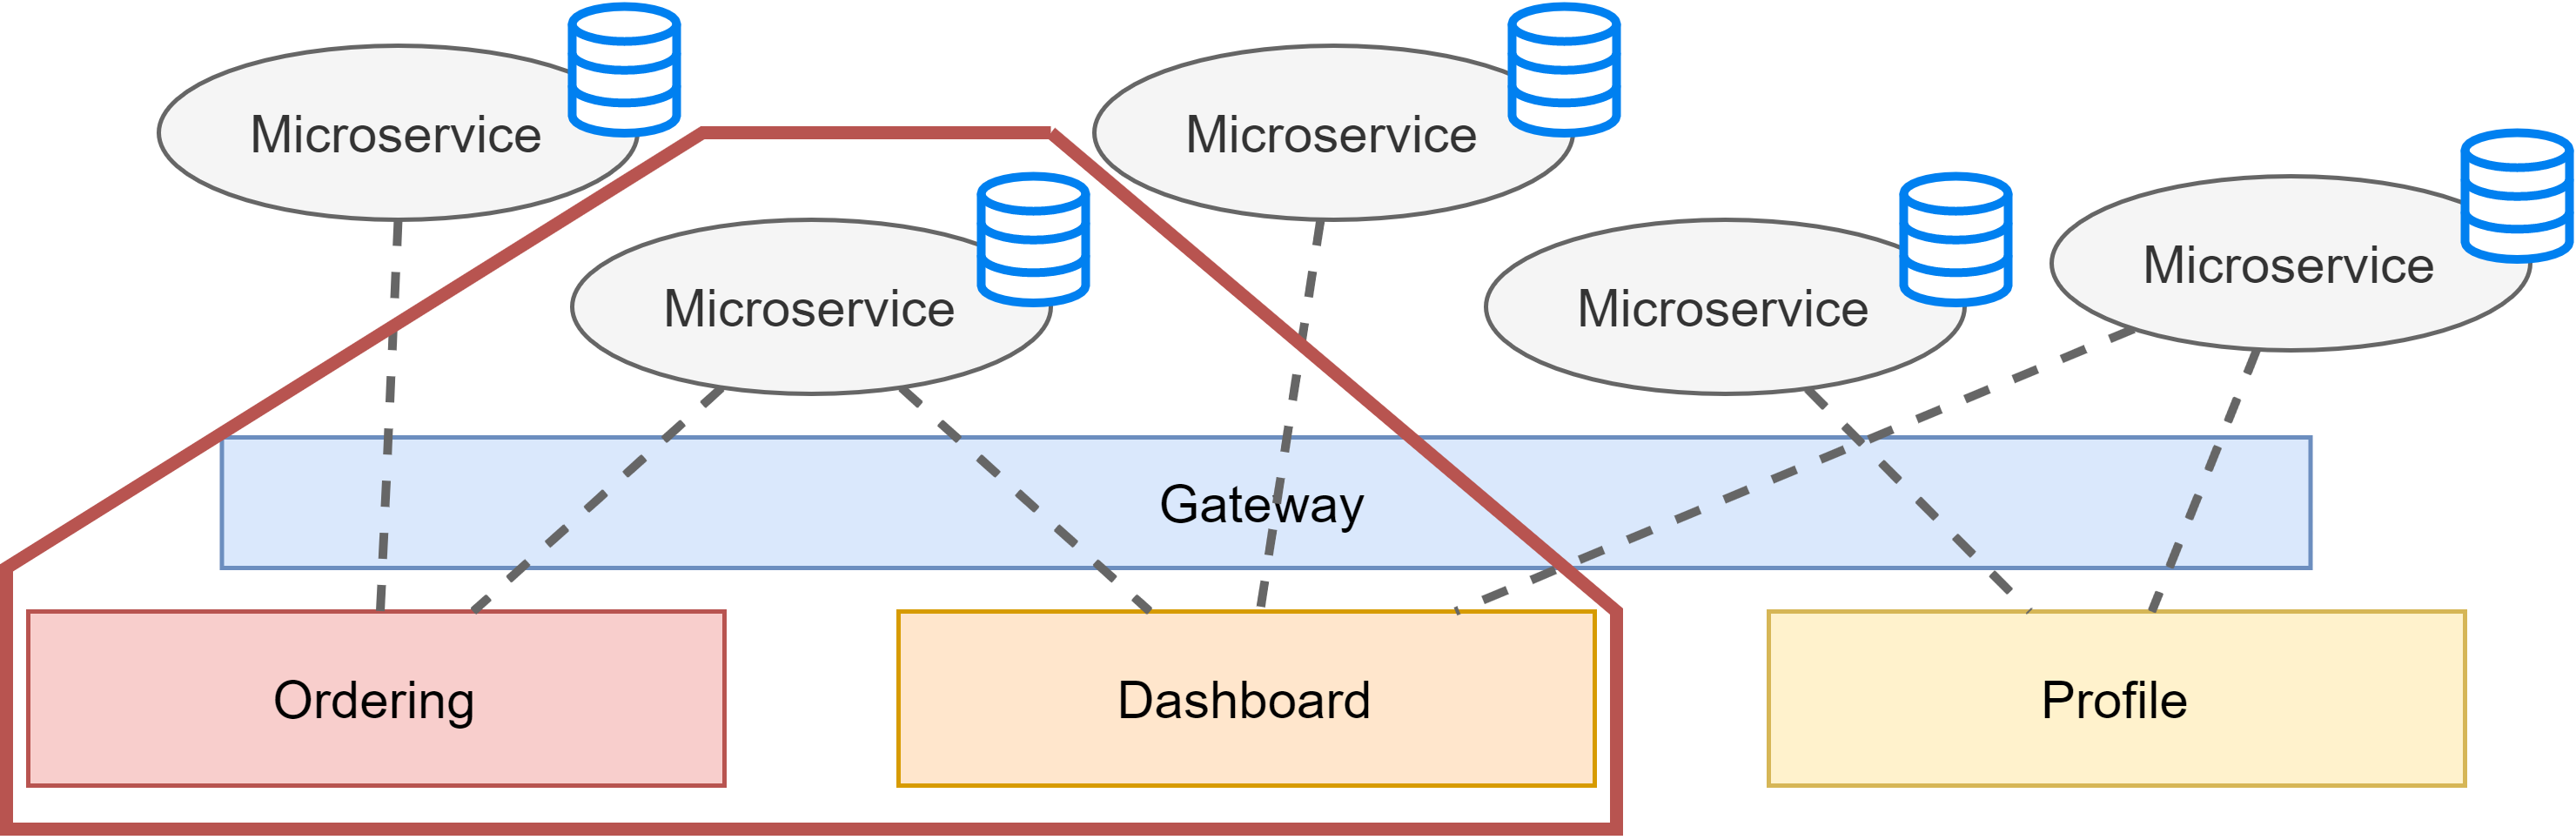
\includegraphics[width=\textwidth, keepaspectratio]{no-bff.png}
    \caption{Outline the coupling between \ac{MF}, if \ac{BFF} pattern is not used \cite{Leitner.2020}}
    \label{img:team_slicing_no_bff}
\end{figure}

The scenario shown in Figure \ref{img:team_slicing_no_bff} is, that one microservice is used by multiple \acp{MF}.
One instance is outlined in Red.
Assuming the microservice provides a service via some form over a gateway, both \acp{MF} will break, when the \ac{API} changes.
Hence, this creates an unwanted coupling between \textit{Ordering}, \textit{Dashboard} and the microservice.
As a result, the autonomy aspect between these parties is broken.

Before explaining how to fix the problem, first is important how the \ac{BFF} pattern can be translated to work with \ac{MFA}.
This is shown in Figure \ref{img:team_slicing_bff}.
Each \ac{MF} gets its own microservice and it is the only communication channel from the \ac{MF} to the backend.
Therefore, the \ac{BFF} microservice provides the \ac{API} for the \ac{MF} and handles all the communication with multiple microservices.
As a result, the \ac{MF} and \ac{BFF} microservice is considered to be one unit and the same team must be responsible for both \cite{Leitner.2020}.

\begin{figure}[h]
    \centering
    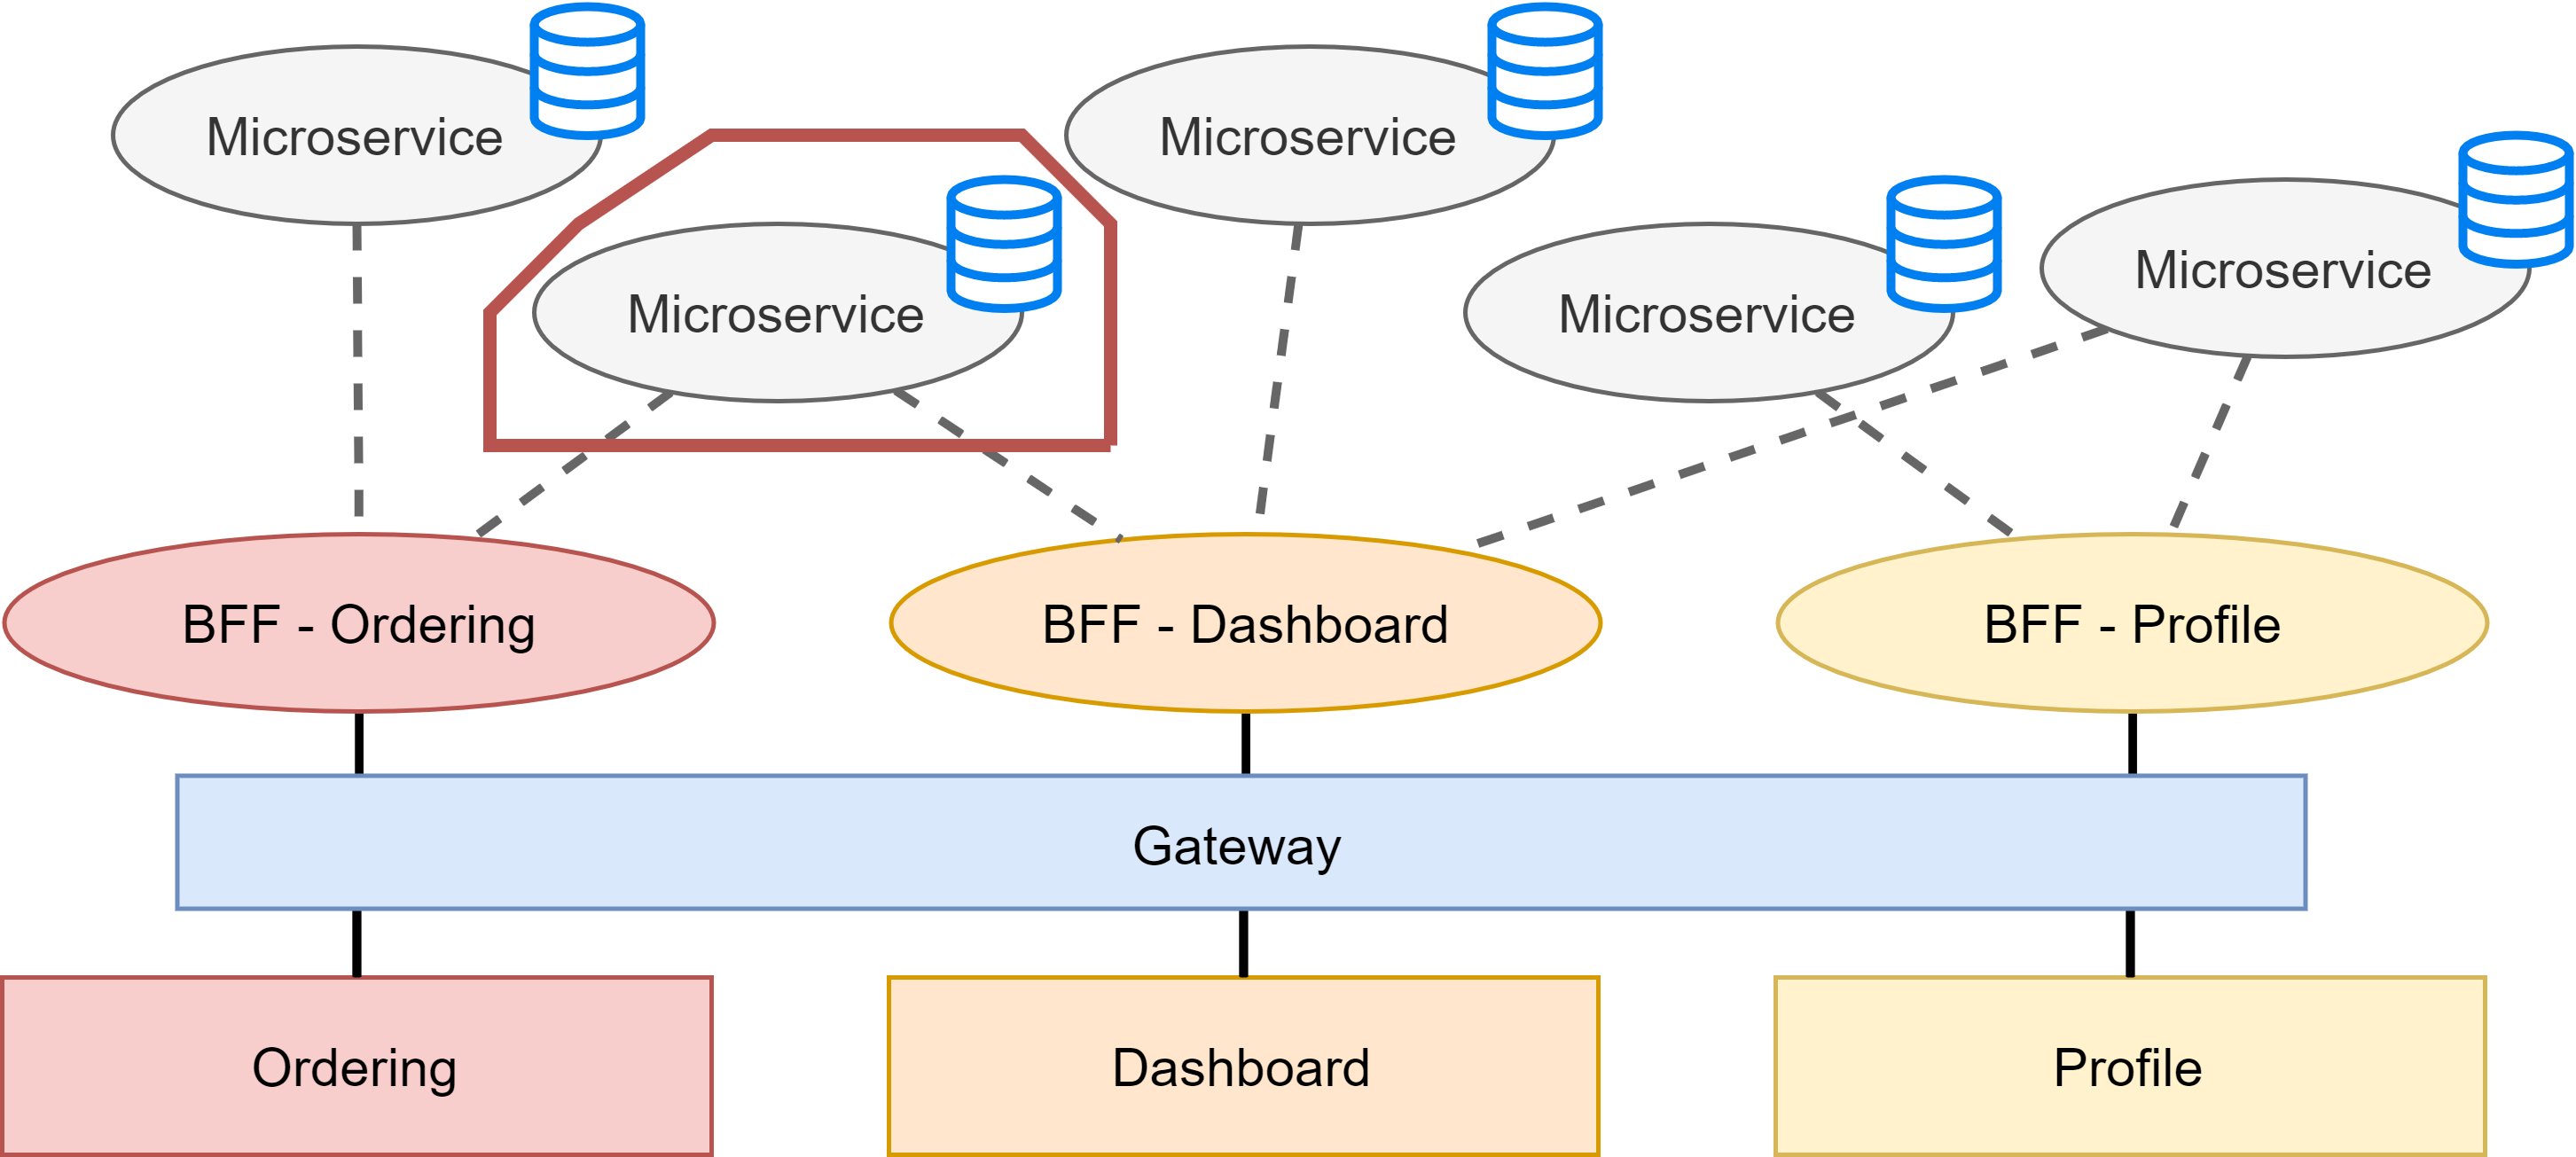
\includegraphics[width=\textwidth, keepaspectratio]{bff.png}
    \caption{Using the \ac{BFF} architecture in combination with the \ac{MFA} \cite{Leitner.2020}}
    \label{img:team_slicing_bff}
\end{figure}

The coupling problem is solved with the \ac{BFF} pattern, because there is a clear responsibility cut between the \ac{MF} and its \ac{BFF} micro frontends to the shared microservice.
This approach was mentioned by \textcite{Jackson.2019}, \textcite{Leitner.2020} and \textciteRehm{}.

There are different interpretations on how much responsibility the dedicated microservice should have.
\textcite{Leitner.2020} suggests that it is only used to accumulate and provide information for the \ac{MF}.
By contrast, \textcite{Jackson.2019} does not restrict the responsibility of the dedicated microservice.
However, both agree that one team should be responsible for the micro frontend and its dedicated microservice.

Using the \ac{BFF} architecture is not required in order to use \acp{MF}, instead it is an extension and has both advantages and disadvantages.
An important advantage is that it simplifies sharing microservices between multiple \acp{MF} without creating unwanted coupling between \acp{MF} and microservices.
However, adding a new microservice adds complexity to the overall system.



\paragraph{Micro frontend composition}\label{cha:theroy_extensions_composition}

Another aspect to outline about \ac{MFA} is the composition part.
Three approaches are commonly outlined, which are shown in Figure \ref{img:compositions}.
The first one is to show one \ac{MF} per page (left).
This is considered as the default approach and is the simplest approach compared to the other approaches.
Next is to show multiple \acp{MF} per page (middle).
In this case, each \ac{MF} is placed into its own node and there is a clear boundary between them.
This requires some form of templating, which is addressed in the \textit{\nameref{cha:requirement_detail_integration_pagelayout}} requirement.
Finally, the widget approach can be seen at the right.
It allows each \ac{MF} to share components with other \acp{MF} and they can be included by \acp{MF} as needed.
How to implement it is discussed in the \textit{\nameref{cha:requirement_detail_integration_widget}} requirement.
One combination that was not mentioned in the literature research, is to combine widgets and multiple \acp{MF} per page.
Although this is possible, no practical scenario is mentioned where it is needed.

\begin{figure}[h]
    \centering
    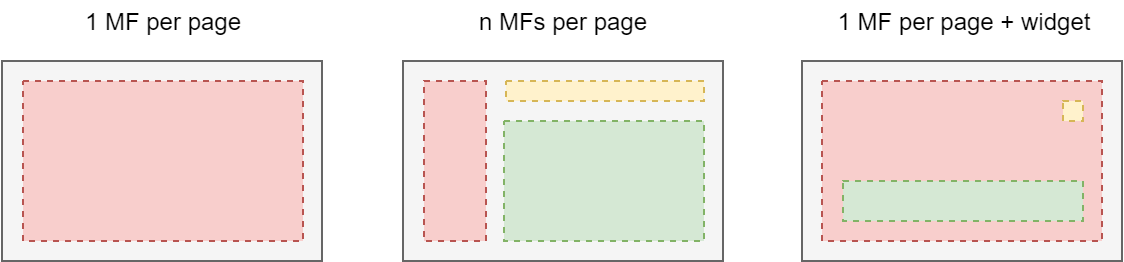
\includegraphics[width=\textwidth, keepaspectratio]{compositions.png}
    \caption{Different \ac{MF} composition approaches}
    \label{img:compositions}
\end{figure}



\section{Micro frontend practical parts}\label{cha:theory_practic}

Before concluding the \ac{MF} fundamentals, there are some topics worth mentioning, because they come up in the chapter \ref{cha:requirement}.



\paragraph{Bundle size}

A term used multiple times in the chapter \ref{cha:requirement} is bundle size.
It refers to the entire size of the application's \ac{JS} bundle.
It is relevant, because a \ac{MF} application consists of many \ac{MF} and each is bundled separately.
This can result in a lot of data which is required for the application.



\paragraph{Duplicate requrests}

As shown in the \nameref{cha:theory_extensions_bff} paragraph, \acp{MF} should be independent and there are scenarios where two \acp{MF} need data from the same microservice.
If the implementation strongly follows the concept of \ac{MFA}, then each \ac{MF} fetches the data on their own.
However, this can result in a poor \ac{UX}.
Therefore, there are approaches which tackle this issue, with the expense of autonomy.
This is mainly addressed in the \hyperref[cha:requirement_detail_performance]{Performance} requirement \cite{Steyer.2019}.



\paragraph{Custom Events}\label{cha:theory_practice_customevents}

Custom Events is a browser native feature to emit events on a node in the \ac{DOM} and listen for them.
A Custom Event consists of a name and any data which is added to it.
To emit it, a \ac{HTML} element is needed as host.
Any \ac{JS} code can listen on any \ac{HTML} element for events which are emitted on this particular element\footnotemark.
\footnotetext{\url{https://developer.mozilla.org/en-US/docs/Web/Guide/Events/Creating_and_triggering_events} (Visited on 09/02/2020)}



\paragraph{\acl{CDC} testing}\label{cha:theory_practice_cdctesting}

\ac{CDC} testing is about abstracting the communication between two parties to test them in isolation of each other.
This implies, that only one of both is needed in order to test the communication at a time.
Hence, each party is responsible to validate these tests before deployment to ensure that a build is working according to the contract.
A contract is either created by hand or via a tool\footnotemark.
\footnotetext{\url{https://www.martinfowler.com/articles/consumerDrivenContracts.html} (Visited on 02/09/2020)}
A common tool for such tests in a microservice environment was mentioned by \textcite{Laug.2018}, which is \textit{pact.io}.
This tool simplifies the automation process of such tests.



\paragraph{Web Components}\label{cha:theory_practice_webcomponent}

Web Components is a native browser feature which consists of \textit{Custom elements}, \textit{Shadow \ac{DOM}} and \textit{\ac{HTML} templates}.
\textit{Custom elements} is a \ac{JS} \ac{API} to create reusable custom components and define their behavior for a web page.
Such a \textit{Custom element} requires a tag name, which must include a dash by convention.
A tag name can only exist once per page\footnotemark{}.
\footnotetext{\url{https://developer.mozilla.org/en-US/docs/Web/Web_Components} (Visited on 09/02/2020)}
Furthermore, the \textit{Custom element} \ac{JS} \ac{API} provides the ability to either pass information into the custom element via \ac{HTML} attributes or \ac{JS} properties.
The first can be achieved by adding the attribute into the custom element tag in the \ac{HTML}.
Contrary to that, the latter needs \ac{JS} to retrieve the custom component node from the \ac{DOM} in order to access its properties via methods from the custom component\footnotemark.
\footnotetext{\url{https://developers.google.com/web/fundamentals/web-components/customelements\#properties_and_attributes} (Visited on 09/02/2020)}

An optional feature of a \textit{Custom element} is the \textit{Shadow \ac{DOM}}.
The \textit{Shadow \ac{DOM}} is a \ac{JS} \ac{API} to attach a virtual \ac{DOM} to the actual \ac{DOM}, hence the name \textit{shadow}.
These elements are rendered separately from the actual \ac{DOM}.
It also allows to encapsulate \ac{CSS} styles within itself.
As a result, the main page is only able to style the \ac{CSS} via variables, while the styles from within the \textit{Shadow \ac{DOM}} do not affect the main page\footnotemark{}.
\footnotetext{\url{https://developers.google.com/web/fundamentals/web-components/shadowdom\#stylefromoutside} (Visited on 09/02/2020)}

Lastly, there are \textit{\ac{HTML} templates}, which provide the \textit{template} and \textit{slot} tag.
Only the \textit{slot} tag is required later on in chapter \ref{cha:requirement}.
It is a placeholder within the Web Component that can be filled with any markup from within the main page\footnotemark.
\footnotetext{\url{https://developer.mozilla.org/en-US/docs/Web/HTML/Element/slot} (Visited on 09/02/2020)}





\section{Conclusion}

To conclude the \ac{MF} fundamentals, there are some important hints about \acp{MF} in general.
The first is from \textcite{Laug.2018b} who points out, that \ac{MFA} does not increase the development speed, but rather sustains it.
He mentions, that this is a common misconception of the micro architectures.
Secondly, \textcite{Leitner.2020} believes that no more than 20\% of projects actually need the \ac{MFA}.
He continues, that the \ac{MFA} adds a lot of complexity, which must be worth it for the project in order to use \ac{MFA}.
Finally, \textcite{Steyer.2019} came up with a simple decision tree to find out if a project even needs this architecture, which is shown in Figure \ref{img:decision_tree}.
The tree starts on the left side and, based on it, only in a specific case the architecture is recommended.
More about the criteria for a \ac{MF} application is described in section \ref{cha:scenarios_criteria}.

\begin{figure}[h]
    \centering
    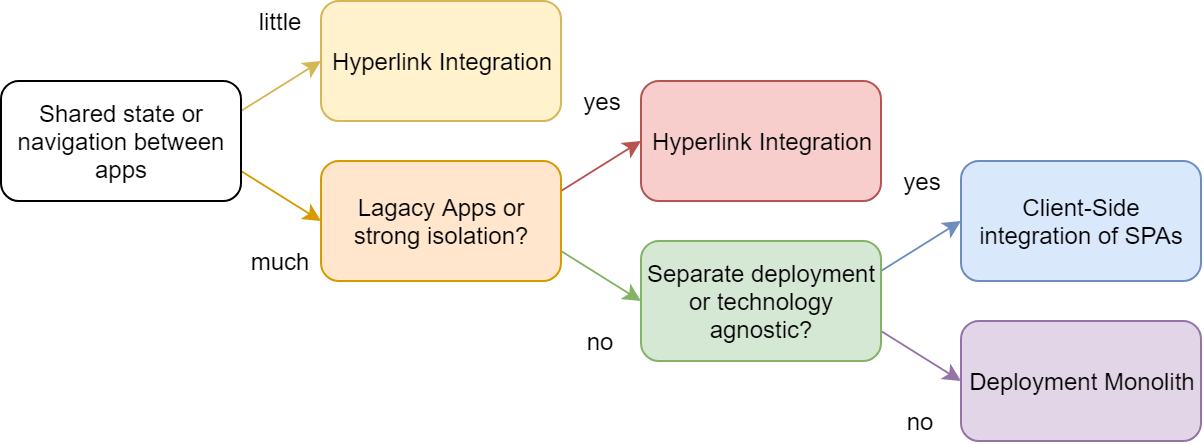
\includegraphics[width=\textwidth, keepaspectratio]{decition_tree.png}
    \caption{Decision tree from \ac{MFA} which can be used to determine which type of architecture or implementation should be used \cite{Steyer.2019}}
    \label{img:decision_tree}
\end{figure}

This sums up the \ac{MF} fundamentals chapter and the next chapter is about when to use the \ac{MFA}.




% Requirement Analysis
%!TEX root = ../documentation.tex

\chapter{Application scenarios}\label{cha:scenarios}

One aspect while researching the \ac{MFA} became apparent, namely that it is relevant to consider that requirements change depending on the application scenario.
There are several requirements for \ac{MF} applications, and it is not apparent which requirements are needed or useful for any given application.
Therefore, the intent of the second question in the expert  interviews (see \ref{cha:appendix_expertinterview_questions}) is to collect information on different \ac{MF} application scenarios and connect the information with requirements.
Initially, the intent of the second question was to gain intel about real world examples and later link the examples to requirements.
The goal was to provide in-depth information of which requirement is needed for which kind of application.
Therefore, the experts should name suitable scenarios for the \ac{MFA}.
But all experts believe that it can not be pinpointed to scenarios, but rather criteria.
As a result, the experts' information for the first question are summarized in \ref{cha:scenarios_types} and the named criteria are summarized in \ref{cha:scenarios_criteria}.





\section{General application types for micro frontend architecture}\label{cha:scenarios_types}

Based on the expert interviews and conference presentations, three general application types have been identified where \ac{MFA} can be used.
These general types are collections of statements.



\paragraph{Enterprise Application}\label{cha:scenarios_enterprise}

The first application type is an \nameref{cha:scenarios_enterprise}.
Generally this application type is used company-internal and the devices for access are typically known or at least the minimum performance is known.
Therefore, they can be device specific and do not necessarily support multiple platforms.
This narrows the supported device scope and hence more platform specific approaches can be used.
Furthermore, such an application is likely to be used frequently or it is at least accessed via a fast and stable internet connection, like for example a \ac{LAN} connection.
As a result an extensive caching approach is recommendable and the application size is not as relevant as in the other application types.
Another aspect is that multiple companies could work on the same application, which requires enforcing autonomy of the teams.
In the end, such an application can have a user base ranging from a few experts to an enterprise-wide tool with 15.000 or more users.
This type of application was mostly named by experts and in conference presentations, namely by \textcite{Laug.2018}, \textciteRehm{}, \textciteHuber{}, \textciteSteyer{} and \textciteOlleck{}.



\paragraph{Consumer Application}\label{cha:scenarios_consumer}

The second application type is the \nameref{cha:scenarios_consumer}.
Other than the \nameref{cha:scenarios_enterprise}, this application type is used from any kind of network or device.
Moreover, it is to be expected that these devices or networks are slow.
As a result, performance aspects like application size and request amount to the backend are important to ensure a good \ac{UX}.
In the expert interview with \textciteJovanovic{}, he pointed out that performance is the most critical requirement for these applications.
Also, the application probably has a varying active user base, which means that caching is only effective for the active user base.
Depending on the application, it could even be used from a smart TVs for instance.
\textciteMezzalira{} pointed out, that the browsers in such devices support less features than a regular desktop or mobile browser.
For example Web Components are currently not supported.



\paragraph{Off-the-shelf Application}\label{cha:scenarios_offshelf}

An \nameref{cha:scenarios_offshelf} is a product from a company which is distributed and customized for customers.
It is similar to an \nameref{cha:scenarios_enterprise}, but due to the customization requirement it has a slightly shifted focus.
For example, the application needs to be extendable via custom build features from the customer or even third-party companies.
To enable such behavior, the application probably needs to provide an interface for these features.
Another fact which changes from the \nameref{cha:scenarios_enterprise} is that the performance of the user devices is probably not known.
Therefore, it is important to invest into performance to ensure a good \ac{UX} for the customers \cite{Grijzen.2019}.
As a result, this application type can be placed between \nameref{cha:scenarios_enterprise} and \nameref{cha:scenarios_consumer}.





\section{Typical criteria to consider micro frontend architectures}\label{cha:scenarios_criteria}

After describing the general application types, the experts also pointed out which criteria needs to apply to at least consider a \ac{MFA}.
The criteria mostly mentioned is a large team size.
It was named by \textciteRehm{}, \textciteOlleck{}, \textciteJovanovic{} and \textciteMezzalira{}.
\citeauthorMezzalira{} provides more detail by indicating that at least 50 developers should work on the application.

Another criterion is bound to the project or team structure.
If a project is developed in an agile environment, follows the DevOps culture, or has cross-functional teams in general, then using the \ac{MFA} could maintain the development speed.
This was pointed out by \textciteRehm{}.
\textciteJovanovic{} suggested that the \ac{MFA} should be used if it suits the organization.
This includes the named structures, but possibly also other practices like \textit{Extreme Programming}.
The next criteria named by \textciteOlleck{} is, that the project consists of strongly separated business functionalities.

Consequently, he points out that enforcing the strong separation with the \ac{MFA} will most likely maintain development speed over time.
Besides that, \textciteOlleck{} and \textciteJovanovic{} mention that a big application is also a criteria.
Moreover, \citeauthorOlleck{} mentioned the criteria, that if multiple companies work on the same project, the \ac{MFA} will reduce the communication needed between these companies making an independent deployment simpler.
Lastly, an \nameref{cha:scenarios_enterprise} is well suited for the \ac{MFA}.
\textciteSteyer{} points out, that the micro-architecture trend also started with \nameref{cha:scenarios_enterprise}s, which started to implement the microservice architecture first.

Another criterion or rather scenario is gradually converting from a monolith to a \ac{MF} application.
\textciteSteyer{} mentioned that it is not a common scenario, while \textciteJovanovic{} worked on such a project and \textcite{Jackson.2019} also supports the idea.
Hence, this scenario can be considered as a criterion for considering the \ac{MFA}.
Finally, \citeauthorSteyer{} experienced that nearly all \ac{MF} applications were green field projects, which he supervised.
A green field project is a project which starts from scratch, therefore the term \enquote{green field}, because there is nothing implemented yet.

To sum up this chapter, there are three application types for \ac{MFA}, namely \textit{\nameref{cha:scenarios_enterprise}}, \textit{\nameref{cha:scenarios_consumer}} and \textit{\nameref{cha:scenarios_offshelf}}.
Still, they practically cover all applications.
Therefore, some criteria should be met in order to start considering using the architecture.

\begin{itemize}
    \item Large teams
    \item Suiting the project or organization structure
    \item Strongly separated business functionalities
    \item Application size
    \item Multiple companies working on the same application
\end{itemize}


% Requirement Analysis
%!TEX root = ../documentation.tex

\chapter{Application requirement analysis}\label{cha:requirement}

In order to evaluate if there is a need for a generalized shell application, it is important to first understand what the requirements for such an application are.
To get the needed insights a requirement analysis is conducted via literature research and the expert interviews.
This chapter focuses on outlining requirements and comparing them against each other.

The found requirements can be divided into categories.
These are explained in section \ref{cha:requirement_categories}.
After that, an overview of all requirements is provided in the section \ref{cha:requirements_overview}.
This includes an explanation on how the requirements were compared against each other in terms of importance, and an overview, seen in Table \ref{tbl:overview_requirements}, which contains all found requirements.
Following that are multiple sections which describe the requirements in detail (section \ref{cha:requirement_detail_integration}, \ref{cha:requirement_detail_performance}, \ref{cha:requirement_detail_state}, \ref{cha:requirement_detail_style} and \ref{cha:requirement_detail_developer}).
Lastly, a conclusion for this chapter is drawn in section \ref{cha:requirements_conclusion}.



%!TEX root = ../../documentation.tex

\section{Requirement categories}\label{cha:requirement_categories}

During the requirements research it became apparent that requirements can be divided into categories.
Grouping requirements by categories further structures the analysis.
This also allows to order them based on there importance.
Thus, the following list shows an interpretation of requirement categories and their importance in descending order.
Each category is abbreviated, except \textit{Performance}, as seen in the following list.
They are also used in the Table \ref{tbl:overview_requirements}.

\pagebreak

\begin{enumerate}
    \item Browser routing and integration approach \textit{(Integration)}
    \item Performance
    \item Shared state and micro frontend inter-communication techniques \textit{(State)}
          \begin{itemize}
              \item Internationalization
              \item Authentication
          \end{itemize}
    \item Styling handling \textit{(Style)}
    \item Developer experience \textit{(Developer)}
          \begin{itemize}
              \item Tools
              \item Debugging
              \item Testing
          \end{itemize}
\end{enumerate}

To challenge the interpretation, each expert was asked to validate it.
This was the third question of the expert interviews (see Appendix \ref{cha:appendix_expertinterview_questions}).
All experts agreed with the selected categories, but the order of importance was slightly different.
An overview of all opinions about the importance is shown in Table \ref{tbl:overview_requirements_categories}.
The number on the left indicates the score.

\begin{table}[h]
    \setlength{\tabcolsep}{4.265pt} % Default value: 6pt
    \begin{tabularx}{\linewidth}{|l|l|l|l|l|l|l|}
        \hline
        \textbf{S}                              &
        \textbf{LM} \cite{Vogel.2020.Mezzalira} &
        \textbf{PR} \cite{Vogel.2020.Rehm}      &
        \textbf{PH} \cite{Vogel.2020.Huber}     &
        \textbf{MS} \cite{Vogel.2020.Steyer}    &
        \textbf{BO} \cite{Vogel.2020.Olleck}    &
        \textbf{IJ} \cite{Vogel.2020.Jovanovic}
        \\ \hline
        1
                                                &
        Integration
                                                &
        Integration
                                                &
        Integration
                                                &
        Integration
                                                &
        Integration
                                                &
        Performance
        \\ \hline
        2
                                                &
        State
                                                &
        Performance
                                                &
        State
                                                &
        Performance
                                                &
        State
                                                &
        Integration
        \\ \hline
        3
                                                &
        Developer
                                                &
        State
                                                &
        Performance
                                                &
        State
                                                &
        Performance
                                                &
        State
        \\ \hline
        4
                                                &
        Performance
                                                &
        Style
                                                &
        Style
                                                &
        Style
                                                &
        Style
                                                &
        Style
        \\ \hline
        5
                                                &
        Style
                                                &
        Developer
                                                &
        Developer
                                                &
        Developer
                                                &
        Developer
                                                &
        Developer
        \\ \hline
    \end{tabularx}
    \caption{Overview of the different opinions about requirement categories}
    \label{tbl:overview_requirements_categories}
\end{table}

% score calculation explanation
In order to determine the order of importance based on the expert's opinion, a score is calculated.
Each position is weighted with a number equal to the order, which is the first column \textit{S}.
The most important is equal to 1, the second is equal to 2 and so on.
The final score of each category is determined by averaging all scores.
The results are shown in Table \ref{tbl:category_scores}.
In conclusion, \textit{Integration} is the most important category.
Following that is the \textit{Performance} and \textit{State} on second, followed by \textit{Style} and lastly \textit{Developer}.
The result is close to the initially predicted order of importance.

\begin{table}[h]
    \newcolumntype{s}[1]{>{\hsize=#1\hsize}X}
    \begin{tabularx}{\linewidth}{|X|X|X|X|X|}
        \hline
        \textbf{Integration} &
        \textbf{Performance} &
        \textbf{State}       &
        \textbf{Style}       &
        \textbf{Developer}
        \\ \hline
        $ \approx 1,2$
                             &
        $ \approx 2,5$
                             &
        $ \approx 2,5$
                             &
        $ \approx 4,2$
                             &
        $ \approx 4,7$
        \\ \hline
    \end{tabularx}
    \caption{Requirement categories scores based on expert opinions}
    \label{tbl:category_scores}
\end{table}


\section{Requirement analysis result overview}\label{cha:requirements_overview}

The analysis led to many requirements.
To better outline the importance of each requirement, they need to be scored in some way.
In order to achieve this, the process of the pairwise comparison technique is used.
This technique determines the relative importance by comparing requirements against each other and thus, obtaining a score for all requirements \cite[p.~573]{Achimugu.2014}.

The technique was modified in order to use it for the requirement analysis.
Instead of weighting the requirements, the expert statements are weighted based on the questions.
In the expert interviews, the questions four, five and six are used to gain insights into requirements and their approaches (see \ref{cha:appendix_expertinterview_questions}).
Each of the questions is assigned with a different weight.

\begin{itemize}
    \item Question four, \textit{What are requirements for the named shell application scenario which you had from a customer?}: They can be an any importance and thus, receive a score of 1
    \item Question five, \textit{Can you name any requirements which are needed for all shell application scenarios?}: These are the most important requirements in context of this thesis and thus, receive a score of 3
    \item Question six, \textit{What are the most difficult requirements to achieve and why?}: A general goal of architecture is to reduce the complexity of a project \cite[p.~98]{AlSharif.2004} and therefore, these requirements receive a score of 2
\end{itemize}

By introducing the score the focus can be shifted towards the relevant requirements.
Therefore, the requirements with a score of 5 or higher are considered relevant.
The reason is, that a low score makes it less likely that a requirement is actually needed.
It is important to note, that not all requirements can be part of a generalized shell application.
Hence, low scoring requirements are considered but they are a optional feature of the generalized shell application.


The requirements analysis was not only conducted via the expert interview, but also through a literature research.
Requirements found in the literature research receive a score of 1, because the context is not the same as in the expert interviews and therefore, comparability is not guaranteed \cite[p.~35]{AlexanderBognerBeateLittigWolfgangMenz.2009}.
On the other hand, requirements mentioned in literature should be considered as well to ensure a broad view.
Therefore, a score equivalent of question four in the interview is suitable.

After collecting the weights for each requirement, the weights are added up and resulting in the score.
In case of a score tie, the respective requirements are considered equally relevant.
Also, requirements are not only ordered by their score, but also by their respective category.
The categories are explained in the next section \ref{cha:requirement_categories}.

An overview of the requirement analysis result is shown in Table \ref{tbl:overview_requirements}.
In addition to this Table, there are two more tables in the appendix \ref{cha:appendix_requirements_overview}.
The first (\ref{tbl:adx_requirements_scores}) shows the score of each requirement and the second (\ref{tbl:adx_requirements_references}) shows which reference mentioned the requirement, considers it as difficult and as critical.
Further detail for the requirements will be provided in the following sections from  \ref{cha:requirement_detail_integration} to \ref{cha:requirement_detail_developer}.

%!TEX root = ../../documentation.tex

\setlength{\tabcolsep}{4.265pt} % Default value: 6pt
\begin{longtable}{|l|l|p{0.56\textwidth}|}
	% \begin{longtable}{ l l p{0.56\textwidth} }
	\hline
	\textbf{Category}             & \textbf{Requirement}   & \textbf{Description}                                                                               \\ \hline
	\multirow{12}{*}{Integration} & Loading                & Load a \ac{MF} into the application and provide it for further use                                 \\ \cline{2-3}
	                              & Lifecycle management   & A \ac{MF} can be bound and unbound to the \ac{DOM}                                                 \\ \cline{2-3}
	                              & Routing                & Enable page changes based on the \ac{URL} changes                                                  \\ \cline{2-3}
	                              & Configuration          & Behavior of \ac{MF} should be configurable                                                         \\ \cline{2-3}
	                              & Integration            & Compose a \ac{MF} into the current application                                                     \\ \cline{2-3}
	                              & Shared logic           & The shell provides logic for all \ac{MF}                                                           \\ \cline{2-3}
	                              & Widgets                & A \ac{MF} exposes a widget which can be used by an other \ac{MF}                                   \\ \cline{2-3}
	                              & Page layout            & The shell should control the page layout                                                           \\ \cline{2-3}
	                              & Indexable via crawler  & The application needs to be indexable via crawler                                                  \\ \cline{2-3}
	                              & \ac{MF} interoperable  & A \ac{MF} should be able to run in multiple applications                                           \\ \cline{2-3}
	                              & Abstraction layer      & The shell should abstract browser \ac{API} calls which differ between platforms                    \\ \cline{2-3}
	                              & Third party extensible & Consumers should be able to extend the application with external UIs                               \\ \hline
	Performance                   & Performance            & Ensure that the application performs as expected                                                   \\ \hline
	\multirow{5}{*}{State}        & State exchange         & A \ac{MF} needs to know the application state to display content accordingly                       \\ \cline{2-3}
	                              & Intercommunication     & MFs need to interact with each other via some form of communication                                \\ \cline{2-3}
	                              & Security               & The application needs authentication and authorization                                             \\ \cline{2-3}
	                              & Internationalization   & The application should be able to change based on language and county                              \\ \cline{2-3}
	                              & Consistent style       & Ensure that the application has a consistent style                                                 \\ \hline
	\multirow{6}{*}{Developer}    & Autonomy               & Each \ac{MF} should be independent, which includes technology, development, testing and deployment \\ \cline{2-3}
	                              & Configuration          & Behavior of \ac{MF} should be configurable                                                         \\ \cline{2-3}
	                              & Experience             & Compensate the complexity of \ac{MFA} for the developers                                           \\ \cline{2-3}
	                              & Tools                  & Tools to support developers                                                                        \\ \cline{2-3}
	                              & Debugging              & Provide an approach for debugging a \ac{MF}                                                        \\ \cline{2-3}
	                              & Testing                & A \ac{MF} should be testable                                                                       \\ \hline

	\caption{Overview of requirements for a \ac{MF} application which are collected in the expert interviews and research}
	\label{tbl:overview_requirements}
\end{longtable}
\setlength{\tabcolsep}{\spaltenabstand}

%!TEX root = ../../documentation.tex

\section{Integration requirements and approaches}\label{cha:requirement_detail_integration}

This section explains the integration requirements.
The requirements from \textit{\nameref{cha:requirement_detail_integration_loading}} until \textit{\nameref{cha:requirement_detail_integration_sharedlogic}} are described in greater detail, than the requirements from \textit{\nameref{cha:requirement_detail_integration_widget}} to \textit{\nameref{cha:requirement_detail_integration_extensible}}, due to their score.





\subsection{Loading}\label{cha:requirement_detail_integration_loading}

The \textit{\nameref{cha:requirement_detail_integration_loading} (\textbf{Score 14})} requirement is about the shell's ability to load a \ac{MF} when needed.
Before describing the approaches, it is important to consider what data needs to be loaded.
A \ac{MF} consists of at least one \ac{JS} file.
Other files are for instance, \ac{CSS}, \ac{HTML}, \ac{JSON} and image files.
Depending on the \ac{MF} the number of files which need to be loaded may vary.
Therefore, the loading approach must be flexible.
End-users also expect the application to be fast \cite[p.~244p]{Zhou.2008}.
Thus, the number of files needed for running the \ac{MF} should be small.
Finally, the shell application needs to know which files need to be loaded.
This is further discussed in the \textit{\nameref{cha:requirement_detail_integration_configuration}} requirement.
There are two approaches on loading a \ac{MF} as well as an optional approaches that can be used on top.

The first approach uses the browser \ac{API} to load the files.
\textciteMezzalira{} proposes that one \ac{HTML} file per \ac{MF} is exposed and it contains all tags needed to load and startup the application.
A little \ac{JS} code is responsible to load the \ac{HTML} file and integrate all tags into the application.
The Browser then automatically starts downloading the needed files.
Another variant of this, which also utilizes the browser \ac{API}, is to add each loading tag individually in the current application.
This was mentioned by \textcite{Dornenburg.2019} and \textcite{Laug.2018}.

The second approach only addresses \ac{JS} files.
It uses \ac{JS} module import for loading the files.
As soon as the file is fully loaded, it is executed.
So, in this approach no tags are added to the current application and the \ac{JS} file is only loaded and executed within \ac{JS} \cite{Vogel.2020.Olleck}.
According to \citeauthorMezzalira{} it is quicker to let the browser load the files, than executing \ac{JS} upfront to load it.

Finally, on top of the named approaches a Service Worker can be used for caching and preloading, which was mentioned by \textciteRehm{} and \textciteSteyer{}.
Service Workers run in a separate thread from the \ac{UI} and can cache images, scripts, styles or even pages \cite[p.~24f.]{Sheppard.2017}.

This requirement has the highest score for the Integration category.
It is considered crucial from \textciteHuber{} and difficult from \textciteMezzalira{}, \textciteSteyer{}, \textciteOlleck{} and \textciteJovanovic{}.





\subsection{Lifecycle management}\label{cha:requirement_detail_integration_lifecycle}

The requirement \textit{\nameref{cha:requirement_detail_integration_lifecycle} (\textbf{Score 10})} is an extension to the \textit{\nameref{cha:requirement_detail_integration_integration}} requirement.
In general \textit{\nameref{cha:requirement_detail_integration_integration}} is about which technique is used to include a \ac{MF} into the application, the \textit{\nameref{cha:requirement_detail_integration_lifecycle}} is about the \acp{MF} visibility and loading state.
A \ac{MF} lifecycle can consist of multiple events which represent its current state.
These events could be triggered by the shell application or by the \ac{MF} itself.
\textciteOlleck{} named states he used in a project, which are \textit{bootstrap}, \textit{display}, \textit{hide} and \textit{destroy (or clear)}.
\textit{Bootstrap} represents the integration and startup, \textit{display} represents that a \ac{MF} is shown to the user, \textit{hide} is the opposite of display and \textit{destroy} or \textit{clear} represents that the \ac{MF} is unloaded and its occupied resources are free.
Note, that this is one example and not all applications need such an extensive lifecycle.
Another example from \textciteRehm{} provides only the \textit{bootstrap} event, which is raised when a \ac{MF} is in the integration process.
\citeauthorRehm{} and \textciteSteyer{} state that lifecycle management an optional feature.

For this requirement, no explicit approach is mentioned other than raising events and this is part of the \textit{\nameref{cha:requirement_detail_state_intercommunication}} requirement.
The only explicit description of a functionality is, that in case of a destroy or clear event the \ac{MF} must provide a function which is called to remove all event listener.
\textciteMezzalira{} points out, that in this case an interface which provides such a function is needed.
This requirements was mentioned as difficult from \textciteJovanovic{} and \citeauthorMezzalira{}, and as crucial from \textciteHuber{}.





\subsection{Routing}\label{cha:requirement_detail_integration_routing}

\textit{\nameref{cha:requirement_detail_integration_routing} (\textbf{Score 9})} is about
\ac{URL} changes that are reflected in the \ac{UI}.
Updating the \ac{UI} consists of either changing the current page layout or swapping \acp{MF} accordingly.
The idea of changing the page layout based on the route is further described in the \textit{\nameref{cha:requirement_detail_integration_pagelayout}} requirement.

There is an important first differentiation in terms of how the application functions.
The differentiation depends on the business domain size which each \ac{MF} covers.
But the important part for routing is, that a \ac{MF} either has only one page or multiple pages.
In the first case, only the shell needs routing functionality, while the latter is a combination of both.
No matter which approach is used, all experts mention splitting the \ac{URL} into different sections.
These sections have different responsibilities.
The base route of the \ac{URL} is mentioned in the following two examples.
It is the value between the first and second slash in the \ac{URL}.

\textcite{Grijzen.2019} provides an example where only the shell is responsible for routing.
No implementation details are shared, but his example is combined with the \textit{\nameref{cha:requirement_detail_integration_pagelayout}} requirement.
The base route determines which \ac{MF} is shown, while a query parameter\footnotemark  is added to save the page layout and distribution of other \acp{MF}.
\footnotetext{\url{https://developer.mozilla.org/en-US/docs/Web/API/URLSearchParams} (Visited on 09/06/2020)}

Another example provided by \textciteRehm{} and \textciteSteyer{} addresses the idea of splitting the routing responsibility between the shell and \acp{MF}.
In the example, the shell manages the base route.
Based on this value one \ac{MF} is shown and it is responsible for the rest of the \ac{URL}.
Therefore, it provides its own router that handles page changes which are within itself.
This results in a hierarchical setup, where the shell sits on top and is essentially a meta router between \acp{MF}, which in turn routes on their own.

\textciteSteyer{} points out, that there are some difficulties with this approach and it boils down to the fact, that the browser \ac{API} does not support an event for \enquote{\ac{URL} has changed}.
He goes on to say, that there is a workaround for this problem, which is monkey patching\footnotemark the browser to support such an event.
\footnotetext{\url{https://web.archive.org/web/20080604220320/http://plone.org/documentation/glossary/monkeypatch} (Visited on 09/06/2020)}
The only browser \ac{API} event which is close to the needed event is \textit{HashChangeEvent}\footnotemark{}.
\footnotetext{\url{https://www.w3schools.com/jsref/obj_hashchangeevent.asp} (Visited on 08/12/2020)}
It is fired when the hash value in the \ac{URL} changes.
However, \citeauthorSteyer{} points out that not every customer wants this approach.
\textciteRehm{} tackled this problem by creating navigation events, which are distributed between all \acp{MF} and the shell.
The event is raised when a \ac{MF} or shell changes the \ac{URL}, so that other \acp{MF} or the shell are notified about the change.
More on events is described in the \textit{\nameref{cha:requirement_detail_state_intercommunication}} requirement.
Lastly,  \textciteJovanovic{} considers \textit{\nameref{cha:requirement_detail_integration_routing}} requirement to be difficult and \citeauthorSteyer{} believes it is critical.





\subsection{Configuration}\label{cha:requirement_detail_integration_configuration}

The requirement \textit{\nameref{cha:requirement_detail_integration_configuration} (\textbf{Score 8})} is the only requirement which can be part of two requirement categories.
On one hand, it is part of \textit{\nameref{cha:requirement_detail_integration_integration}}, because it provides information on how to integrate a \ac{MF} and on the other hand, it improves the \textit{\nameref{cha:requirement_detail_developer_experience}} by simplifying changing behavior.
Both factors will be explained in the following paragraphs.

An application configuration should contain everything which changes between deployments.
To simplify this, some configuration is stored in environment variables \cite{Wiggins.2017}.
In order to access the environment variables in the frontend, they must be stored in a file or they are provided by endpoint.
Another aspect to consider is that configuration removes coupling from code, which is mentioned by \textcite{Dornenburg.2019} and \textciteMezzalira{}.
More about coupling is described in the \textit{\nameref{cha:requirement_detail_developer_autonomy}} requirement.
\citeauthorMezzalira{} says that being able to define which \ac{MF} should be loaded enables practices like Canary releases\footnotemark{} or loading different \ac{MF} per country.
\footnotetext{\url{https://martinfowler.com/bliki/CanaryRelease.html} (Visited on 09/06/2020)}
Other practices which are enabled by such a config, are Blue-Green deployments\footnotemark and quick rollbacks to the previous version, which is mentioned by \textciteRehm{}.
\footnotetext{\url{https://martinfowler.com/bliki/BlueGreenDeployment.html} (Visited on 09/06/2020)}

Apart from the release aspects, a configuration enables caching for \ac{JS} and other files.
A few conditions must be met in order to achieve this.
First, the configuration must contain \acp{URL} to the \ac{MF} files which need to be loaded.
Then, these files should include a hash value in their names, so that a cache miss occurs in case of a file change.
Finally, the configuration file itself should not be cached and available at a default location which itself does not change.
This approach was mentioned by \textciteOlleck{}, \textcite{Leitner.2020} and \textcite{Dornenburg.2019}.
The result would be, that the \ac{MF} files are loaded once and as soon as the entry within the configuration changes, a cache miss occurs in the browser and the new file is downloaded.
Another approach mentioned by \citeauthor{Leitner.2020} is passing the configuration to the client is to directly include it into the shell \ac{HTML} file.
One way to achieve this is to use Edge-Side-Includes\footnotemark and to update the \enquote{index.html} from the shell which is passed to the user.
\footnotetext{\url{https://www.w3.org/TR/esi-lang/} (Visited on 09/06/2020)}
Therefore, reducing the total request count.

Apart from the \ac{MF} file \acp{URL}, the configuration file could include information like the backend \ac{URL} that each \ac{MF} should use or what the base route of a \ac{MF} is.
This is mentioned by \textciteRehm{}, \textciteOlleck{} and \textcite{Dornenburg.2019}.
Defining the file locations and backend \ac{URL} via environment variables allows the deployment to multiple environments.
\citeauthorOlleck{} points out, that for the configuration information, which is passed to the \ac{MF}, there should be a clear interface.
This overlaps with the \textit{\nameref{cha:requirement_detail_state_exchange}} requirement.
Besides passing information to the \ac{MF}, \textcite{Grijzen.2019} points out, that meta data like a display name for a \ac{MF} could be included as well.
The display name could be used in the navigation panel as label for the \ac{MF}.
This allows to dynamically build the navigation pane without the need to first load the \ac{MF} or create unnecessary coupling between the navigation panel and all \acp{MF}.

This requirement is considered crucial by \textcite{Vogel.2020.Rehm}.
The actual content of the configuration file depends on the scenario.
For example, the scenario \textit{\nameref{cha:scenarios_offshelf}} could be customized mainly via such a configuration file in combination with Blue-Green deployment or other similar processes are a common practice in \textit{\nameref{cha:scenarios_enterprise}}s.





\subsection{Integration}\label{cha:requirement_detail_integration_integration}

The  \textit{\nameref{cha:requirement_detail_integration_integration} (\textbf{Score 7})} requirement revolves around the possibilities to add a \ac{MF} to an application.
While the \textit{\nameref{cha:requirement_detail_integration_lifecycle}} requirement addresses the \ac{MF} visibility and loading state, the \textit{\nameref{cha:requirement_detail_integration_integration}} requirement addresses the technique used to integrate a \ac{MF}.
Before explaining which approaches are available, it is important to point out, that the integration process is the new breaking point of a \ac{MF} application.
\textciteOlleck{} points out, that some errors are only visible at run-time, while they were obvious in monoliths at compile-time.
He believes that an important question is how to get certainty in the integration process, before a user gets to see the new release.
There is no clear answer to this question, but \textcite{Laug.2018} mentioned a possible integration check, which is discussed in the \textit{\nameref{cha:requirement_detail_developer_testing}} requirement.
\citeauthor{Laug.2018} also points out, that the shell is responsible to handle integration errors.

There are three different ways to integrate \acp{MF}.
The first one is using Web Components, mentioned by \textciteMezzalira{}, \textciteRehm{}, \textciteHuber{} and \textciteOlleck{}.
Using Web Components enables the definition of a technology agnostic interface, which uses a browser \ac{API} to integrate itself into the application.
A drawback is that not all browser support Web Components, but the current modern browsers do\footnotemark.
\footnotetext{\url{https://www.webcomponents.org/} (Visited on 08/29/2020)}
This can be partially fixed by using polyfills\footnotemark, but \citeauthorMezzalira{} points out, that they do not work in all browsers.
\footnotetext{\url{https://developer.mozilla.org/en-US/docs/Glossary/Polyfill} (Visited on 09/06/2020)}
For example, some console or TV browsers are not compatible to use Web Components with these polyfills.
\citeauthorOlleck{} adds that the polyfills in Internet Explorer are difficult to work with.
Another drawback is that if the feature shadow \ac{DOM} is used, a search engine crawler will not pickup content which is in the shadow \ac{DOM} as pointed out by \citeauthorMezzalira{}.
More about shadow \ac{DOM} in the section \ref{cha:theory_practice_webcomponent}.

The next approach was mentioned by \textciteMezzalira{} and it uses \ac{IIFE} to integrate a \ac{MF}.
\acp{IIFE} are used to fully encapsulate \ac{JS}.
This technique works in all browsers and is also used by a feature from \textit{Webpack} called \textit{Module Federation}\footnotemark, which was also mentioned \citeauthorMezzalira{}.
\footnotetext{\url{https://webpack.js.org/concepts/module-federation/} (Visited on 09/06/2020)}
The last approach uses iFrames, which allow integrating technology agnostic \acp{MF}.
\textciteSteyer{} mentions that using iFrames comes with some overhead.
He solved that problem, by implementing an abstraction in the shell to managing iFrames.
He further says that he used this approach before Web Components were as broadly supported as nowadays.
Because the browser support is now there, he will probably use Web Components instead of iFrames for future projects.
Finally, the \textit{\nameref{cha:requirement_detail_integration_integration}} requirement is considered difficult from \textciteOlleck{}.




\subsection{Shared logic}\label{cha:requirement_detail_integration_sharedlogic}

\textit{\nameref{cha:requirement_detail_integration_sharedlogic} (\textbf{Score 6})} is about including logic or \ac{UI} into the shell application.
The shared logic can be accessed by all \acp{MF} and the shared \ac{UI} elements are displayed by the shell instead of the \acp{MF}.

The opinions about what should be shared in the shell vary between the experts.
On the one hand, \textciteRehm{}, \textciteOlleck{}, \textcite{Grijzen.2019} and \textcite{Dornenburg.2019} support the idea of sharing logic and \ac{UI} elements.
An example was brought up by  \textciteSteyer{}, which is sharing the navigation or footer panel, because it is the same for the entire application.
Another example was mentioned by \citeauthorRehm{} and \citeauthor{Dornenburg.2019}, where a toast feature is shared via the shell.
The shell listens for a specific event to show a toast, which can be invoked by any \ac{MF}.
Therefore, it is a combination of shared logic and \ac{UI}.
The third example for shared logic only was provided by \citeauthorOlleck{}, where the shell provides a service to handle backend calls.
The service has an optional feature to freeze the application and show a loading spinner until the call is finished.
This is a cross cutting concern, which was required for some backend calls and only the shell can handle it.
Eventually, \citeauthor{Grijzen.2019} says that the shell should expose a platform \ac{API} which handles cross cutting concerns.

On the other hand, \textcite{Laug.2018} is against sharing anything through the shell.
Instead there should rather be copy-paste ready code for the developers.
He makes one exception, which is authentication.
Authentication is a critical task and should be handled by the shell, but authorization is up to each \ac{MF}.
More about this in the \textit{\nameref{cha:requirement_detail_state_security}} requirement.
\textciteSteyer{} also advises to share as little business logic via the shell as possible.
He mentioned one exception, and this is, if the bundle size is a concern for the application.
In this case, the shell should be responsible for loading shared dependencies once, like a shared core.
Bundle size is further addressed in the \textit{\hyperref[cha:requirement_detail_performance]{Performance}} requirement.

This requirement was only mentioned by \textciteRehm{}, \textciteSteyer{}, \textciteOlleck{}, \textcite{Dornenburg.2019}, \textcite{Laug.2018} and \textcite{Grijzen.2019}
No expert thinks that it is critical or difficult to realize.



\subsection{Other requirements}

In the following requirements with a score less than 5 are outlined.



\paragraph{Widgets} \label{cha:requirement_detail_integration_widget}

The requirement \textit{\nameref{cha:requirement_detail_integration_widget} (\textbf{Score 4})} evolves around the idea, that a \ac{MF} is able to share components with other \acp{MF}.
These components could be anything from a button to a page.
This requirement is needed if the \ac{UI} needs to handle cross cutting concerns, like an e-commerce application.
An example scenario would be a web shop with a product detail and shopping cart page.
Each page is in another subdomain and thus, in different \acp{MF}

Assume the user is visiting a product and wants to add it to the shopping cart.
The \ac{MF} responsible for the product page does not know the \ac{MF} responsible for the shopping cart.
In order to still allow this cross cutting user action, the product page needs to include this functionality from the shopping cart \ac{MF}.
The solution is that the shopping cart \ac{MF} provides an \enquote{add to cart} button as widget, which can be used and integrated by the product page.

An approach which was mentioned by \textciteRehm{} and \textciteHuber{} is to use Web Components to expose widgets.
The widgets are registered by their parent \ac{MF} and can be used by other \acp{MF} as needed.
This introduces coupling between \acp{MF}, but it is rather low, because the other \acp{MF} only need to know the name of a Web Component and not where it comes from or who exposes it.
However, \citeauthorRehm{} points out, that coupling is the cost for cross cutting \acp{UI} and keeping a good \ac{UX}.
It is important to note, that the shell needs to make sure, that a \ac{MF} is loaded, even if only its widget is needed.
This was mentioned by \citeauthorRehm{} and he also thinks, that the \textit{\nameref{cha:requirement_detail_integration_widget}} requirement is difficult to realize.



\paragraph{Page layout}\label{cha:requirement_detail_integration_pagelayout}

The requirement \textit{\nameref{cha:requirement_detail_integration_pagelayout} (\textbf{Score 4})} introduces a concept of pages which contain more than one \ac{MF}.
There are different extents to which this requirement can be realized.
The simplest form is a tab-based separation of \acp{MF}.
Then there is the tile-based arrangement of multiple \acp{MF} and finally the template-based arrangement.

A tab-based separation was mentioned by \textciteOlleck{}.
The tab functionality is handled by the shell.
The next implementation is the tile-based arrangement.
This was proposed by \citeauthorOlleck{} and \textcite{Laug.2018}.
While \citeauthorOlleck{} explained, that the tile functionality was part of the shell, \citeauthor{Laug.2018} used a separate Web Component to handle this feature solely.
\citeauthor{Laug.2018} did not use the shell for this feature, because he believes that the shell should not contain business logic.
More on that in the \textit{\nameref{cha:requirement_detail_integration_sharedlogic}} requirement.

The last approach was mentioned by \textcite{Grijzen.2019} and \textciteMezzalira{}, but \citeauthorMezzalira{} only referenced to \citeauthor{Grijzen.2019}.
\citeauthor{Grijzen.2019} explained an approach which uses templates to determine the page layout.
These templates contain placeholders which can be filled with a \acp{MF}.
The template handling and filling of the placeholders is included into the shell.
As described in the \textit{\nameref{cha:requirement_detail_integration_routing}} requirement, \citeauthor{Grijzen.2019} uses a routing mechanism which changes the current active \ac{MF} based on the base route.
Therefore, the \ac{URL} only reflects the current \ac{MF}.
If the \ac{URL} is stored in a bookmark or shared with a colleague, then the layout is missing.
Hence, the inclusion of a state query parameter is required.
The value is an encoded reflection of the current template and all \acp{MF} that are placed in it.
Consequently, the state query parameter allows to save or share a \ac{URL}.



\paragraph{Indexable via crawler}\label{cha:requirement_detail_integration_crawler}

The requirement \textit{\nameref{cha:requirement_detail_integration_crawler} (\textbf{Score 2})} is relevant for \nameref{cha:scenarios_consumer}, because it probably is a publicly available application.
If an application is indexable via a crawler, then its page content can be analyzed by search engine crawlers.
This analysis is required to make it available in the respective search engine \cite[p.~1]{Qureshi.2010}.

\textciteMezzalira{} pointed out, that current crawler do not support content which is rendered inside the shadow \ac{DOM}.
To validate this claim, it is important to first check if the search engines support \ac{JS} rendered content, because the main approach of this thesis is Client-side integration, which implies \ac{JS} rendered content.
Only \textit{Google} and \textit{Ask} are able to index such content\footnotemark{}.
\footnotetext{\url{https://moz.com/blog/search-engines-ready-for-javascript-crawling} (Visited on 08/17/2020)}
When also considering the usage statistics of search engines, only \textit{Google} remains as a possible candidate, able to index Web Components\footnotemark{}.
\footnotetext{\url{https://www.oberlo.com/statistics/search-engine-market-share} (Visited on 08/17/2020)}

The \textit{Google} crawler does support Web Components, but the content inside a shadow \ac{DOM} must be appended into its slot (see \ref{cha:theory_practice_webcomponent}).
Otherwise the content is not picked up by the crawler\footnotemark{}.
\footnotetext{\url{https://developers.google.com/search/docs/guides/javascript-seo-basics\#web-components} (Visited on 08/17/2020)}
Therefore, populated content from the Web Component itself needs to be appended into the slot, if it needs to be picked up.
This is not always possible, especially when the slot is used as intended.

This requirement was mentioned by \textciteMezzalira{} and \textcite{Dornenburg.2019}.



\paragraph{\ac{MF} interoperable}\label{cha:requirement_detail_integration_interoperable}

In \nameref{cha:scenarios_enterprise}s there can be a requirement, that a \ac{MF} needs to be interoperable (\textbf{Score 2}).
There are two interpretations of this requirement.
Either the \ac{MF} is used in multiple applications or it is used in multiple locations in the same application.

In order to achieve reusability over multiple applications, an \ac{API} definition is needed.
This definition must be the same for both applications, so that a \ac{MF} can simply be integrated in both.
Such an \ac{API} needs to provide everything that the \ac{MF} needs.
The second interpretation can be easily be achieved if the \ac{MF} consists of only one page.
But if the \ac{MF} consists of multiple pages, this would require a flexible router within the \ac{MF}.
Both approaches are described in the \textit{\nameref{cha:requirement_detail_integration_routing}} requirement.
Also, it is common to use a base route to determine which \ac{MF} should be displayed.
Hence, if the \ac{MF} has an internal router, it must support that the base route is passed in as property, in order to support the \textit{\nameref{cha:requirement_detail_integration_interoperable}} requirement.
Both approaches were mentioned by \textciteRehm{}, who works on an \nameref{cha:scenarios_enterprise}.

Another impulse for this requirement was provided by \textcite{Grijzen.2019}.
He works on a \nameref{cha:scenarios_offshelf} and it has a standard technology stack (platform) as base.
This allows to create third party extensions, which can be included into any of the \nameref{cha:scenarios_offshelf}.
More on this approach in \textit{\nameref{cha:requirement_detail_integration_extensible}}.



\paragraph{Abstraction layer}\label{cha:requirement_detail_integration_abstraction}

The requirement \textit{\nameref{cha:requirement_detail_integration_abstraction} (\textbf{Score 1})} was mentioned by \textciteMezzalira{}.
He pointed out, that the application DAZN is used by multiple platforms.
These platforms do not all share the same browser \ac{API}.
In this case, the application shell can be used as abstraction layer for all \ac{API} functionalities which differ between platforms.
To achieve this, there are two approaches:

Either there is one application shell per platform or only a part of the shell is loaded depending on the platform.
An example for the latter would be, that an interface is defined, which handles all differing browser \ac{API} calls.
The interface is then implemented per platform and bundled into a library.
Following that, the library is dynamically loaded depending on the platform.



\paragraph{Third party extensible}\label{cha:requirement_detail_integration_extensible}

In case of a \nameref{cha:scenarios_offshelf}, a requirement can be that it is  \textit{\nameref{cha:requirement_detail_integration_extensible} (\textbf{Score 1})}.
Therefore, anyone can create a \ac{MF} for the application, which can be included if needed.
The requirement \textit{\nameref{cha:requirement_detail_integration_interoperable}} provides more information about reusable \acp{MF}.

\textcite{Grijzen.2019} explains an approach where the third-party extensions are included via an iFrame.
An iFrame is fully encapsulated from the application, like a sandbox.
In order to enable the third-party \ac{MF} to communicate with the host application, an \ac{RPC} like communication library is provided.
\citeauthor{Grijzen.2019} further explains, that the communication library restricts some features for the third-party \ac{MF}.
For example, critical functions are excluded to ensure that extensions do not gain control over the host application.

%!TEX root = ../../documentation.tex

\section{Performance requirement and approaches}\label{cha:requirement_detail_performance}

The \textit{Performance (\textbf{Score 11})} requirement category cannot be divided into sub requirements, but approach categories, which focus around dependencies and integration.



\paragraph{Dependencies}

Approaches for dependencies mainly are based around the idea of reducing the total amount of \ac{JS} loaded.
The following approaches are described from least savings to maximum savings.
The same applies for coupling.
\textciteRehm{} and \textciteSteyer{} mentioned that dependencies or \ac{JS} files should be optimized for loading.
This can be realized with \textit{Webpack minimize}\footnotemark, for example.
\footnotetext{\url{https://webpack.js.org/configuration/optimization/} (Visited on 09/06/2020)}

To reduce  the total size of \ac{JS} to be loaded further, dependencies which are needed from many \acp{MF} can be bundled together and only loaded once.
This dependency bundle is then provided by the shell for all \acp{MF}.
The approach was mentioned by \textcite{Grijzen.2019}, who thinks that this should be utilized as much as possible.
\textciteSteyer{} also believes, that the shell should be responsible for loading the shared dependencies.
Other shared tasks that the shell manages are discussed in the \textit{\nameref{cha:requirement_detail_integration_sharedlogic}} requirement.
In general, this approach is flexible in terms of coupling between \acp{MF}.
The more dependencies that are shared, the higher the coupling between \acp{MF} and the saving of duplicate \ac{JS} code.
While this approach is only theoretical, the next one also explains how to achieve this approach.

To reduce the total \ac{JS} size even more, the frontend framework core can be shared as well.
This was mentioned by \textciteSteyer{}, \textciteRehm{}, \textcite{Grijzen.2019}, \textcite{Dornenburg.2019} and \textcite{Leitner.2020}.
They explained two variances to achieve this with Webpack:

The first one uses the \enquote{external} feature.
In order to extract the framework core from a \ac{MF}, it must be defined as \enquote{external} in the Webpack config.
By doing so, Webpack bundles only the \ac{MF} code and will not include the framework core.
Instead, it expects the core to be accessible via a global variable, which must be defined in the Webpack config\footnotemark{}.
\footnotetext{\url{https://webpack.js.org/configuration/externals/} (Visited on 08/17/2020)}

Another approach to share the core is by using the Module Federation feature of Webpack.
If needed, the core can be lazy loaded and the shell does not need any additional logic to do so\footnotemark{}.
\footnotetext{\url{https://indepth.dev/webpack-5-module-federation-a-game-changer-in-javascript-architecture/} (Visited on 08/17/2020)}
Both approaches were mentioned by \citeauthorSteyer{} and both can be used for either sharing a framework core or dependencies.

Using the shared core approach has the advantage of drastically reducing the total \ac{JS} size, but only when using a heavy framework like Angular, React or Vue.
\textcite{Leitner.2020} points out, that in case of slim frameworks like Stencil or SvelteJS, it does not impact the bundle size as much.
On the other hand, sharing the core introduces a tight coupling between the \acp{MF} and thus, reducing the autonomy of each team.
More about this in the \textit{\nameref{cha:requirement_detail_developer_autonomy}} requirement.

The experts do have different opinions on using the shared core strategy.
These differences are related to the type of application that is built.
For example, \textciteSteyer{} supervised multiple \nameref{cha:scenarios_enterprise}s, where there was no need to keep the bundle size small or even worrying about performance.
\textcite{Laug.2018} also mentions that bundle size is no concern in the \nameref{cha:scenarios_enterprise} he was working on, because the end-users are either frequent users and thus caching reduces the loading time or the devices are connected via \ac{LAN} which typically implies a good internet connection.
Therefore, both did not need to use the shared core approach.

\textcite{Dornenburg.2019} did not mention which application type he was working on, but he suggested not to share multiple versions of the same framework.
By using the described approaches, it is possible to share as many framework cores and versions as needed.
However, it is important to note that sharing multiple cores also reduces the size benefit of sharing cores at all.
The end user still needs to download these cores.
Therefore, \textcite{Grijzen.2019} points out, that for the \nameref{cha:scenarios_offshelf} he is working on, only one framework core is shared with only one version of it.

Each of the approaches, namely minimizing \ac{JS} bundles, sharing dependencies, and sharing the framework core, can be further improved via caching.
\textciteSteyer{} suggests using Service Workers to cache \ac{MF} files.
This is relevant for loading required files, which is further discussed in the \textit{\nameref{cha:requirement_detail_integration_loading}} requirement.
\textciteRehm{} believes, that a caching strategy is needed.
An approach to allow caching files, is mentioned in the \textit{\nameref{cha:requirement_detail_integration_configuration}} requirement.
It focuses around the file names and which files should be cached and which should not.
\citeauthorRehm{} further mentions to use a loading strategy.
This is needed if the \textit{\nameref{cha:requirement_detail_integration_widget}} requirement applies to the application.
In this case, a widget could be used, before the parent \ac{MF} is loaded.
This is further discussed in the requirement itself.
Lastly, it is important to mention that caching is especially useful if the userbase consists of frequent users.

To conclude, dependencies should be minimized and adding a form of caching improves loading performance for frequent users.
Also, using shared dependencies or even a shared framework core approach, introduces coupling between the \acp{MF}.
Depending on the application type, however, using shared dependencies or core is necessary for the \ac{UX}.
While it may be negligible for \nameref{cha:scenarios_enterprise}s \cite{Vogel.2020.Steyer}, it can be critical for \nameref{cha:scenarios_consumer}s or \nameref{cha:scenarios_offshelf}s.

Finally, depending on the application itself, reducing the total \ac{JS} size is not always as important.
When considering an application like Instagram, their focus is around images and videos, which have a greater impact in size than any \ac{JS} could have.
This is also underlined by the \ac{HTTP} Archive, which shows that websites for desktops contain around 3.8 times more bytes for images than \ac{JS}\footnotemark{}.
\footnotetext{\url{https://legacy.httparchive.org/interesting.php?a=All\&l=Aug\%201\%202020\#bytesperpage} (Visited on 08/29/2020)}



\paragraph{Integration}

While the dependency approaches focus on shortening the loading time, the integration approaches address the performance of the application itself.
One approach mentioned by \textciteSteyer{} targets the idea of re-fetching information.
In his opinion, each \ac{MF} should load its needed information by itself and not using the shell as a cache.
If the shell is used to cache information, this may result in a tight coupling between the shell and \acp{MF}.
However, he adds that some context information should be provided by the shell.
For example, who is the current user or which business process is in use.
The named examples from \citeauthorSteyer{} refer to context information which are needed by multiple \acp{MF} to correctly display content.

Another more general topic \textciteSteyer{} mentions is perceived performance of the application.
He states, that he was working on applications with around 15 active \acp{MF} and no performance problems were observed.
The application was not using a shared core approach and it was an \nameref{cha:scenarios_enterprise}.
Moreover, he was involved with testing iFrames performance for another \nameref{cha:scenarios_enterprise}.
He included 200 iFrames in an application and each was displaying another dummy \ac{MF}.
No performance issues were experienced during the test.

On the contrary, \textciteJovanovic{} points out that one of his main issue with \ac{MF} applications is performance.
This is also shown in his importance ordering of the requirement categories.
He rated performance as the most important requirement, which is shown in Table \ref{tbl:overview_requirements_categories}.
\citeauthorJovanovic{} worked on a \nameref{cha:scenarios_consumer}.

\textciteJovanovic{} and \textcite{Leitner.2020} both mentioned that in case of performance issues, one possible solution can be to reduce the number of heavy frameworks per page.
A heavy framework would be Angular, React or Vue in their opinion.
\citeauthor{Leitner.2020} outlines that weak devices will have a hard time running multiple heavy frameworks.
Lastly, \citeauthorJovanovic{} believes that Web Workers\footnotemark could improve the overall performance.
\footnotetext{\url{https://developer.mozilla.org/en-US/docs/Web/API/Web_Workers_API/Using_web_workers} (Visited on 09/06/2020)}
He also pointed out, that this will not fix all problems, because weak devices will still have problems even with a multi-core approach.



\paragraph{Conclusion}

In general performance is a tradeoff between autonomy and \ac{UX}.
This is especially shown in case of the loading time, which can be optimized on the expense of autonomy.
Also, depending on the application scenario the importance of choosing a performant approach varies.
This is further outlined by the following two experts opinions:

The first is \textciteRehm{}, who works on an \nameref{cha:scenarios_enterprise}.
He points out that autonomy is important, but is currently uncertain if a performant approach will be needed later on and whether it will sacrifice some autonomy.
Furthermore, he believes that \ac{UX} is still the most important fact and needs to be preserved even at the expense of autonomy.
On the contrary, the second opinion is from \textciteJovanovic{}, who has worked on a \nameref{cha:scenarios_consumer}.
His concern was that older browsers or smartphones can run into performance issues.
Such issues occur for example, when running Angular and React on the same page.
This is why they ultimately implemented a policy, that only one heavy framework per page is allowed.

The \hyperref[cha:requirement_detail_performance]{Performance} requirement is considered critical from \textciteRehm{} and \textciteSteyer{} and difficult by \textciteJovanovic{}.


%!TEX root = ../../documentation.tex

\section{State requirements and approaches}\label{cha:requirement_detail_state}

This section explains the state requirements.
The requirements from \textit{\nameref{cha:requirement_detail_state_exchange}} until \textit{\nameref{cha:requirement_detail_state_security}} are described in greater detail, than the requirement \textit{\nameref{cha:requirement_detail_state_internationalization}} due to its score being lower than 5.





\subsection{State exchange}\label{cha:requirement_detail_state_exchange}

The requirement \textit{\nameref{cha:requirement_detail_state_exchange} (\textbf{Score 16})} is about transferring the application context into and between \acp{MF}, so that each \ac{MF} can display content accordingly.
Sharing the context can be achieved with four different approaches.



\paragraph{\ac{URL} context}

One approach is to use the \ac{URL} to share context information.
For instance, a \ac{URL} can contain an \ac{ID} for a user or product, accessible by all \acp{MF}.
\textciteSteyer{} and \textcite{Grijzen.2019} outlined, that this approach allows for deep linking\footnotemark.
\footnotetext{\url{https://www.w3.org/2001/tag/doc/deeplinking.html} (Visited on 09/06/2020)}
Therefore, the application allows the usage of bookmarks or sharing a \ac{URL} with a colleagues.
The approach was also mentioned by \textciteRehm{} and \textcite{Jackson.2019} and is especially useful in case of a \ac{URL} change which results in a \ac{MF} swap.
This swap causes a new \ac{MF} to be loaded, which needs to gain insights about the current context.

However, using the \ac{URL} for state transfer has limitations.
At some point of a \ac{URL} length, the usability drops when sharing a \ac{URL}, which is too long or when saving it as a bookmark.
For example, sharing a \ac{URL} with a length of 10.000 characters is unwieldy.
On the other hand, some context information like security tokens should not be shared via the \ac{URL}.
\textciteRehm{} also mentioned, that if widgets are used, the \ac{URL} is not suited for context transfer.
He explains that the intent of a widget is to be used everywhere and it is not clear what the \ac{URL} looks like for any given \ac{MF}.
Hence, a standard way of constructing the \ac{URL} would be needed.
This would create more coupling and therefore, \citeauthorRehm{} advises against using this approach for widget context transfer.
More information on widgets in the \textit{\nameref{cha:requirement_detail_integration_widget}} requirement.



\paragraph{\ac{HTML} context}
Another approach is to use \ac{HTML} attributes.
This can only be used if the application also uses Web Components.
More about Web Components in the \textit{\nameref{cha:requirement_detail_integration_integration}} requirement.
Web Components support two ways to transfer information.
One is to use \ac{HTML} attributes and the other is via properties.
This approach was mentioned by \textciteRehm{} and \textciteSteyer{}.
More on Web Components in the section \ref{cha:theory_practice_webcomponent}.

The former is achieved, by simply adding values into the \ac{HTML} document into the correct node.
Contrary to that, the latter uses the browser \ac{API} to get the \ac{JS} object of the node and then set the value.
Using \ac{HTML} attributes is simple to use in a framework like, Angular, React or Vue.
These have an extensive templating support and therefore, only little work is needed to implement the state exchange via \ac{HTML} attributes.
However, \ac{HTML} attributes are limited to string values.

\textciteRehm{} suggests, that if there is a need to transfer rich data like an object or array, then it should be transferred via a property.
Properties can also be used to transfer primitive data like strings, numbers and booleans and it is best practice to reflect these as attributes\footnotemark[1]{}.
In case of rich data, however, reflecting the values in attributes is needlessly expensive and thus, should not be done\footnotemark[1]{}.
\footnotetext[1]{\url{https://developers.google.com/web/fundamentals/web-components/best-practices\#attributes-properties} (Visited on 08/19/2020)}

\textciteSteyer{} further suggests defining an interface for the data transfer.
In case of widgets, both the \ac{HTML} attributes and property data transfer offer a valid solution.
This was mentioned by \textciteRehm{}.



\paragraph{Shell provides context}

The third approach to exchange the state is that each \ac{MF} requests the context from the shell.
\textciteOlleck{} suggests providing an \ac{API} which is publicly available from the shell, that has some function to retrieve the current context.
He mentions that it could also be split up, so that there is a function for each context type.
As an example, one function can be used to get language information and another to get user information.
Moreover, he mentions that the number of versions available should be limited to the current and last two versions for instance.

\textciteSteyer{} recommends that the shell should hold some of the context information to pass it on to newly created \acp{MF}.
This recommendation suites both the \ac{HTML} attribute and shell context providing approach. The same applies for information which is passed from the configuration to a \ac{MF}.
This was also mentioned by \textciteOlleck{} in the \textit{\nameref{cha:requirement_detail_integration_configuration}} requirement.



\paragraph{Global Redux store}

The last approach mentioned was the usage of a global Redux store\footnotemark.
\footnotetext{\url{https://redux.js.org/api/store} (Visited on 09/06/2020)}
\textciteJovanovic{} mentions, that a Redux store can contain any data and therefore, it can be used to transfer context information.
He suggests creating a library which is then used for accessing the context information out of the Redux store.
In the project he worked on, they did not create such a library, but documented how to access it and each \ac{MF} was responsible to access it on its own.
Lastly, he encourages to use the Redux store for bug fixing purposes.
A Redux store contains the application flow and therefore reproducing an error is simplified.
Another aspect is to consider the autonomy between \acp{MF}.
To maintain it, either use a prefix for sub stores \cite{Dornenburg.2019} or each \ac{MF} uses its own store \cite{Laug.2018b}.

Regarding the question if a Redux store should be used or not, there are different opinions.
While \textciteJovanovic{}, \textcite{Dornenburg.2019}, \textcite{Laug.2018b} and \textcite{Jackson.2019} suggest using it,  \textciteSteyer{}, \textcite{Leitner.2020} are against it.
\citeauthor{Laug.2018} was against the usage of a Redux store in April of 2018 and supported the approach in November 2018 \cite{Laug.2018b}.
So, there seems to be a diversion of opinions about using a Redux store.



\paragraph{Conclusion}

Sharing context over the \ac{URL} is a simple and effective approach, while using \ac{HTML} attributes is only possible if Web Components are used.
Using the shell to provide the context does introduce a certain amount of coupling between the \acp{MF} and the shell but can be used if Web Components are not an option.
Lastly, the Redux store simplifies the bug fixing process, but seems to be dependent on the architects opinion.
There is no clear indication that the scenario affects the decision on whether to use a Redux store or not.
This requirement is considered critical by \textciteRehm{}, \textciteSteyer{}, \textciteJovanovic{} and difficult by \textciteOlleck{}.





\subsection{Intercommunication}\label{cha:requirement_detail_state_intercommunication}

The \textit{\nameref{cha:requirement_detail_state_intercommunication} (\textbf{Score 10})} requirement evolves around the need of information exchange between \acp{MF}, which is beyond state exchange.
There are two approaches to achieve this requirement.
Either the \acp{MF} communicate in the client with each other or indirectly over the server.



\paragraph{Client communication}

In case that the communication should be handled in the client itself, a message bus approach is commonly used.
Using such an approach has a low coupling between the \acp{MF}.
There are two implementations for this approach.
Either using Custom Events which are browser native or a library is included which simplifies or enhances the process.
More on that in the section \ref{cha:theory_practice_customevents}.

The Custom Event implementation was mentioned by \textciteSteyer{}, \textcite{Jackson.2019}, \textcite{Grijzen.2019} and \textcite{Dornenburg.2019}.
Sending Events to manage lifecycle methods is also a possibility explained in the \textit{\nameref{cha:requirement_detail_integration_lifecycle}} requirement.
Its main advantage is that no additional library is needed, but in some scenarios, this is not sophisticated enough.

Therefore, \citeauthorSteyer{} and \textcite{Leitner.2020} suggested using a library like RxJS to handle intercommunication.
\citeauthorSteyer{} mentioned as an example a Behavior Subject.
It requires an initial value and whenever a \ac{MF} subscribes, the latest value is directly emitted, as well as whenever some \ac{MF} publishes a new value\footnotemark{}.
\footnotetext{\url{https://www.learnrxjs.io/learn-rxjs/subjects/behaviorsubject} (Visited on 08/19/2020)}



\paragraph{Server communication}

Another approach to manage intercommunication is by using the backend as a communication platform.
\citeauthorSteyer{} and \citeauthor{Dornenburg.2019} mention that a WebSocket connection of server send events could be used for this purpose.
\citeauthorSteyer{} continues by pointing out that this is rarely used but is necessary for the \textit{Hyperlink Integration}.
A variation of this approach was suggested by not only \citeauthorSteyer{} and \citeauthor{Dornenburg.2019}, but also \textciteJovanovic{} and \textcite{Laug.2018}.
If the backend architecture \ac{BFF} is used, then these dedicated microservices can be used to communicate with each other.
\ac{BFF} is further discussed in the Theory chapter in \textit{\nameref{cha:theory_extensions_bff}}.
Moreover, \citeauthor{Laug.2018} points out that this approach allows a practice called \ac{CDC} testing.
He also draws attention to the fact, that there is no good \ac{CDC} Testing approach for the client side.
That is the reason, he was using the server communication approach in the first place.
\citeauthorJovanovic{} also mentions that in the end, he did not use this approach, because it was too much overhead.



\paragraph{Conclusion}

In case of intercommunication, there is either the option for a hardly testable approach in the client-side or a testable approach with overhead on the server-side.
The server-side approach is arguably a workaround for the fact, that there is currently no good client-side \ac{CDC} testing, which was pointed out by \textcite{Laug.2018}
Apart from that, this requirement is considered critically by \textciteOlleck{}.





\subsection{Security}\label{cha:requirement_detail_state_security}

The next requirement is \textit{\nameref{cha:requirement_detail_state_security} (\textbf{Score 5})}, which addresses authentication and authorization for an application.
All experts mentioned a token-based authentication technique and therefore, only approaches for this technique are explained.
The first thing to consider is, where to handle authentication and authorization.
\textcite{Laug.2018} believes that authentication is a critical task and that it should be handled by the shell, while authorization should be handled by each \ac{MF}.
Hence, sharing the authentication in the shell.
More about sharing logic over the shell in the \textit{\nameref{cha:requirement_detail_integration_sharedlogic}} requirement.

\textcite{Laug.2018} pointed out, that in his scenario it is not a huge problem if authorization goes wrong, because it is an internal \nameref{cha:scenarios_enterprise}.
He explains, that by providing the application over the same domain, \ac{HTTP} cookies can be used.
This is only possible because everything is provided via the same origin.
Besides \citeauthor{Laug.2018}, this was also mentioned by \textciteSteyer{} and he further points out, that it is the current recommended way of handling tokens\footnotemark.
\footnotetext{\url{https://developer.mozilla.org/en-US/docs/Web/HTTP/Cookies} (Visited on 08/20/2020)}

There are two other approaches.
The first is pointed out by \textciteSteyer{} and is sharing the token via a message bus.
In this case, the shell informs each \ac{MF} about the token.
More about message bus approaches in the \textit{\nameref{cha:requirement_detail_state_exchange}} requirement.
On the other hand, the second approach is using the local storage, which was the recommended way prior to \ac{HTTP} cookies.
This was mentioned by \textciteJovanovic{}.

The experts only mentioned token sharing approaches, apart form \textcite{Laug.2018}.
He pointed out what the responsibilities in the application are.
This requirement is considered critical by \textciteSteyer{}.





\subsection{Other requirements}

In the state requirement category, only the \textit{\nameref{cha:requirement_detail_state_internationalization}} requirement has a score of less than 5.

\paragraph{Internationalization}\label{cha:requirement_detail_state_internationalization}

The \textit{\nameref{cha:requirement_detail_state_internationalization} (\textbf{Score 2})} requirement addresses either a language change and \ac{MF} changes based on geographical location.
\textciteSteyer{} points out, that in case of a language change feature, the approach he used was always the same in any project:
Some part in the application must raise an event that informs all \acp{MF} about the language change and each \ac{MF} is responsible to change its language whenever requested.
This event is transmitted via a message bus approach.
More about message bus approaches in the \textit{\nameref{cha:requirement_detail_state_exchange}} requirement.

The second feature is about \ac{MF} changes based on the geographical location.
This was explained by \textciteMezzalira{}.
He points out, that the application can swap out \acp{MF} based on the country it is accessed from.
The application he is working on can only support this feature, because it uses a configuration file.
More about configuring the application in the \textit{\nameref{cha:requirement_detail_integration_configuration}} requirement.

%!TEX root = ../../documentation.tex


\section{Style requirement and approaches}\label{cha:requirement_detail_style}

The style requirement category cannot be divided into sub requirements.
Therefore, it is only the \textit{Consistent style (\textbf{Score 15})} requirement and its information.
This information can be grouped into multiple aspects, which will be presented in this section.
First, the general intent, namely style isolation is outlined.
Following that are two specific approaches: utility \ac{CSS} file and component library.
Lastly, practices are presented in this section



\paragraph{Style isolation}

A key part of styling in \ac{MF} applications is isolating the styles between the \acp{MF}.
There are various ways to isolate styles and which approach is used depends on how autonomous the teams should be.
More on team autonomy in the \textit{\nameref{cha:requirement_detail_developer_autonomy}} requirement.

To achieve style isolation, \textcite{Jackson.2019} mentions techniques like \ac{SASS}, \ac{BEM}, \ac{CSS} in \ac{JS}, shadow \ac{DOM} and \ac{CSS} modules can be used.
The last technique was proposed by \textcite{Laug.2018b}.
The first technique, \ac{SASS}, is a preprocessing variance of \ac{CSS}.
It is a superset of \ac{CSS} which enables features like nesting, mixins, and inheritance\footnotemark.
\footnotetext{\url{https://sass-lang.com/guide} (Visited on 08/21/2020)}
Next is \ac{BEM}, that is a naming convention for \ac{CSS} classes\footnotemark.
\footnotetext{\url{http://getbem.com/introduction/} (Visited on 08/21/2020)}
The third is \ac{CSS} in \ac{JS}, which moves styles into \ac{JS}.
Another approach is the shadow \ac{DOM}, a Web Component feature, which utilizes a browser native isolation mechanism.
Finally, \ac{CSS} modules are a step in the build process, that enforce isolation by changing \ac{CSS} class names to be unique\footnotemark.
\footnotetext{\url{https://github.com/css-modules/css-modules} (Visited on 08/21/2020)}

Besides these known approaches, there was a custom approach  mentioned by \textcite{Grijzen.2019}.
He explained that each \ac{MF} has its own namespace which is equivalent to the \ac{MF} name.
Because the project also has the \textit{\nameref{cha:requirement_detail_integration_pagelayout}} requirement, it is possible to apply the namespace to the layout placeholders.
To enable the isolation, the namespace is added as prefix to each \ac{CSS} class within a \ac{MF}.

All these techniques can be used to achieve isolating style, but which technique is used is up to the architect.
For example, \textcite{Dornenburg.2019} believes that \ac{BEM} is only a workaround.



\paragraph{Utility \ac{CSS}}

One approach that was mentioned multiple times, is to use a utility \ac{CSS} in the project.
Such a \ac{CSS} file contains global styles which are shared between all \acp{MF}.
\textciteOlleck{} points out, that such a \ac{CSS} file can either be loaded once by the shell and thus create a tight coupling, or each \ac{MF} loads it by themselves.
The last approach is only possible if the shadow \ac{DOM} is used, because it isolates the styles within the Web Component.
This also allows to load multiple versions of the styles within the same project.
This also keeps coupling low between the \acs{MF}, even though a global \ac{CSS} is used.
\textciteRehm{} mentions, that a utility \ac{CSS} file should contain a spacing system.
A spacing system defines the sizes of different elements, like buttons and paragraphs.
This ensures a consistent look regarding spaces between elements.
Finally, the last comment on this is from \textcite{Laug.2018}.
He suggests avoiding \ac{CSS} rules to be included in the utility \ac{CSS} file which exceed margins and paddings.



\paragraph{Component library}

Another approach, which was mentioned multiple times, is the usage of a component library.
A component library\footnotemark can either be framework specific or agnostic, which uses Web Components.
\footnotetext{\cite[p.~16]{Vesselov.2019}}
\textciteRehm{} points out, that in both cases it should be loaded by the shell to provide it only once for all \acp{MF}.
This leaves the question open, when a component library should be framework specific or agnostic.

There are two scenarios where a framework specific component library is used.
The first was mentioned by \textciteJovanovic{} and it is when Web Components are not available, then the component library needs to be framework specific.
Another reason can be that only one framework is used in the application.
For example, \textciteRehm{} pointed out, that the application he is working on only uses Angular as framework.
Therefore, some shortcuts can be achieved if an Angular component library is used instead of a framework agnostic version.
He further mentions that it could be swapped out with a Web Component library, but there is no need currently.

On the other hand, a framework agnostic approach enables a technology swap later on.
A framework agnostic component library is used by \textciteOlleck{} and \textciteRehm{}.
\citeauthorRehm{} explains, that even though they use an Angular component library for the components that they build, a second technology agnostic component library is provided by the customer.
Therefore, he uses both types at the same time.
However \citeauthorOlleck{} points out, that using a component library based on Web Components can be problematic.
For example, if the version of the Web Component library is upgraded and any \ac{MF} needs the new version, then the entire application needs to be updated.
This is due to the fact, that it is not possible to register a Web Component with the same name twice.
Therefore, a tight coupling is implied between the Web Component library and the \acp{MF}.
\citeauthorOlleck{} points out, that this can be solved by adding the version into the Web Component name.

There is also some general advice for creating a component library.
\textcite{Laug.2018} experienced, that component libraries sometimes may be over engineered.
An example for an over engineered component would be a list component with a select, filter and search feature and the user is supposed to select one item of three.
In this case the filter and search features are not needed, hence over engineered.
He states that in this case these features are not needed and are disturbing.
Therefore, providing basic versions of components can help prevent over engineering.
This is also pointed out by \textcite{Jackson.2019}, where he recommends to focus on basic components.
He points out, that to preserve reusability for complex components, they need to be built without any business logic.



\paragraph{Practices}

The experts mentioned some style practices.
The most named practice is Design System.
A Design System is a collection of components, groupings of components and guidelines.
For further detail, see \cite[p.~16]{Vesselov.2019}.
Design System is used by \textciteRehm{}, \textciteOlleck{}, \textcite{Leitner.2020}, \textcite{Laug.2018}, \textcite{Grijzen.2019}, \textciteSteyer{} and \textciteHuber{}.
In general, \citeauthorSteyer{} noticed an increased interest in the usage of Design Systems.

Besides Design System, there are also the practices like Design Guild and Inner Sourcing.
Design Guild focuses on the idea of collaboratively evolving design.
To achieve this, a regular meeting is conducted, where decisions around design are discussed and decided.
The meeting is attended by one member of each team and this member has the responsibility to share the knowledge in the team.
This principle was successfully utilized by \textcite{Laug.2018}.
He also pointed out, that one result of the Design Guild should be a style guide which provides copy and paste ready code \cite{Laug.2018b}.

On the other hand, Inner Sourcing uses the approach of creating a project internally, which has at least one main contributor and others can contribute via pull requests, therefore mimicking an open source project.
This approach was explained by \textciteSteyer{} and also mentioned by \textcite{Jackson.2019}.



\paragraph{Conclusion}

To achieve consistent style in a \ac{MF} application there is always a tradeoff between autonomy and \ac{UX}.
Various methods to isolate style were outlined, but total isolation is not necessarily what is needed.
Therefore, many experts mentioned a utility \ac{CSS} file.
This file couples \acp{MF} together, but the amount of coupling depends on the styling rules.
A large decision is always whether to use global or local styles, explains \textciteSteyer{}.

Another common approach are component libraries and they are also used in combination with other practices.
\textciteSteyer{} mentions, that a frequent practice nowadays is Design System.
\textcite{Dornenburg.2019} states, that in general styling is about components rather than the entire application.
He continues by pointing out, that the times when one large \ac{CSS} was used to style an application are over and styles apply at the component level.

This requirement is considered crucial by \textciteRehm{} and \textciteSteyer{} and difficult by \textciteOlleck{}.

%!TEX root = ../../documentation.tex


\section{Developer requirements and approaches}\label{cha:requirement_detail_developer}

In the following, the requirements \textit{\nameref{cha:requirement_detail_developer_autonomy}}, \textit{\nameref{cha:requirement_detail_developer_experience}} and \textit{\nameref{cha:requirement_detail_developer_tools}} are described in greater detail as well as other requirements, however in less detail due to their score.

Also, it is important to note, that the \textit{\nameref{cha:requirement_detail_integration_configuration}} requirement is described in the section \ref{cha:requirement_detail_integration} instead of here, because it is part in two categories.
It is the only requirement that fits into two categories and is already fully explained in the Integration chapter.





\subsection{Autonomy}\label{cha:requirement_detail_developer_autonomy}

The \textit{\nameref{cha:requirement_detail_developer_autonomy} (\textbf{Score 13})} requirement focuses on the independence aspect of each \ac{MF}.
This relates directly to the developer freedom.
Also, the \textit{\nameref{cha:requirement_detail_developer_autonomy}} requirement can be split into the different facades coupling, communication, release, and technology agnostic.



\paragraph{Coupling}

One of the first things which is relevant for \textit{\nameref{cha:requirement_detail_developer_autonomy}}, is coupling.
Coupling is a term used to indicate if software parts are dependent on each other.
In case of \ac{MFA}, coupling is not desired between the individual \acp{MF}.
This would hinder the individual deployment benefit.
However, sometimes there is coupling required.
For example, in the configuration file for the shell application.
More about configuration in the \textit{\nameref{cha:requirement_detail_integration_configuration}} requirement.
There is some coupling because there are \ac{MF} specific entries.
But the coupling is rather low, because it is only in the configuration file and it probably is a one-time setup.
This approach of keeping coupling low and use a one-time setup if possible, was mentioned by \textcite{Laug.2018} and \textcite{Dornenburg.2019}.
\citeauthor{Laug.2018} also points out, that sharing code between \acp{MF} should be avoided.
He believes that it is better to provide \textit{copy-paste} ready code for each team, rather then to share code.
Another part which creates coupling is sharing styles.
This is addressed in the \textit{\hyperref[cha:requirement_detail_style]{Consistent style} } requirement, but generally the opinions of the experts diverge.
For example, \citeauthor{Laug.2018} also believes that styles should be \textit{copy-paste} ready components instead of sharing actual code, while \textciteOlleck{} used a global utility \ac{CSS} file with multiple versions.



\paragraph{Communication}

Another part of autonomy is reflected in the communication.
There are two kinds of communication for \ac{MFA}.
The first is the intercommunication, which is discussed in more detail in the \textit{\nameref{cha:requirement_detail_state_intercommunication}} requirement.
All experts that mention intercommunication approaches, used a message bus solution.
It has low coupling and is very flexible.
The second communication type is the communication between the \ac{MF} and backend.
The most named approach for this communication is \ac{BFF}, which is explained in the section \ref{cha:theory_extensions_bff}.
It was mentioned by \textciteSteyer{}, \textcite{Jackson.2019}, \textcite{Leitner.2020} and \textcite{Laug.2018}.
\citeauthor{Leitner.2020} believes that using \ac{BFF} is mandatory.
He further explains, that using \ac{BFF} also implies that one \ac{MF} and its \ac{BFF} microservice are considered as one unit.
\citeauthorSteyer{} also recommends to always use the \ac{BFF} pattern if possible.



\paragraph{Release}

\textit{\nameref{cha:requirement_detail_developer_autonomy}} is not only about developing, but also about deployment and release processes.
The experts mentioned that \ac{CI/CD} plays a large role for deploying and releasing \acp{MF}.
\textciteRehm{} suggests, that each \ac{MF} should have its own \ac{CI/CD} pipeline.
Another aspect which was mentioned, is the independent release cycle.
This is one of the core benefits of \ac{MFA} and \citeauthorRehm{} mentions, that a release should be quick.
Therefore, both \textciteMezzalira{} and \citeauthorRehm{} believe, that a \ac{CI/CD} pipeline must be quick for a good developer experience.
\citeauthorMezzalira{} states, that a \ac{CI/CD} should run within minutes.
Additionally, \citeauthorRehm{} proposes that each \ac{MF} should be released in its own versioned Docker container\footnotemark, which enables practices like Blue-Green deployment.
\footnotetext{\url{https://www.docker.com/resources/what-container} (Visited on 09/06/2020)}
Another aspect which is important to allow such practices is the configuration file of the application.
More about configuration in the \textit{\nameref{cha:requirement_detail_integration_configuration}} requirement.
Finally, \textcite{Laug.2018} supports \citeauthorRehm{} statement and adds, that if \ac{BFF} is used, then both the \ac{MF} and \ac{BFF} microservice could be in one Docker container.



\paragraph{Technology agnostic}

Before concluding this requirement, it is important to discuss the aspect of supporting technology agnostic \acp{MF}.
A \ac{MF} application can either use only one frontend framework or multiple.
Depending on the scenario restrictions, a framework agnostic approach can be realized or not.
For example, \textciteJovanovic{} was working on a project where initially React and Angular was used, but it resulted in performance issues.
They limited the number of heavy frameworks used per page to one.
More about the performance impact of frameworks in the \textit{\hyperref[cha:requirement_detail_performance]{Performance}} requirement.

\textciteJovanovic{} suggests, that a default technology stack should be defined and it should be used by every team.
But he points out, that using this approach is not necessarily the best solution.
He believes, that if there is a better technology available, it should be used instead.
A similar statement was made by \textcite{Laug.2018b}.
He mentions that normally developers stay in their comfort zone and thus use the same technology stack as the other teams.
Therefore, the fear to end up supporting dozens of frameworks is mostly unjustified.
Lastly, \textciteHuber{} also supports the idea of an open stack which allows for a potential technology shift later on.

Another approach was used by \textcite{Grijzen.2019}.
In the project he worked for, they only support one technology stack.
The advantage is, that they can define one standard to align all projects.
This is further improved by a \ac{CLI} they created to allow for bootstrapping new \acp{MF}.
He also mentions that it makes it easier for developers to change teams.
Finally, another facade of technology agnostic approaches regarding styling is addressed  in the \textit{\hyperref[cha:requirement_detail_style]{Consistent style}} requirement.



\paragraph{Conclusion}

\textit{\nameref{cha:requirement_detail_developer_autonomy}} is a base principle of \ac{MFA}.
It should be preserved, by keeping the coupling between the \acp{MF} low.
There are multiple approaches that can be used to achieve that.
For example, instead of sharing code it should be \textit{copy-paste} read.
Another is choosing an appropriate intercommunication method.
These address the actual coding process, but there are also concepts or process related aspects which preserve autonomy.
Namely, the concept \ac{BFF} and individual \ac{CI/CD} pipelines per \ac{MF}.
To conclude the \textit{\nameref{cha:requirement_detail_developer_autonomy}} requirement, there is also the question if the application should be technology agnostic or not.
Most of the experts used a technology agnostic approach, so that if needed, another technology can be used.
On the other hand, using one technology stack has the advantage of better utilizing tools.





\subsection{Experience}\label{cha:requirement_detail_developer_experience}

The \textit{\nameref{cha:requirement_detail_developer_experience} (\textbf{Score 8})} requirement addresses the fact, that \ac{MFA} adds a lot of complexity to an application.
Therefore, there should be some measurements to simplify the developers work to maintain a good developer experience.

One step to ensure a good developer experience is a quick developer feedback, which is ensured with a fast \ac{CI/CD} pipeline.
This was mentioned by \textciteMezzalira{} and \textcite{Grijzen.2019}.
\citeauthorMezzalira{} points out, that the time from implementing a new feature until the developer receives his feedback needs to be minimal.
He also mentions that it needs constant work to maintain fast feedback.
This is also addressed in the \textit{\nameref{cha:requirement_detail_developer_autonomy}} requirement in the release paragraph.
\citeauthor{Grijzen.2019} adds to \citeauthorMezzalira{}, that everything should be automated, to remove unnecessary work from the developer.

Another step mentioned by \textcite{Grijzen.2019} was to provide a library for common actions.
The shell could provide this library and it handles tasks like navigation and persist or receive \ac{URL} state.
Further possibilities which address styling are a component library and utility \ac{CSS}.
This was mentioned by \textciteRehm{} and \textciteHuber{}.

Lastly, \textciteSteyer{} proposes that the \ac{MF} teams should not work on the shell or the integration.
Instead, there should be a separate team responsible for this.
On the other hand, \textcite{Laug.2018} believes, that the shell should not change over time and thus making \citeauthorSteyer{}s statement obsolete.
Finally, \textciteMezzalira{} thinks, that this is a difficult requirement.




\subsection{Tools}\label{cha:requirement_detail_developer_tools}

The \textit{\nameref{cha:requirement_detail_developer_tools} (\textbf{Score 5})} requirement is about tools that simplify the development of a \ac{MF} application.
Even though this is considered critical by \textciteJovanovic{}, there is rather low input overall about tooling.
The most extensive tool was presented by \textcite{Grijzen.2019}.
He showed a \ac{CLI} tool, that they created for their application.
It handles tasks like project setup, build setup and deployment pipelines, and it ensures that everything works out of the box.
The only other tool mentioned are Zeplin and Storybook, which were proposed by \textciteRehm{}.
Both tools fall into the \ac{UI} development sector.
Zeplin shows which components are used within a page, as well as other helpful information\footnotemark.
\footnotetext{\url{https://zeplin.io/why-zeplin} (Visited on 08/22/2020)}
On the other hand, Storybook is a tool to create \ac{UI} components in isolation and document them\footnotemark.
\footnotetext{\url{https://storybook.js.org/docs/react/get-started/introduction} (Visited on 08/23/2020)}





\subsection{Other requirements}

The following requirements have a score less than 5.



\paragraph{Debugging}\label{cha:requirement_detail_developer_debugging}

The \textit{\nameref{cha:requirement_detail_developer_debugging} (\textbf{Score 3})} requirement addresses approaches which simplifies debugging in a \ac{MF} application.
A specialty of a \ac{MF} application, is that it consists of multiple individual \acp{MF}, which are composed together by the shell to one application.
This raises the question on how to debug a distributed system.
The experts provided some advice on how to tackle this problem.

\textciteSteyer{} and \textcite{Laug.2018} propose, that there should be a standalone mode for each \ac{MF}.
The standalone version should allow for development, debugging, testing and integration of the \ac{MF}.
When running a \ac{MF} in standalone mode, the development should feel and work no different than ordinary applications.
\citeauthor{Laug.2018} points out, that he used a different shell (mock shell) to integrate the \ac{MF} in the same way as it would be in the actual shell.
Each \ac{MF} has its own mock shell and is part of the \ac{MF}.
Therefore, this allows that it can be modified as needed to fit any of the testing and developing needs.
This approach is also used by \textciteRehm{}.

This only covers the frontend, but sometimes the backend is also needed for development.
\textciteRehm{} mentioned an approach he used to keep this need simple for the developers.
To provide a backend for local development of a \ac{MF}, they used Kubernetes port forwarding\footnotemark.
\footnotetext{\url{https://kubernetes.io/docs/tasks/access-application-cluster/port-forward-access-application-cluster/} (Visited on 09/06/2020)}
This forwarded an instance of the backend service from a development server to a local port.
For each \ac{MF} they provided a command which sets up the connection, therefore eliminating the need to start the backend services on the local machine.





\paragraph{Testing}\label{cha:requirement_detail_developer_testing}

The \textit{\nameref{cha:requirement_detail_developer_testing} (\textbf{Score 3})} requirement is about testing a \ac{MF}.
Testing a \ac{MF} should be no different from a regular application, except for the \ac{MF} specific parts, like integration and intercommunication.

In case of integration testing, there were two approaches mentioned.
The first is from \textcite{Dornenburg.2019}.
He explained that the configuration that is used by the shell to load each \ac{MF}, can be changed to load one \ac{MF} locally and the rest from a development server.
Therefore, only the shell and one \ac{MF} need to be started for the integration test.
The second approach was mentioned by \textcite{Laug.2018b}.
He proposes a shell integration method, which checks if the actual exports of the \ac{MF} matches with its configuration.
It only checks if it is available and not if it works as intended.
He points out, that it is about how to get certainty in the integration process before a user gets to see the new release.
More on integration in the \textit{\nameref{cha:requirement_detail_integration_integration}} requirement.


The other testing aspect is intercommunication and it is about \ac{CDC} testing (see \ref{cha:theory_practice_cdctesting}).
\textcite{Jackson.2019} believes, that \ac{CDC} testing should be used to validate communication between \acp{MF}, but he does not mention how it should be done.
On the other hand \textcite{Laug.2018} points out, that there is no good client \ac{CDC} testing approach for \ac{MF} applications.
Therefore, he did not use intercommunication in the client, but rather used the backend to handle this need.
More on that in the \textit{\nameref{cha:requirement_detail_state_intercommunication}} requirement.

%!TEX root = ../../documentation.tex

\section{Requirement conclusion}\label{cha:requirements_conclusion}

The previous sections provide an overview of all requirements for a \ac{MF} application.
This section concludes the overview, by highlighting aspects that stood out.





\subsection{Shell requirements}\label{cha:requirements_conclusion_shellrequirements}

This thesi's root question addresses the shell application, but not all requirements in the previous sections are directly related to the shell.
They are a collection of the expert statements.
Therefore, the following list shows all 19 of 23 requirements which directly affect the shell application.
Generally, all integration requirements, except \textit{\nameref{cha:requirement_detail_integration_crawler}}, affect the shell.

\pagebreak

\begin{itemize}
      \item \textit{\nameref{cha:requirement_detail_integration_loading}}:
            The shell needs to load \acp{MF}, so that they can be integrated

      \item \textit{\nameref{cha:requirement_detail_integration_lifecycle}}:
            If it is required, the shell needs to handle this task

      \item \textit{\nameref{cha:requirement_detail_integration_routing}}:
            The shell is responsible for transitioning between \acp{MF}

      \item \textit{\nameref{cha:requirement_detail_integration_configuration}}:
            The configuration provides the shell the required information, such as where to load a \ac{MF}

      \item \textit{\nameref{cha:requirement_detail_integration_integration}}:
            The shell needs to add a \ac{MF} into the application

      \item \textit{\nameref{cha:requirement_detail_integration_sharedlogic}}:
            The shell can provide common \ac{UI} or logic

      \item \textit{\nameref{cha:requirement_detail_integration_widget}}:
            In case of widgets, the shell might need a pre load feature

      \item \textit{\nameref{cha:requirement_detail_integration_pagelayout}}:
            The shell is responsible to fill the placeholder in this approach

      \item \textit{\nameref{cha:requirement_detail_integration_interoperable}}:
            In order to allow interoperability, there must be an interface for \acp{MF}. The shell uses this interface to work with the \acp{MF}

      \item \textit{\nameref{cha:requirement_detail_integration_abstraction}}:
            This is a specific form of shared logic and therefore the shell is involved

      \item \textit{\nameref{cha:requirement_detail_integration_extensible}}:
            The shell must load the third party extension and integrate them

      \item \hyperref[cha:requirement_detail_performance]{Performance}:
            In this case it is only the feature to provide common dependencies for all \acp{MF} that affects the shell

      \item \textit{\nameref{cha:requirement_detail_state_exchange}}:
            The shell has some responsibility in the approaches, except for the \ac{URL} state exchange approach

      \item \textit{\nameref{cha:requirement_detail_state_intercommunication}}:
            The shell can provide a client communication channel

      \item \textit{\nameref{cha:requirement_detail_state_security}}:
            The authentication process should be handled by the shell

      \item \hyperref[cha:requirement_detail_style]{Consistent style}:
            In case of style isolation, there is an approach that uses a \ac{CSS} namespace per \ac{MF}. The shell needs to handle that

      \item \textit{\nameref{cha:requirement_detail_developer_experience}}:
            Lastly, the common library that the shell could expose
\end{itemize}

The other requirements do not affect the shell for various reasons.
\nameref{cha:requirement_detail_integration_crawler} is a requirement for applications in general and the only restriction it provides is not to use Web Components.
Next is \textit{\nameref{cha:requirement_detail_state_internationalization}}, which is a task for each \ac{MF} and only some form of communication is needed to inform all \acp{MF} about a language change.
Lastly, most of the developer category requirements do not affect the shell, due to the fact, that it is intended for developers.
Autonomy in general affects the shell, but the \textit{\nameref{cha:requirement_detail_developer_autonomy}} requirement focuses on \ac{MF} independence and therefore not on the shell.
The \textit{\nameref{cha:requirement_detail_developer_tools}}, \textit{\nameref{cha:requirement_detail_developer_debugging}} and \textit{\nameref{cha:requirement_detail_developer_testing}} requirements only addresses the development process.
However, \textit{\nameref{cha:requirement_detail_developer_debugging}} proposes a standalone mode for each \ac{MF} which could be realized by a mock shell.
This does not affect the main shell for the application.





\subsection{Shell assessment}\label{cha:requirements_conclusion_shell}

After listing all requirements that are related to the shell, it is also important to point out connections between them.
There are two main connections.
The first is an opposing question in the requirements on whether to focus on a simple or complex shell implementation.
The second is about requirements that are highly likely to require changes in the shell later on.



\paragraph{Simplicity vs. complexity}

The question, whether to focus on simple or complex approaches, was not explicitly mentioned by any experts, but became apparent while uniting the expert opinions for the requirement chapters.
For example, \textciteSteyer{} suggests that the shell should be as slim as possible.
On the other hand, \textcite{Grijzen.2019} proposes to include a templating system that should be handled by the shell.
This is only one example, where experts diverge on the question simplicity vs. complexity.

While the section \ref{cha:requirements_conclusion_shellrequirements} contains all requirements that affect the shell, the Table \ref{tbl:shell_assessment} contains all requirements with their approaches that are connected to the question in no specific order.
The sum of all scores indicates how many approaches are used in favour of complexity rather than simplicity.
So, each requirement has an approach with a score of zero to indicate, that this is the simplest approach for this requirement.
Generally, there are two types of scoring.
The first is, that only one approach within a requirement is possible at the same time.
In this case the approaches are ordered by complexity and scored incrementally.
The second type is that the approaches can coexist and therefore each adds on to the total score of the requirement.
This is indicated by the \enquote{\+1} score.

\begin{table}[h]
      \centering
      \begin{tabular}{|l|l|l|}
            \hline
            \textbf{Requirement} &
            \textbf{Approaches}  &
            \textbf{Score}
            \\ \hline
            \multirow{2}{*}{\nameref{cha:requirement_detail_integration_pagelayout}}
                                 & In use           & 1  \\ \cline{2-3}
                                 & Not in use       & 0  \\ \hline
            \multirow{2}{*}{\nameref{cha:requirement_detail_integration_widget}}
                                 & In use           & 1  \\ \cline{2-3}
                                 & Not in use       & 0  \\ \hline
            \multirow{2}{*}{\nameref{cha:requirement_detail_integration_abstraction}}
                                 & In use           & 1  \\ \cline{2-3}
                                 & Not in use       & 0  \\ \hline
            \multirow{3}{*}{\nameref{cha:requirement_detail_state_exchange}}
                                 & Cache fetch data & 2  \\ \cline{2-3}
                                 & Cache minimal    & 1  \\ \cline{2-3}
                                 & Redux            & 0  \\ \hline
            \multirow{3}{*}{\nameref{cha:requirement_detail_integration_sharedlogic}}
                                 & Business         & +1 \\ \cline{2-3}
                                 & \ac{UI}          & +1 \\ \cline{2-3}
                                 & minimal          & 0  \\ \hline
            \multirow{2}{*}{\nameref{cha:requirement_detail_integration_lifecycle}}
                                 & In use           & 1  \\ \cline{2-3}
                                 & Not in use       & 0  \\ \hline
      \end{tabular}
      \caption{Requirements which affect the shell simplicity vs. complexity including the approach and score}
      \label{tbl:shell_assessment}
\end{table}

This scoring concept only shows the amount of approaches that are used in favour of complexity.
It does not reflect the actual complexity of the shell.
To allow such a comparison, a more sophisticated concept could be to used as a measurement framework, like \textcite{Briand.1996} proposes.



\paragraph{Future change required}

The second aspect that can be outlined is the likelihood of future change in the shell implementation.
The experts have different opinions on whether this should happen or not.
\textciteRehm{} believes that the shell implementation changes over time when new requirements are presented by the developers.
\textciteSteyer{} proposes, that there should even be a separate team for the shell.
On the other hand, \textcite{Laug.2018} advises to implement the shell and then no further changes should occur.
More on these aspects in the \textit{\nameref{cha:requirement_detail_developer_experience}} requirement.

The approaches selected can influence if the shell could need an update later on.
The approaches that are likely to require an update are listed below.
It is important to note, that this also depends on the actual implementation.
Therefore, these are only possible indicators.

\begin{itemize}

      \item \textit{\nameref{cha:requirement_detail_integration_abstraction}}: For example, the browser \ac{API} is updated and therefore the implementation changes. Alternatively, another device is added to the supported platforms, then a new implementation is needed

      \item \textit{\nameref{cha:requirement_detail_state_exchange}}: An example is caching fetched data with the Shell. If the shell caches \ac{API} calls for micro frontends, then changing the \ac{API} could result in a need to update the shell

      \item \textit{\nameref{cha:requirement_detail_integration_sharedlogic}}: For example, a change of shared business logic or a \ac{UI} change.

      \item \textit{\hyperref[cha:requirement_detail_performance]{Performance}}: The depencies change for instance, in case the shell provides shared dependencies for all \acp{MF}.

      \item \textit{\nameref{cha:requirement_detail_developer_experience}}: A new feature is needed for example while the shell provides a library with common functions.

\end{itemize}





\subsection{Requirement overlapping approaches}

Two approaches stood out compared to other approaches, because they can be used to fulfill or support multiple requirements.
The first one is a common feature library and the second is using the browser feature Web Components.



\paragraph{Common feature library}\label{cha:requirements_conclusion_commonlibrary}

A common feature library contains commonly needed functionalities, such as navigating to another \ac{URL}, emitting an event or abstracting a browser feature.
The abstraction is used to allow reusing \acp{MF} for multiple browsers, where the \ac{API} varies.
Also, the complexity of these functions vary.
A simple functionality for instance is emitting an event, where a simple function uses the browser \ac{API} to send a custom event.
On the other hand, providing an abstraction layer for the browser \ac{API} includes browser specific loading of function implementations.
The common feature library could either be shared by the shell via a global variable or a library which needs to be included in each \ac{MF}.
Which approach is used, depends on the functionalities in the common library.

The requirements \textit{\nameref{cha:requirement_detail_integration_routing}}, \textit{\nameref{cha:requirement_detail_integration_sharedlogic}}, \textit{\nameref{cha:requirement_detail_state_exchange}}, \textit{\nameref{cha:requirement_detail_integration_abstraction}}, \textit{\nameref{cha:requirement_detail_state_intercommunication}}, \textit{\nameref{cha:requirement_detail_state_security}} and \hyperref[cha:requirement_detail_style]{Consistent style} could contribute functionalities to the common library.
This library would also be beneficial to the \textit{\nameref{cha:requirement_detail_integration_extensible}} and \textit{\nameref{cha:requirement_detail_developer_experience}} requirements.



\paragraph{Web Components}\label{cha:requirements_conclusion_webcomponents}

Another reoccurring approach is the browser feature Web Components.
Using this approach has mainly two downsides.
First, it is not fully supported by all browsers.
In this case polyfills can help, but there are also browsers where it does not work with polyfills.
For example, in console or smart TV browsers.
More on that in the \textit{\nameref{cha:requirement_detail_integration_integration}} requirement.
The second downside is, that if Web Components are used in combination with their shadow \ac{DOM} feature, it is not indexable by current search engine browsers.
More on that in the \textit{\nameref{cha:requirement_detail_integration_crawler}} requirement.

If these downsides do not matter for the project, Web Components offer following advantages:
The feature shadow \ac{DOM} allows to fully isolate styles, see \textit{\hyperref[cha:requirement_detail_style]{Consistent style}}.
A Web Component is also able to encapsulate frameworks within them, therefore allowing technology agnostic \acp{MF}, see also \textit{\nameref{cha:requirement_detail_developer_autonomy}}.
Besides the isolation capabilities, it also provides an interface to pass information into the Web Component using \ac{HTML} attributes or \ac{JS} properties.
This is a browser native solution to handle state, see \textit{\nameref{cha:requirement_detail_state_exchange}}.
The final advantage is that it is a simple implementation for the \textit{\nameref{cha:requirement_detail_integration_widget}} requirement.





\subsection{Application assessment}\label{cha:requirements_conclusion_application}

The requirements also contain a more general opposing question on whether to focus on autonomy or performance in a \ac{MF} application.
This question was also mentioned by \textciteSteyer{}.
In general, the more autonomy approaches are used the bigger the application will be.
The impact of the application size is outlined in the \textit{\hyperref[cha:requirement_detail_performance]{Performance}} requirement.
It is important to point out, that only because the used approaches favour autonomy, this does not imply a bad performance.
Instead, it provides extra stress on the end user's devices, mainly because of larger \ac{JS} sizes and amount of frameworks used in the application.

The Table \ref{tbl:application_assessment} contains all requirements that are connected to the question.
The Table structure is the same as in \textit{\ref{cha:requirements_conclusion_shell}}.
As in the other section, the score is added to make \ac{MF} applications comparable.
A score of zero here indicates autonomy and the higher the score, the higher the focus on performance.
Therefore, a low score indicates, that the application uses a more autonomy focused implementation then performance and vice versa.

The score of some approaches need an explanation.
For example, the \textit{\nameref{cha:requirement_detail_integration_abstraction}} requirement can either be used or not.
If it is used, then there is a central point to handle abstraction, therefore reducing the amount of code.
On the other hand, it creates coupling between the \ac{MF} and shell, while reducing coupling between the \ac{MF} and browser \ac{API}.
Consequently, score 0 indicates more of a neutral approach whereas 1 slightly leans towards performance.
Another example is the \textit{\nameref{cha:requirement_detail_integration_pagelayout}} requirement.
Its score is inverted compared to other requirements.
The reason being, that if multiple micro frontends are allowed in the same page, then this could result in a performance problem.
On the other hand, autonomy is fully supported, because the developers are free in designing pages as they need it.
Therefore, it is a performance gain not to use the \textit{\nameref{cha:requirement_detail_integration_pagelayout}} approach as it reduces the developers freedom.


\begin{table}[h]
      \centering
      \begin{tabular}{|l|l|l|}
            \hline
            \textbf{Requirement} &
            \textbf{Approach}    &
            \textbf{Score}
            \\ \hline
            \multirow{2}{*}{\nameref{cha:requirement_detail_integration_pagelayout}}
                                 & In use                                    & 0                             \\ \cline{2-3}
                                 & Not in use                                & 1                             \\ \hline
            \multirow{2}{*}{\nameref{cha:requirement_detail_integration_widget}}
                                 & In use                                    & 1                             \\ \cline{2-3}
                                 & Not in use                                & 0                             \\ \hline
            \multirow{2}{*}{\nameref{cha:requirement_detail_integration_abstraction}}
                                 & In use                                    & 1                             \\ \cline{2-3}
                                 & Not in use                                & 0                             \\ \hline
            \multirow{3}{*}{\nameref{cha:requirement_detail_state_exchange}}
                                 & Redux                                     & 2                             \\ \cline{2-3}
                                 & Cache fetch data                          & 1                             \\ \cline{2-3}
                                 & Cache minimal                             & 0                             \\ \hline
            \multirow{3}{*}{\nameref{cha:requirement_detail_integration_sharedlogic}}
                                 & Business                                  & +1                            \\ \cline{2-3}
                                 & \ac{UI}                                   & +1                            \\ \cline{2-3}
                                 & Minimal                                   & 0                             \\ \hline
            \multirow{3}{*}{\makecell[l]{\textit{\hyperref[cha:requirement_detail_performance]{Performance}} \\ (shared dependencies)}}
                                 & Many                                      & 2                             \\ \cline{2-3}
                                 & Few                                       & 1                             \\ \cline{2-3}
                                 & Non                                       & 0                             \\ \hline
            \multirow{3}{*}{\makecell[l]{\textit{\hyperref[cha:requirement_detail_performance]{Performance}} \\ (shared core)}}
                                 & One framework                             & 2                             \\ \cline{2-3}
                                 & Multiple frameworks or framework versions & 1                             \\ \cline{2-3}
                                 & No core sharing                           & 0                             \\ \hline
      \end{tabular}
      \caption{Requirements which affect the application autonomy or performance including the approach and score}
      \label{tbl:application_assessment}
\end{table}




\subsection{Assessment overview}\label{cha:requirements_conclusion_assessment}

Two similar methods to measure the affiliation of the shell and the \ac{MF} application itself to attitudes are proposed in \ref{cha:requirements_conclusion_shell} and \ref{cha:requirements_conclusion_application}.
They can be combined into one chart, shown in Figure \ref{img:quadrant_chart}.
The shell's opposing question covers a range from 0 (simple) to 8 (complex)on the vertical axis of the graph.
The horizontal axis is the application's opposing question, that covers a range from 0 (autonomy) to 11 (performance).

\begin{figure}[h]
      \centering
      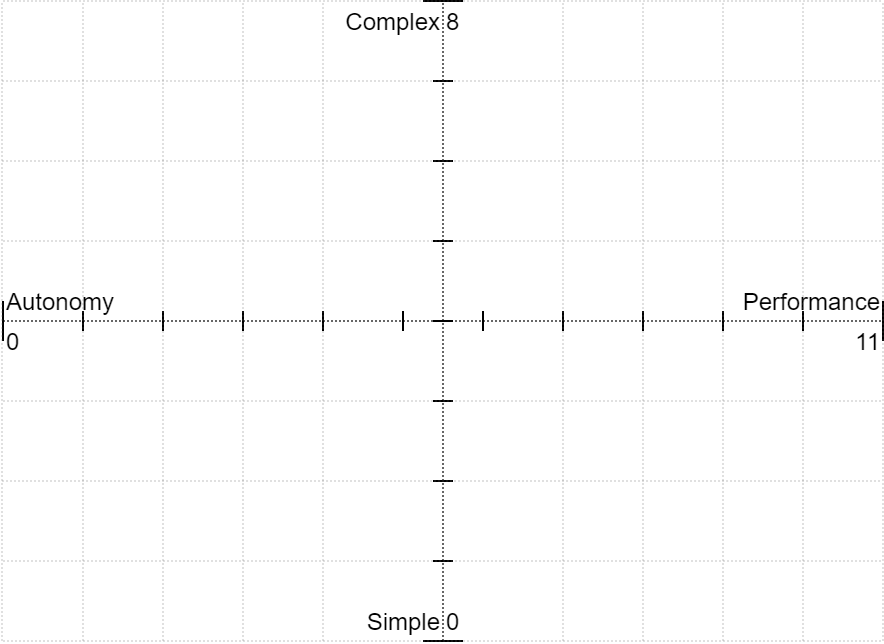
\includegraphics[scale=0.5]{quadrant_chart.png}
      \caption{Quadrant chart of the opposing questions, simplicity vs. complexity, and autonomy vs. performance}
      \label{img:quadrant_chart}
\end{figure}

The graph can be used to compare applications in one image.
It provides an overview of the driving affiliations for an application.
Both assessment Tables \ref{tbl:application_assessment} and \ref{tbl:shell_assessment} only reflect the amount of approaches taken into a certain direction, rather than actually outlining how strong an application invests into any of the directions.
Therefore, it is hard to determine the significance of this chart, but it is a first approach on providing an overview.





\subsection{Analysis conclusion}

The requirement analysis resulted in 23 requirements and many approaches.
To better outline which of the requirements are actually important, they are firstly grouped into categories.
These categories were then ordered by importance, see \ref{cha:requirement_categories}.
After that, the requirements within each categories were ordered by importance, see \ref{cha:requirements_overview}.
Finally, each requirement with their approaches are explained, which resulted in many cross-references and partially overlapping information.
Therefore, the section \ref{cha:requirements_conclusion} outlines important facts that became apparent while working on the requirement analysis.
The section \ref{cha:requirements_conclusion_assessment} is used in the next chapter to compare different applications against each other.




% Evaluation
%!TEX root = ../documentation.tex

\chapter{Evaluation}\label{cha:evaluation}

The previous chapter provides all the information needed to evaluate whether a generalized shell application is needed and how it would look like.
In the following the experts opinion on this question is presented, which concludes the experts input to this thesis.
Afterwards, one practical example for each scenario from \ref{cha:scenarios_types} is shown.
This will be used to evaluate if the most mentioned framework from the experts can fulfill all the needs outlined in the chapter \ref{cha:requirement}.





\section{Expert opinions}\label{cha:evaluation_experts}

The final question of the expert interviews was the thesis question, \ref{cha:appendix_expertinterview_questions}.
It is, whether a generalized shell application is needed or not.
All experts believe, that something is needed, but some are more precise of what is actually needed.
One framework was mentioned by \textciteRehm{}, \textciteMezzalira{}, \textciteJovanovic{} and \textciteSteyer{}, namely \textit{Single-SPA}.
This is the most known \ac{MF} framework.
They believe, that it is at least a step into the right direction in fulfilling the need of a generalized shell application.

\textit{Single-SPA} is a meta framework, which means it manages other frameworks (more information is provided in the section \ref{cha:evaluation_singlespa}).
\citeauthorMezzalira{} points out, that he believes the approach they have built for DAZN is slightly more flexible than \textit{Single-SPA}.
Still, if he had known of \textit{Single-SPA} 3 years ago, he would have used it.

Besides this one practical approach, \textciteHuber{} points out that \ac{MFA} is still new, which is why no clear answer is available yet.
This is confirmed by \textciteJovanovic{} and \textciteOlleck{}.
\citeauthorJovanovic{} believes that an example application that can be customized for other projects would be great.
Such an application can be used as a showcase for new customers and as base for new projects.
As a result, this lowers the barrier to getting started with the \ac{MFA}.
On the other hand, \citeauthorOlleck{} thinks that an example is not enough and instead standards are needed.
These standards would allow to mitigate problems which all projects will face at some point.
This could include for example, how to manage shared state or how to handle intercommunication.
However, he points out, that not everything can be standardized, because there are custom needs for each shell implementation as well.
Therefore, \citeauthorOlleck{} and also \citeauthorSteyer{} believe, that a shell framework is needed instead of a generalized shell application.

To sum up, the framework \textit{Single-SPA} was mentioned by almost all experts which also believe it could fulfill the need.
This will be evaluated in section \ref{cha:evaluation_singlespa}.
In general all experts agree on the idea that some form of generalized shell is needed.





\section{Application examples}\label{cha:evaluation_example}

Before evaluating \textit{Single-SPA}, it is important to outline what actual applications look like in terms of approaches.
This helps to set goals, which \textit{Single-SPA} needs to achieve in order to pass as general shell application.
The example applications are meant to cover a wide range of requirement combinations and still fit into the named scenarios from \ref{cha:scenarios_types}.
Hence, the facts named in section \ref{cha:scenarios_types} are used to determine which requirements are needed.
From these facts, only integration requirements can be extracted from them.
The structure of this section is, that the examples are explained, then some common facts are outlined and finally the assessment based on \ref{cha:requirements_conclusion_assessment} is conducted.



\paragraph{\nameref{cha:scenarios_enterprise} (EA)}\label{cha:evaluation_enterprise}

Before describing the enterprise application example, it helps to first outline what the differences are to other application types in regards to integration requirements.
An \nameref{cha:scenarios_enterprise} has no need for the \nameref{cha:requirement_detail_integration_crawler} requirement, because it is typically developed in-house and therefore no search engine needs to index the application.
Another needless requirement is \nameref{cha:requirement_detail_integration_abstraction}, because such an application is typically not used from a game console or smart TV.
The same applies for the \nameref{cha:requirement_detail_integration_extensible} requirement, because the application must be used by multiple companies so that extensions are created.
On the other hand, it is possible that a \ac{MF} is reused in multiple applications and therefore the \nameref{cha:requirement_detail_integration_interoperable} requirement could be needed.

After outlining the general integration requirement needs for an \nameref{cha:scenarios_enterprise}, an example enterprise application is shown to better emphasize the theoretical information.
This enterprise application example is mainly based on the application described by \textciteOlleck{}.
Its only difference is, that the \nameref{cha:requirement_detail_integration_lifecycle} requirement is not part of the application.
Based on the other experts inputs, there is no need for this requirement, if the target device is performant.
Also, this reduces the complexity for the shell and keeps the state of each \ac{MF}.

In case of page composition, both \nameref{cha:requirement_detail_integration_widget} and \nameref{cha:requirement_detail_integration_pagelayout} requirements are part of the example application.
The first is needed for cross cutting concern \ac{UI} elements and the latter only is needed for a tile-based arrangement.
Another requirement that can effect page composition, is part of this example, which is \nameref{cha:requirement_detail_integration_sharedlogic}.
It is needed to share the navigation bar and provide a shared toast feature.
Finally, in terms of the \nameref{cha:requirement_detail_state_exchange} requirement, a Redux store is selected, because of its superior bug fixing feature.

This concludes the \nameref{cha:scenarios_enterprise} example, because no more information would change the outcome of the quadrant chart described in \ref{cha:requirements_conclusion_assessment} and all integration requirements are considered.



\paragraph{\nameref{cha:scenarios_consumer} (CA)}\label{cha:evaluation_consumer}

Before describing the example, it helps to first outline what the differences are to other application types in regards to integration requirements.
While the \nameref{cha:requirement_detail_integration_crawler} requirement is not needed for a \nameref{cha:scenarios_enterprise}, it is certainly a relevant feature for a \nameref{cha:scenarios_consumer}.
However, its importance varies:
For example, an e-commerce shop needs the requirement, while a banking application could be fine without it.
Another requirement which is needed is \nameref{cha:requirement_detail_integration_abstraction}, as outlined by \textciteMezzalira{}.
In his example, the application DAZN needs to work in game console and smart TV browsers.
A probably rare requirement is \nameref{cha:requirement_detail_integration_extensible}.
For this \textciteSteyer{} provided the example, that gaming or gambling applications sometimes include third party applications via iFrames.
Hence, it is relevant for a \nameref{cha:scenarios_consumer}.
On the other hand, it is unlikely that a \ac{MF} is needed in multiple applications.
As a result, \nameref{cha:requirement_detail_integration_interoperable} is left out.

Similarly to the previous scenario, an example application is presented as well.
This example is mainly based on the application described by \textciteMezzalira{}.
The example application has two differences compared to the described application by \citeauthorMezzalira{}.
First, it includes the \nameref{cha:requirement_detail_integration_widget} requirement to allow for cross cutting \acp{UI} and second the \nameref{cha:requirement_detail_integration_sharedlogic} requirement is added to share the navigation panel.

The scenario application from \textciteMezzalira{} also uses the \nameref{cha:requirement_detail_integration_lifecycle} requirement to dereference unused \acp{MF}.
Moreover, because there is no need for multiple \acp{MF} per page, the \nameref{cha:requirement_detail_integration_pagelayout} requirement is not part of the example application.
Another aspect was already explained in the beginning, which is the \nameref{cha:requirement_detail_integration_abstraction} requirement.
This is part of the example, because it should work on consoles and smart TV browsers as well.
Finally, for the \nameref{cha:requirement_detail_state_exchange} requirement the shell is responsible to cache \ac{API} fetches to reduce duplicate requests.



\paragraph{\nameref{cha:scenarios_offshelf} (OA)}\label{cha:evaluation_offshelf}

Finally, there is the \nameref{cha:scenarios_offshelf}.
It is essentially a mix of \nameref{cha:scenarios_enterprise}s and \nameref{cha:scenarios_consumer}s, which was outlined in \ref{cha:scenarios_types}.
Also, only \textcite{Grijzen.2019} provided information about this application type, which does not allow to generalize it.
Therefore, the application he describes is used as the example application.

\textcite{Grijzen.2019} describes an application that monitors other applications.
The application needs a flexible layout, thus the \nameref{cha:requirement_detail_integration_pagelayout} requirement is needed.
But they do not need the \nameref{cha:requirement_detail_integration_widget} requirement.
Another requirement that is not needed is the \nameref{cha:requirement_detail_integration_abstraction}.

A priority for the application is performance, which is why code and data is shared as much as possible.
As a result, only one version of React is used and common dependencies are shared.
In the application a library is used to cache fetch data from an endpoint.
Hence, fetch data is cached, but the complexity is not within the shell.
Another aspect which accounts into sharing is the \nameref{cha:requirement_detail_integration_sharedlogic} requirement.
In case of the application \citeauthor{Grijzen.2019} describes that the navigation panel is part of the shell and is dynamically rendered.
Furthermore, a platform \ac{API} is shared over the shell with all \acp{MF} for common actions.
Finally, the \nameref{cha:requirement_detail_integration_lifecycle} requirement was not mentioned by him.
Because the other requirements heavily favor performance, it can be suspected, that it is part of the application.

% requirements:
% \xmark{} \nameref{cha:requirement_detail_integration_crawler}, because the app is not public (its a monitoring tool)
% \cmark{} \nameref{cha:requirement_detail_integration_interoperable}, was main goal
% \xmark{} \nameref{cha:requirement_detail_integration_abstraction}, no need to run on consoles or smart TVs
% \cmark{} \nameref{cha:requirement_detail_integration_extensible}



\paragraph{Common facts}

\begin{table}
    \begin{tabular}{|l|cc|cc|}
        \multirow{2}{*}{\textbf{Requirement}}                                  &
        \multicolumn{2}{c|}{\textbf{\hyperref[cha:evaluation_enterprise]{EA}}} &
        \multicolumn{2}{c|}{\textbf{\hyperref[cha:evaluation_consumer]{CA}}}
        \\
                                                                               &
        \multicolumn{1}{c|}{mandatory}                                         &
        optional                                                               &
        \multicolumn{1}{c|}{mandatory}                                         &
        optional
        \\ \hline
        \nameref{cha:requirement_detail_integration_loading}                   & \cmark{} &          & \cmark{} &          \\
        \nameref{cha:requirement_detail_integration_lifecycle}                 &          & \cmark{} & \cmark{} &          \\
        \nameref{cha:requirement_detail_integration_routing}                   & \cmark{} &          & \cmark{} &          \\
        \nameref{cha:requirement_detail_integration_configuration}             & \cmark{} &          & \cmark{} &          \\
        \nameref{cha:requirement_detail_integration_integration}               & \cmark{} &          & \cmark{} &          \\
        \nameref{cha:requirement_detail_integration_crawler}                   &          &          &          & \cmark{} \\
        \nameref{cha:requirement_detail_integration_sharedlogic}               &          & \cmark{} &          & \cmark{} \\
        \nameref{cha:requirement_detail_integration_widget}                    &          & \cmark{} &          & \cmark{} \\
        \nameref{cha:requirement_detail_integration_pagelayout}                &          & \cmark{} &          & \cmark{} \\
        \nameref{cha:requirement_detail_integration_interoperable}             &          & \cmark{} &          &          \\
        \nameref{cha:requirement_detail_integration_abstraction}               &          &          &          & \cmark{} \\
        \nameref{cha:requirement_detail_integration_extensible}                &          &          &          & \cmark{}
    \end{tabular}
    \centering
    \caption{Overview of integration requirement distribution between \nameref{cha:scenarios_enterprise}s and \nameref{cha:scenarios_consumer}s}
    \label{tbl:evaluation_requirement_distribution}
\end{table}

While defining the example applications based on the experts inputs, there are some facts that became apparent, which need to be outlined.
The first fact was hinted in the examples, which is that there are some similarities between the example application requirements.
Table \ref{tbl:evaluation_requirement_distribution} shows which integration requirements are needed or optional for the \nameref{cha:scenarios_enterprise} and \nameref{cha:scenarios_consumer}, based on the examples.
Also, because the \nameref{cha:scenarios_offshelf} is a mix of the other two, it is not included in the Table.
Abbreviations for the application type names are applied in the Table, which are \nameref{cha:scenarios_enterprise} is \textit{EA}, \nameref{cha:scenarios_consumer} is \textit{CA} and \nameref{cha:scenarios_offshelf} is \textit{OA}.

The Table \ref{tbl:evaluation_requirement_distribution} visualizes two findings.
The first is that the requirements \nameref{cha:requirement_detail_integration_loading}, \nameref{cha:requirement_detail_integration_routing}, \nameref{cha:requirement_detail_integration_configuration} and \nameref{cha:requirement_detail_integration_integration} are always needed.
This is in line with the experts statements for the interview question five, which determines critical requirements for a shell application.
An overview of which requirement was mentioned for what question, is shown in Table \ref{tbl:adx_requirements_references}.
The only outlier in regards to the interview question five answers, is the \nameref{cha:requirement_detail_integration_lifecycle} requirement.
This requirement is considered critical by \textciteRehm{}, but not universally needed.
It is rather only needed for performance oriented applications.

The second finding is, that \nameref{cha:requirement_detail_integration_widget}, \nameref{cha:requirement_detail_integration_pagelayout} and \nameref{cha:requirement_detail_integration_sharedlogic} are optional in both cases.
The first two requirements mainly address page composition (see \ref{cha:theroy_extensions_composition}) whereas the last is about sharing \ac{UI} or common business functions.
All three requirements are important for the general structure of the application, but they are optional.



\paragraph{Assessment}

\begin{table}
    \setlength{\tabcolsep}{5pt} % Default value: 6pt
    \begin{tabular}{|c|l|cc|cc|cc|}
        \multicolumn{2}{|c|}{\textbf{Requirements}}                                    &
        \multicolumn{2}{c|}{\textbf{\hyperref[cha:evaluation_enterprise]{EA}}}         &
        \multicolumn{2}{c|}{\textbf{\hyperref[cha:evaluation_consumer]{CA}}}           &
        \multicolumn{2}{c|}{\textbf{\hyperref[cha:evaluation_offshelf]{OA}}}
        \\
        Shell                                                                          &
        \multicolumn{1}{c|}{Application (App)}                                         &
        \multicolumn{1}{c|}{Shell}                                                     &
        App                                                                            &
        \multicolumn{1}{c|}{Shell}                                                     &
        App                                                                            &
        \multicolumn{1}{c|}{Shell}                                                     &
        App
        \\ \hline
        \multicolumn{2}{|c|}{\nameref{cha:requirement_detail_integration_pagelayout}}  &
        1                                                                              & 0          & 0          & 1          & 1          & 0                       \\
        \multicolumn{2}{|c|}{\nameref{cha:requirement_detail_integration_widget}}      &
        1                                                                              & 1          & 1          & 1          & 0          & 0                       \\
        \multicolumn{2}{|c|}{\nameref{cha:requirement_detail_integration_abstraction}} &
        0                                                                              & 0          & 1          & 1          & 0          & 0                       \\
        \multicolumn{2}{|c|}{\nameref{cha:requirement_detail_state_exchange}}          &
        0                                                                              & 2          & 2          & 1          & 1          & 0                       \\
        \multicolumn{2}{|c|}{\nameref{cha:requirement_detail_integration_sharedlogic}} &
        2                                                                              & 2          & 1          & 1          & 2          & 2                       \\
        \multicolumn{1}{|l|}{\nameref{cha:requirement_detail_integration_lifecycle}}   &
        \makecell[l]{\hyperref[cha:requirement_detail_performance]{Performance}                                                                                      \\(shared dependencies)} &
        0                                                                              & 0          & 1          & 1          & 1          & 2                       \\
        \multicolumn{1}{|l|}{- }                                                       &
        \makecell[l]{\hyperref[cha:requirement_detail_performance]{Performance}                                                                                      \\(shared core)} &
        -                                                                              & 0          & -          & 2          & -          & 2                       \\ \hline
        \multicolumn{2}{|r|}{\textbf{Sum}}                                             & \textbf{4} & \textbf{5} & \textbf{6} & \textbf{8} & \textbf{5} & \textbf{6}
    \end{tabular}
    \centering
    \caption{Example application evaluation result scores}
    \label{tbl:eval_app_scores}
\end{table}

\begin{figure}
    \centering
    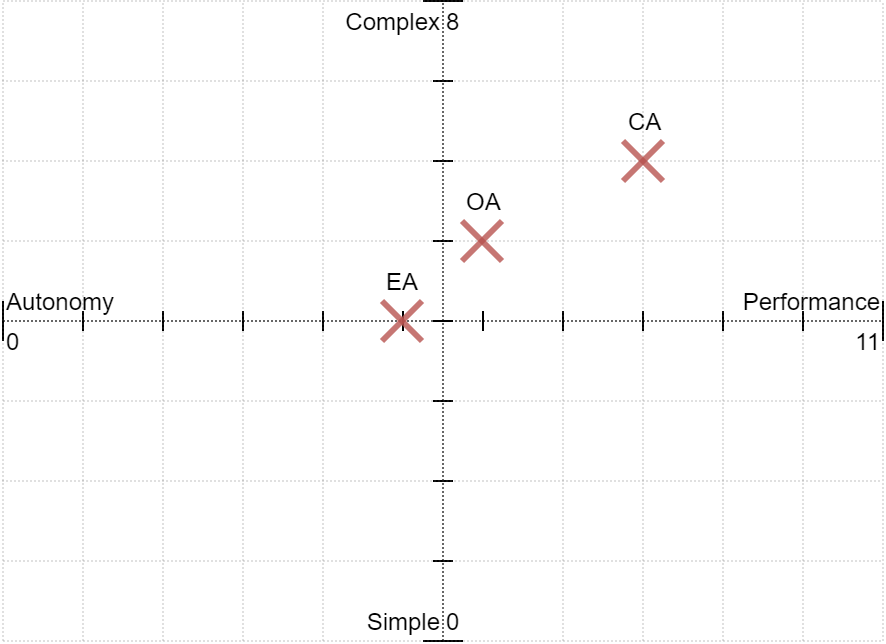
\includegraphics[scale=0.5]{quadrant_chart_filled.png}
    \caption{Quadrant chart from \ref{img:quadrant_chart} filled with evaluation results of the example applications}
    \label{img:quadrant_chart_filled}
\end{figure}


The named example applications are assessed, based on the score metric of section \ref{cha:requirements_conclusion_assessment}.
The evaluation result is shown in Table \ref{tbl:evaluation_requirement_distribution} and visualized in Figure \ref{img:quadrant_chart_filled}.
These examples satisfy the conceptual need for example applications, mentioned by \textciteJovanovic{}, which only leaves the need for an actual implementation.
An interesting fact shown in the Figure \ref{img:quadrant_chart_filled} is, that there seems to be a connection between the shell complexity and application performance.




\section{Existing solution Single-SPA}\label{cha:evaluation_singlespa}

The final part of this thesis is to evaluate, whether or not an existing framework fulfills all needs.
The framework in question is \textit{Single-SPA}, because it was mentioned by four of the six experts, which are namely \textciteRehm{}, \textciteMezzalira{}, \textciteJovanovic{} and \textciteSteyer{}.
There are two main things, which are evaluated.
The first is to check which requirements can be satisfied and secondly if \textit{Single-SPA} could be used to realize the example applications.

Based on the \textit{Single-SPA} documentation \cite{singlespa.2020}, all requirements and examples are feasible.
But there are some important aspects, which need to be outlined.
First and foremost, it fully depends on SystemJS.
SystemJS is a polyfill for \ac{ES}6 features that are not yet supported in browsers\footnotemark.
\footnotetext{\url{https://github.com/systemjs/systemjs} (Visited on 08/13/2020)}
It allows using a feature called \textit{Import Maps}.
Usually an import statement needs a \ac{URL} in the browser, but this browser specification allows to define an alias instead.
As a result, all \ac{JS} import statements can use the alias and the \ac{URL} is only set once in the \textit{Import Map}\footnotemark.
\footnotetext{\url{https://exploringjs.com/es6/ch_modules.html} (Visited on 08/13/2020)}

SystemJS supports this feature by providing a module loader implementation, which must be used instead of the native import statement.
Hence, all dependencies need to be transpiled into the SystemJS format in order to be used at all.
The transpilation can be handled by Webpack for instance.
While it adds some overhead, it allows to directly import code instead of providing it over a global variable.

Another aspect that is needed to implement many requirements is the shared Utility feature of \textit{Single-SPA} \cite{singlespa.2020}.
The \textit{Single-SPA} shell only provides features for the requirements \nameref{cha:requirement_detail_integration_loading}, \nameref{cha:requirement_detail_integration_lifecycle}, \nameref{cha:requirement_detail_integration_routing}, \nameref{cha:requirement_detail_integration} and \nameref{cha:requirement_detail_integration_widget}.
Other features are not provided out of the box, but can be realized with sharing Utility functions.
This addresses the \nameref{cha:requirement_detail_integration_abstraction}, \nameref{cha:requirement_detail_integration_sharedlogic}, \nameref{cha:requirement_detail_state_exchange},  \nameref{cha:requirement_detail_state_intercommunication} and \nameref{cha:requirement_detail_state_security} requirements, as well as styles from the \hyperref[cha:requirement_detail_style]{Consistent style} requirement.
This leaves the complexity out of the shell, while each project needs to implement it on its own.

The \nameref{cha:requirement_detail_integration_configuration} requirement is restricted in its flexibility.
Adding \acp{MF} is only possible via \ac{JS} code.
As a result, the \nameref{cha:requirement_detail_integration_extensible} requirement is possible, but it must be added via \ac{JS} code.
The final aspect for the requirements is, that the \textit{Single-SPA} feature which allows for the \nameref{cha:requirement_detail_integration_pagelayout} requirement is currently in a beta phase.
The feature is called Layout Engine \cite{singlespa.2020}.

While evaluating if the examples are theoretically feasible, there are three additional aspects that came up.
First, a Redux Store for the \hyperref[cha:evaluation_enterprise]{\nameref{cha:scenarios_enterprise}} example can be used in combination with \textit{Single-SPA}, although the team of \textit{Single-SPA} does not recommended using a global Redux store in general.
Next up is the caching approach for the \hyperref[cha:evaluation_consumer]{\nameref{cha:scenarios_consumer}} example.
This can be realized via a shared Utility function.
And finally, any shared dependencies or shared framework cores are distributed via SystemJS.


Ultimately \textit{Single-SPA} can achieve everything needed for a \ac{MF} application.
There are also two additional statements from the experts to it.
\textciteSteyer{} points out, that a \textit{Single-SPA} \ac{MF} can not be loaded in standalone mode.
This is a feature he demands, that \textit{Single-SPA} currently lacks.
The second statement is from \textciteMezzalira{} who states that \textit{Single-SPA} has a \enquote{opinionated} way of implementing \acp{MF}.
He did not further specify what he exactly means, but this may be that loading and importing is handled by SystemJS.



% Architecture
%!TEX root = ../documentation.tex

% \chapter{Architecture}\label{cha:architecture}
% % titel vorschlag: architektur empfehlung
% % man könnte theoretisch auch 

% \textcite[p.~13]{Fielding.2000} said that, properties are induced by the set of constraints within an architecture.
% % see: https://youtu.be/WlsetrZgSMQ?t=1123
% Which means that architectural design choices for a project will yield certain characteristics for the solution.
% In chapter \ref{cha:requirement} possible requirements are discussed and these are the constraints for the architecture.
% Thus, the shell architecture needs to be able to support these constraints.
% It is important to mention, that there are also custom business constraints which can effect the shell.
% This results in the need for a flexible architecture.

% There two possible architectural techniques to achieve the needed flexibility for a shell application.
% The first one is a base implementation which is modular and allows for plugins and the second is creating a framework which solve the common problems.






% Fazit
%!TEX root = ../documentation.tex

\chapter{Conclusion}\label{cha:conclusion}

Even though the \acf{MFA} is gaining traction nowadays, there are many developers and architects who are still uncomfortable with it.
One aspect that contributes to this, is that there is a lack of knowledge and experience in this field.
In addition, newcomers and experts would also prefer a general implementation for reusing parts in a \ac{MF} application.
This need is satisfied to a certain extent in this thesis, but only for the approach \textit{Client-Side} integration via shell application.


To address the lack of knowledge, the chapter \ref{cha:Theory} introduces the \ac{MFA} fundamentals.
This is then followed up by outlining when to use the architecture, in chapter \ref{cha:scenarios}.
After describing what it is and when to use it, the next step is to show different facades of it.
This is done in chapter \ref{cha:requirement}, by detailing different requirements and their approaches, as well as highlighting overlapping facts about the approaches in the end.
The final chapter \ref{cha:evaluation} uses the collected information to address thesis questions.

The first question is if there is a general need for a generalized shell application.
This could be confirmed by all interviewed experts, see \ref{cha:evaluation_experts}.
However, this leaves the question open how such a generalized shell application looks like.
All features which should be supported are outlined in the requirement analysis.
Also, to further provide insights about the structure of such an application, the section \ref{cha:evaluation_example} provides example applications that a shell application must be able to handle.
As a result, a fresh view about the \ac{MFA} implementation is provided.
It is compared to the approach which is provided by \textit{Single-SPA}.
This shows, that \textit{Single-SPA} can fulfill all needs outlined by the requirements analysis. 
However, many requirements are realized via the shared utility feature, which is explained in \ref{cha:evaluation_singlespa}.

In addition to the introductory question, further results have been identified in the course of this work.
First and foremost, as it turns out, the requirement analysis section from \ref{cha:requirement_detail_integration} till \ref{cha:requirement_detail_developer} are a good approach reference guide for most of the requirements.
Secondly, the section \ref{cha:requirements_conclusion} outlines approaches that are used in multiple requirements and most interestingly a metric to assess \ac{MF} applications and their shell implementations.

Regardless of the results of this work, there are still points that need further investigation.
First of all, the experts opinions are mostly not challenged and considered as the truth.
This means that further practical work would be required to check if the expert opinions can be applied in general.
Although there is an overview of which expert mentioned which requirement, which allows to sort the requirements based on the amount of mentions, see \ref{tbl:adx_requirements_references}.
This simplifies the continuation of this work in terms of checking the requirement importance.
Furthermore, in the beginning a differentiation between the two types of experts who have already used \acp{MF} for a while and experts which are currently learning and implementing the architecture, is drawn.
This differentiation was not taken into consideration while scoring any requirements.
The reason for this is that the number of experts per type is not enough to be significantly comparable.
It could have provided insights into what are challenges at the start and and later on.
However, this is not further investigated in this work, which leaves it open for future work.

After considering several requirements and expert opinions on the topic of \acp{MF}, the question remains open as to how to proceed.
An important feature that is missing for developer experience is a client-side \ac{CDC} testing approach.
This is also addressed in the \nameref{cha:requirement_detail_developer_testing} requirement.
A possible concept could be to define a standardized \ac{MF} intercommunication and using this standard environment to build a tool that enables testing this environment.
A practical solution could be to use a global Redux store that tracks the internal actions of a \ac{MF} and a mock \ac{MF} as communication partner.
The mock \ac{MF} either consumes messages and either records these or publishes recorded messages.
These recordings could be in line with the Redux stores recorded actions to get the timing right.
This approach would limit the freedom of the developer in terms of choosing a lighter approach than a Redux store.

In addition, a further question remains open in regards to the section \ref{cha:requirements_conclusion_assessment}. It could not be clarified in more detail whether the scenario implies a certain score in the assessment.
One could make the following assumption, that an \nameref{cha:scenarios_enterprise} would typically require a simple shell as well as autonomous teams, while \nameref{cha:scenarios_consumer} tends to a more complex shell which could improve the performance of the application.
Consequent evaluations whether there is such a connection may be interesting, but will require further research.
Such an evaluation would imply the need to assess the scoring of the assessment as well.
This is due to the fact that currently only the amount of approaches taken into a certain direction are considered, rather than the actual property.


To conclude, it can be summarized that some experts believe that a framework would be a better solution than a generalized application for the shell implementation.
It would still be necessary to evaluate by means of a practical example whether a framework would really be better than an own customized implementation for the shell.
In this regard, the framework \textit{Single-SPA} can be used as a reference, since it already covers many requirements.



% Inhalt
%\foreach \i in {01,02,03,04,05,06,07,08,09,...,99} {%
%	\edef\FileName{content/\i kapitel}%
%		\IfFileExists{\FileName}{%
%			\input{\FileName}
%		}
%		{%
%			%file does not exist
%		}
%}

\clearpage

\pagenumbering{roman}
\setcounter{page}{\number\value{savepage}}

% Literaturverzeichnis
\cleardoublepage
\printbibheading
\printbibliography[nottype=online,heading=subbibliography,title={Publications}]
\printbibliography[type=online,notkeyword=Gesetz,notkeyword=Standard,heading=subbibliography,title={Online References}]
\printbibliography[type=online,keyword=Gesetz,heading=subbibliography,title={Rechtsquellenverzeichnis}]
\printbibliography[type=online,keyword=Standard,heading=subbibliography,title={Standards \& Normen}]

%	\renewcommand\bibname{Literaturverzeichnis}
%	\printbibliography

%	\newpage\null\thispagestyle{plain}\newpage

% Glossar
\printglossary[style=altlist,title=\langglossar]

% sonstiger Anhang
\clearpage
\appendix
% !TeX root = ../documentation.tex

\addchap{\langanhang}

\chapter{Expert interview procedure}\label{cha:appendix_expertinterview}

This was used as guideline for the expert interviews.
There is also a \ac{GDPR} clause, but it is not included.

\section{General procedure of interviews}

First, I will introduce myself, my bachelor thesis and explain the interview procedure. After that, I would start the recording, read the \ac{GDPR} clause loudly and ask you if it is ok for you. Then you should shortly introduce yourself and outline your work experience. Next, I start asking you the interview questions.

\textbf{More information about the questions}

Nearly all questions ask about requirements. This term includes requirements from the party’s customer, consumer (end user) and developer. There are also scenarios mentioned. The general intention is to cluster requirements around scenarios so that readers can better grasp when a requirement is needed. This also allows finding the most needed requirements.

\textbf{Requirements categories of interest}

There are all sorts of requirements for a micro frontend application. So, to ensure that the same categories are interviewed and to shift the focus to the important requirements, the following list was created. The list shows the importance descending, as well as examples for shared state and developer experience.

\begin{enumerate}
    \item Browser routing and integration approach
    \item Performance
    \item Shared state and micro frontend inter-communication techniques
          \begin{itemize}
              \item Internationalization
              \item Authentication
              \item Etc.
          \end{itemize}
    \item Styling handling
    \item Developer experience
          \begin{itemize}
              \item Tools
              \item Debugging
              \item Testing
          \end{itemize}
\end{enumerate}

\section{Interview Questions}\label{cha:appendix_expertinterview_questions}

\begin{enumerate}
    \item Have you worked with a micro frontend shell application?
          \begin{itemize}
              \item Yes: Could you name general facts? (used frameworks, team size, general structure)
              \item No: why not?
          \end{itemize}
    \item What are suitable scenarios for the micro frontend architecture in general?
    \item What do you think about my requirement categories? Am I missing anything? Would you change the order of importance?
    \item What are requirements for the named shell application scenario which you had from a customer?
          \begin{itemize}
              \item If possible, also add which approach was used and or considered
              \item If you are not allowed to share this information, answer the question with what you think are the needed requirements.
          \end{itemize}
    \item Can you name any requirements which are needed for all shell application scenarios?
          \begin{itemize}
              \item If possible, also add which approach was used.
          \end{itemize}
    \item What are the most difficult requirements to achieve and why?
    \item Do you think that there is a need for a generalized shell application?
\end{enumerate}

\chapter{Requirement evaluation}\label{cha:appendix_requirements_overview}

The Table \ref{tbl:adx_requirements_scores} contains all requirements and there score.
The base for this calculation is shown in Table \ref{tbl:adx_requirements_references}, which contains all references were these requirements were mentioned, considered difficult or considered critical.
The process is explained in \ref{cha:requirement}.
In the Table \ref{tbl:adx_requirements_scores} a \ac{ID} is introduced, which is used in Table \ref{tbl:adx_requirements_references}.

The following list shows all references used in the Table \ref{tbl:adx_requirements_references} and there last names.
\begin{itemize}
    \item \textcite{Dornenburg.2019}
    \item \textcite{Grijzen.2019}
    \item \textcite{Jackson.2019}
    \item \textcite{Laug.2018}
    \item \textcite{Leitner.2020}
    \item \textciteOlleck{}
    \item \textciteJovanovic{}
    \item \textciteMezzalira{}
    \item \textciteSteyer{}
    \item \textciteHuber{}
    \item \textciteRehm{}
\end{itemize}



\begin{table}[]
    \begin{tabular}{|l|l|l|l|}
        \hline
        \textbf{\ac{ID}}  &
        \textbf{Score}    &
        \textbf{Category} &
        \textbf{Requirement}
        \\ \hline
        1                 & 14 & Integration & Loading                \\ \hline
        2                 & 10 & Integration & Lifecycle management   \\ \hline
        3                 & 9  & Integration & Routing                \\ \hline
        4                 & 8  & Integration & Configuration          \\ \hline
        5                 & 7  & Integration & Integration            \\ \hline
        6                 & 6  & Integration & Shared logic           \\ \hline
        7                 & 4  & Integration & Widgets                \\ \hline
        8                 & 4  & Integration & Page layout            \\ \hline
        9                 & 2  & Integration & Indexable via crawler  \\ \hline
        10                & 2  & Integration & \ac{MF} interoperable  \\ \hline
        11                & 1  & Integration & Abstraction layer      \\ \hline
        12                & 1  & Integration & Third party extensible \\ \hline
        13                & 11 & Performance & Performance            \\ \hline
        14                & 16 & State       & State exchange         \\ \hline
        15                & 10 & State       & Intercommunication     \\ \hline
        16                & 5  & State       & Security               \\ \hline
        17                & 2  & State       & Internationalization   \\ \hline
        18                & 15 & Style       & Consistent style       \\ \hline
        19                & 13 & Developer   & Autonomy               \\ \hline
        4                 & 8  & Developer   & Configuration          \\ \hline
        20                & 8  & Developer   & Experience             \\ \hline
        21                & 5  & Developer   & Tools                  \\ \hline
        22                & 3  & Developer   & Debugging              \\ \hline
        23                & 3  & Developer   & Testing                \\ \hline
    \end{tabular}
    \caption{Overview of all requirements with scores}
    \label{tbl:adx_requirements_scores}
\end{table}




\begin{table}[]
    \begin{tabular}{|l|l|l|l|}
        \hline
        \textbf{\ac{ID}}   &
        \textbf{Mentioned} &
        \textbf{Difficult} &
        \textbf{Critical}
        \\ \hline
        1                  & \cite{Dornenburg.2019}, \cite{Grijzen.2019}, \cite{Vogel.2020.Huber}, \cite{Jackson.2019}, \cite{Leitner.2020}, \cite{Laug.2018}, \cite{Vogel.2020.Steyer}     &                                                                                                              & \cite{Vogel.2020.Jovanovic}, \cite{Vogel.2020.Rehm}                           \\ \hline
        2                  & \cite{Dornenburg.2019}, \cite{Grijzen.2019}, \cite{Leitner.2020}, \cite{Vogel.2020.Mezzalira}, \cite{Vogel.2020.Olleck}                                        &                                                                                                              & \cite{Vogel.2020.Rehm}                                                        \\ \hline
        3                  & \cite{Dornenburg.2019}, \cite{Grijzen.2019}, \cite{Vogel.2020.Huber}, \cite{Laug.2018}, \cite{Vogel.2020.Rehm}, \cite{Vogel.2020.Steyer}                       & \cite{Vogel.2020.Mezzalira}                                                                                  &                                                                               \\ \hline
        4                  & \cite{Grijzen.2019}, \cite{Vogel.2020.Rehm}                                                                                                                    &                                                                                                              & \cite{Vogel.2020.Jovanovic}                                                   \\ \hline
        5                  & \cite{Laug.2018}, \cite{Vogel.2020.Rehm}, \cite{Vogel.2020.Steyer}                                                                                             &                                                                                                              &                                                                               \\ \hline
        6                  & \cite{Dornenburg.2019}, \cite{Jackson.2019}, \cite{Laug.2018}                                                                                                  &                                                                                                              &                                                                               \\ \hline
        7                  & \cite{Dornenburg.2019}, \cite{Laug.2018}, \cite{Vogel.2020.Rehm}                                                                                               & \cite{Vogel.2020.Mezzalira}, \cite{Vogel.2020.Steyer}, \cite{Vogel.2020.Olleck}, \cite{Vogel.2020.Jovanovic} & \cite{Vogel.2020.Huber}                                                       \\ \hline
        8                  & \cite{Vogel.2020.Olleck}, \cite{Vogel.2020.Rehm}, \cite{Vogel.2020.Steyer}                                                                                     & \cite{Vogel.2020.Mezzalira}, \cite{Vogel.2020.Jovanovic}                                                     & \cite{Vogel.2020.Huber}                                                       \\ \hline
        9                  & \cite{Grijzen.2019}, \cite{Vogel.2020.Huber}, \cite{Vogel.2020.Mezzalira}, \cite{Vogel.2020.Rehm}                                                              & \cite{Vogel.2020.Jovanovic}                                                                                  & \cite{Vogel.2020.Steyer}                                                      \\ \hline
        10                 & \cite{Dornenburg.2019}, \cite{Grijzen.2019}, \cite{Leitner.2020}, \cite{Vogel.2020.Mezzalira}, \cite{Vogel.2020.Olleck}                                        &                                                                                                              & \cite{Vogel.2020.Rehm}                                                        \\ \hline
        11                 & \cite{Vogel.2020.Huber}, \cite{Laug.2018}, \cite{Vogel.2020.Mezzalira}, \cite{Vogel.2020.Rehm}, \cite{Vogel.2020.Steyer}                                       & \cite{Vogel.2020.Olleck}                                                                                     &                                                                               \\ \hline
        12                 & \cite{Dornenburg.2019}, \cite{Grijzen.2019}, \cite{Laug.2018}, \cite{Vogel.2020.Olleck}, \cite{Vogel.2020.Rehm}, \cite{Vogel.2020.Steyer}                      &                                                                                                              &                                                                               \\ \hline
        13                 & \cite{Dornenburg.2019}, \cite{Vogel.2020.Huber}                                                                                                                & \cite{Vogel.2020.Rehm}                                                                                       &                                                                               \\ \hline
        14                 & \cite{Grijzen.2019}, \cite{Laug.2018}, \cite{Vogel.2020.Mezzalira}, \cite{Vogel.2020.Olleck}                                                                   &                                                                                                              &                                                                               \\ \hline
        15                 & \cite{Dornenburg.2019}, \cite{Vogel.2020.Mezzalira}                                                                                                            &                                                                                                              &                                                                               \\ \hline
        16                 & \cite{Grijzen.2019}, \cite{Vogel.2020.Rehm}                                                                                                                    &                                                                                                              &                                                                               \\ \hline
        17                 & \cite{Vogel.2020.Mezzalira}                                                                                                                                    &                                                                                                              &                                                                               \\ \hline
        18                 & \cite{Grijzen.2019}                                                                                                                                            &                                                                                                              &                                                                               \\ \hline
        19                 & \cite{Dornenburg.2019}, \cite{Grijzen.2019}, \cite{Leitner.2020}                                                                                               & \cite{Vogel.2020.Olleck}                                                                                     & \cite{Vogel.2020.Steyer}, \cite{Vogel.2020.Rehm}                              \\ \hline
        4                  & \cite{Dornenburg.2019}, \cite{Grijzen.2019}, \cite{Jackson.2019}, \cite{Leitner.2020}, \cite{Laug.2018}                                                        & \cite{Vogel.2020.Olleck}                                                                                     & \cite{Vogel.2020.Jovanovic}, \cite{Vogel.2020.Steyer}, \cite{Vogel.2020.Rehm} \\ \hline
        20                 & \cite{Dornenburg.2019}, \cite{Grijzen.2019}, \cite{Jackson.2019}, \cite{Vogel.2020.Jovanovic}, \cite{Leitner.2020}, \cite{Laug.2018}, \cite{Vogel.2020.Steyer} &                                                                                                              & \cite{Vogel.2020.Olleck}                                                      \\ \hline
        21                 & \cite{Vogel.2020.Jovanovic}, \cite{Laug.2018}                                                                                                                  &                                                                                                              & \cite{Vogel.2020.Steyer}                                                      \\ \hline
        22                 & \cite{Vogel.2020.Mezzalira}, \cite{Vogel.2020.Steyer}                                                                                                          &                                                                                                              &                                                                               \\ \hline
        23                 & \cite{Dornenburg.2019}, \cite{Grijzen.2019}, \cite{Vogel.2020.Huber}, \cite{Jackson.2019}, \cite{Vogel.2020.Jovanovic}, \cite{Leitner.2020}, \cite{Laug.2018}  & \cite{Vogel.2020.Olleck}                                                                                     & \cite{Vogel.2020.Steyer}, \cite{Vogel.2020.Rehm}                              \\ \hline
    \end{tabular}
    \caption{Overview of all requirements and their respective references}
    \label{tbl:adx_requirements_references}
\end{table}





\chapter{Expert interview paraphrases}

Each interview starts with an introduction of the author and the bachelor thesis.
After that the interview guideline (\ref{cha:appendix_expertinterview}) is presented.
The following interview paraphrases represent the conversations after the interview guideline presentation.
The paraphrases does also not include the adoption.

% !TeX root = ../../documentation.tex

\section{Interview with Luca Mezzalira}

This paraphrase of the expert interview with Luca Mezzalira.
If any information of this is used in the thesis, its marked with \cite{Vogel.2020.Mezzalira}.
\textbf{V} is the abbreviation for \textit{Nico Vogel} and \textbf{M} for \textit{Luca Mezzalira}.

\setspeaker{LucaMezzalira}[M]

\begin{description}
    \NicoVogel The first question is, have you worked with micro frontend shell applications? I know that you have, thus, could you name general facts like the framework, the team size, general structure, and stuff like that.

    \LucaMezzalira So, we started to work with a shell application roughly 3 years ago. At that time, we were not aware of any other framework. Therefore, we created a way to handle that internally, which we called bootstrap. This has nothing to do with the well-known framework for creating responsive web applications. Instead, it is an application that is always available for the entire session of the user. It takes care of general tasks, like “loading micro frontends,” “routing between the micro frontends”, and exposing an API. The micro frontends require the API to manage their life cycle.
    The team size grew from 10 to 400 in 2 years’ time. These teams are distributed between 4 different locations in Europe.
    Micro frontends were introduced to bring the same benefits from the microservice architecture to the frontend. So, each team owns a specific part of the business domain. Therefore, they can independently make decisions needed for their domain.
    Another aspect that was important for the switch to micro frontends is that it is easier to incrementally upgrade the application. Furthermore, micro frontends allowed for a seamless transition from the old application to the new one.

    \NicoVogel The second question, what are suitable scenarios for micro frontend architectures in general. Like, one you already mentioned kind of. Can you mention any more?

    \LucaMezzalira I believe that micro frontends are a good architectural style when the organization is big or must scale the project. So, many developers work on the same project. To be more specific, if 50+ developers or distributed teams work on a frontend, micro frontend architecture should be considered. This architecture style is currently embraced by many organizations because of their infrastructure and communication channels.

    \NicoVogel What do you think about my requirements categories? Am I missing anything? Would you change the importance?

    \LucaMezzalira No category is missing. I would put as number 2 shared state, number 3 developer experience, number 4 performance, and number 5 style handling. If you do not invest in developer experience, there is no way that you are going to have a slick and smooth transition to micro frontends. Because using a micro-architecture adds a lot of complexity to a project. Performance is also important, but not especially different from a regular Single Page Application (SPA), for example. If you invest too much in performance, then you risk fading out some benefits of micro frontends, for example, the decoupling of teams or independent deployment. It is possible that a micro frontend architecture application might result in worse performance than a server-side rendering or pure SPA application.
    Next up is styling. Consistent styling can be achieved in different ways. One way is to use a Design System. It provides design tokens and simple components that should be used by each micro frontend. A Design System can also include a component library that consists of dumb components and elements, like buttons, labels, and so on. The micro frontend teams can use the component library to create more complex components.
    All these aspects are important, but you need to maintain a balance between the aspects. This essential in a distributed system like micro frontends.


    \NicoVogel What are requirements for the named shell application scenarios which you had for a customer? Maybe you could start with DAZN.

    \LucaMezzalira The application shell should be able to load micro frontend, route between micro frontends, expose certain configuration, handle live cycle methods, and if needed, it should also be an abstraction layer. The last feature is needed if the application is used across different devices with different browser APIs. Therefore, abstracting the domain-specific API from the platform. This allows for reusable micro frontends.

    \NicoVogel Can you also name a few approaches you took? You already mentioned that the shell is used as an abstraction layer. Can you name other requirements and their approaches, for example, routing?


    \LucaMezzalira DAZN has a unique approach on loading a micro frontend. For each micro frontend, there is one HTML file that is the entry point. This file contains all HTML import tags, which are required by the micro frontend. Using this approach appears to be faster than loading everything out of JavaScript, which has some overhead compared. The overhead consists of the framework and other business logic, which must run first before the actual loading is executed. On the other hand, the HTML approach is slim, and all that is needed is a function that adds the tags from the HTML file into the DOM. This approach is also quite flexible, and each domain can decide what to include in the entry point and whatnot. In terms of orchestration, the DAZN can support canary-releases and country-specific versions per micro frontend. This is archived by keeping the shell unaware of when and from where to load a micro frontend. Therefore, allowing for high granularity and flexibility. To enable this, releasing and shaping the traffic are two independent functions in the infrastructure of DAZN.

    \NicoVogel Can you name another scenario and requirements for that?

    \LucaMezzalira So, a different scenario to DAZN is that there are multiple micro frontends on the same page. On approach is that the shell knows every single view and how it looks like, which NewRelic did. They use a template approach that is handled by the shell. A template has placeholders, and the shell is responsible for filling them. I think the shell application knows a bit too much for my taste. In my opinion, the shell should be a transparent layer, which is very light and without any implications on how the micro frontends look or how they communicate with each other. The shell application should be completely decoupled from the micro frontends and only have some light touches of exposed functionality for the micro frontends. A micro frontend must be independently deployable. Otherwise, you are building a distributed monolith.

    \NicoVogel Did they use Single-SPA because it sounded like it.

    \LucaMezzalira Single-SPA is interesting because it is about loading views instead of loading applications. Another approach to load micro frontends is Module Federation from Webpack. It can be used to load multiple micro frontends into the same page. That is amazing because it is taking care of all the complexity that you have with loading micro frontends. It is also possible to separate dependencies into bundles and lazy load them. It is taking care of encapsulating the different micro frontends in its own opinionated way. Now is it going to be a standard? Maybe, but at this stage, it is very hard to say that is the path that everyone wants to follow.



    \NicoVogel Did you use Web Components, for example?

    \LucaMezzalira We evaluated Web Components as a potential solution for sharing styles. However, DAZN is very specific because it is also dealing with TVs, consoles, and other devices. The issue is that Web Components are not natively supported in their browsers, and therefore, polyfills are needed. Even with polyfills, Web Components were not supported on some devices. Therefore, it was not suitable.

    \NicoVogel I also heard from another approach where Web Components are used to allow for multiple micro frontends on the same page. So, the shell does not know how the application is stitched together. Instead, the micro frontends know which other micro frontends they consume. What do you think of that?

    \LucaMezzalira You can use this approach. Still, you rely on a feature that is not supported in all browsers, and therefore, polyfills are needed. There is another simpler and older approach, which is immediately invoked function expression (IIFE). This is what Module Federation is using in the background. It is also possible to share parameters between these to pass something like an event emitter. In my opinion, this is a better approach than Web Components. Another reason not to use Web Components is if you start hiding UI elements behind the shadow DOM, then this content can not be indexed by crawler. So, if you need your page to be indexable, then you cannot use the shadow DOM feature.
    I also think Web Components are misleading. Some people believe that micro frontends are a bunch of components stitched together, which they are not. They are a business domain. I know, for instance, that Michale Geers uses them in some projects and is very happy about that. If you speak with Cam Jackson from ThoughtWorks and a couple of other companies from Oslo Norway, they tried Web Components but did not feel very confident and comfortable using Web Components. Therefore, if I need to render a view and encapsulate things probably, I will go with an IIFE, that is lighter and does not add too much overhead.

    \NicoVogel So, one requirement for DAZN was also that it is indexable by crawlers?

    \LucaMezzalira Yes

    \NicoVogel Can you name any requirements which are needed for all shell applications scenarios? What is crucial, no matter what?

    \LucaMezzalira I think there is always some configuration that must be exposed by the shell application. It is basically mimicking a SPA. You also need to have a loading and routing mechanism.

    \NicoVogel The next question is the same question, but what are the approaches?

    \LucaMezzalira So, the loading part is mandatory, and I think on the routing part, it can be different. One possible approach is that a specific application shell is provided by the server per subdomain, and in this subdomain, it is a client-side composition application. This is useful if you have a horizontal split, which means having multiple micro frontends per page. On the other hand, is the vertical split, which is probably less than 10 complex applications. In this case, the shell application can be smart enough to route between them, and only one shell is needed for all sub-domains, instead of providing one per subdomain. Therefore, the shell is generic and very dump and does the bare minimum to operate on the requirements that I listed before.

    \NicoVogel Just to be sure, so in DAZN, you had like multiple SPA’s and was your bootstrap service like a SPA above it? Or did it reload the page every time you switched to another page?

    \LucaMezzalira No, the bootstrap is a HTML file with a tiny JavaScript library. All it does is parsing a HTML file and appending the nodes required to run the micro frontend to the page itself. When you append a JavaScript file to the browser, it immediately triggers the download of the file. Therefore, we are using standards in a way that we are not cornering our self on using a specific technology that is obsolete in 2 years’ time. It’s just a standard way to parsing a file and append DOM element inside a HTML document. That is probably the most basic thing that you can think of.

    \NicoVogel What are the most difficult requirements to achieve, and why? You mentioned already that the developer experience is a lot more important than I thought.

    \LucaMezzalira So, I think there are a couple of things that you need to bear in mind. First, when you unload a micro frontend, then all the listeners need to be removed as well. So, you need to have some lifecycle hooks that allow the micro frontends to unload them. Another complicated aspect is the developer experience because there are probably working 50+ developers on the same project. It means that you need to have a CI/CD that is very performant, and the feedback loop with the developers must be within minutes. Because the business and codebase evolve constantly, you need to constantly look at performance. Check the time frame, which it takes form committing a change until testing and deployment is done.

    \NicoVogel The last question is my thesis question. So, do you think there is a need for a generalized shell application?

    \LucaMezzalira Something like that you can use in any scenario?

    \NicoVogel Kind of yeah. In the best case, in any scenario and in the worst case in many scenarios.

    \LucaMezzalira Yeah, I think Single-SPA is trying to archive that. I truly believe that they are doing an amazing job. In fact, probably I would use it if I knew 3 years ago that it exists. Although I think the approach we were using is slightly more flexible. But overall, I think Single-SPA is fulfilling that need.



\end{description}

% !TeX root = ../../documentation.tex

\section{Interview with Pirmin Rehm}

This paraphrase of the expert interview with Pirmin Rehm.
If any information of this is used in the thesis, its marked with \cite{Vogel.2020.Rehm}.
\textbf{V} is the abbreviation for \textit{Nico Vogel} and \textbf{R} for \textit{Pirmin Rehm}.

\setspeaker{PirminRehm}[R]

\begin{description}
    \NicoVogel Have you worked with micro frontends shell applications? I know you worked with micro frontends. Therefore, could you name which framework you used, what team's sizes, and some general facts about the structure?

    \PirminRehm I worked for two months in a micro frontend setup project. It is a one pizza size team project, and we used mainly Angular, but we also had some components which were built by Stencil. Not by us, but by another team, and we reused them in our application. The general team structure is full-stack. So, from UX, over design to deployment and infrastructure. From the team, 2 to 3 people worked full time on the frontend.

    \NicoVogel What do you think are suitable scenarios for micro frontends architecture?

    \PirminRehm If we want to use micro frontend architecture, we must heavily rely on its benefits. Because there are so many downsides and challenges, one aspect which indicates that micro frontend architecture is needed is a huge team, which is not capable of working on one application. Another scenario would be if cross-functional teams are required. For example, if the microservice architecture is used in the backend, then each team can be cross-functional, to ensure fast delivery of new features. This follows the actual Lean enterprise or DevOps culture.
    But as I said, using micro frontends comes with a lot of costs. I believe that for enterprise applications, it is mostly not needed. Two examples where it does not fit would be an application that is developed over a long time until something fresh is available or if the organization uses a waterfall project management practice.
    On the other hand, if the organization uses an agile practice, then micro frontends fit a lot better because an agile environment allows for cross-functional teams.




    \NicoVogel Could you outline the scenario you are working in?

    \PirminRehm It is a greenfield project, and the customer requested that we use micro frontends. IN the end, the project will consist of between 10 to 20 micro frontends. Each micro frontend has its own corresponding microservice. Furthermore, there are some third-party services and frontends which need to be included. All in all, the final development setup for the project will be 3 teams over 6 months of time. After that, the initial scope with the most important features should be covered.

    \NicoVogel Who is the end-user, and on which devices will it be used?

    \PirminRehm The application is only for employees of the customer. Also, the smallest device it will be used from an iPad. The application is for sails agents, and they are mostly on their PCs, and sometimes they show somethings to a customer via the iPad.

    \NicoVogel What are other suitable scenarios for the micro frontend's architecture in general?

    \PirminRehm So, micro frontends are a widely used term, and there are a lot of approaches. The approach we are using is client-side integration via a shell application. I believe this is a fitting approach for enterprise applications. In the case of non-enterprise applications, there are other approaches used. Also, in our case, a micro frontend represents one subdomain, which can cover 5 to7 pages. I have also seen other micro frontends, which are only one feature of one page, like a product cart or something similar. These are very tiny micro frontends. In this case, I do not think they use a shell application as we do.

    \NicoVogel What do you think of my requirements categories? Am I missing anything? Would you change the order of importance?

    \PirminRehm In the case of routing, it depends on the micro frontend size. For example, if each micro frontend is effectively a SPA on its own, then it is important that they provide some kind of sub routing on their own. When introducing such a capability, it is important to make bookmarks into consideration. Therefore, the URL must reflect the application state, so it can be saved as a bookmark or shared with someone. On the other hand, browser routing is not as important if the application consists of tiny micro frontends. In this case, the micro frontend does not need any kind of routing for itself. Performance is a good point. Shared state and micro frontend intercommunication techniques are something to tackle. Styling and developer experience are also good points.

    \NicoVogel Do you think the order of the requirement categories is correct, or would you change it?

    \PirminRehm No, the order is ok.

    \NicoVogel What are requirements for the named shell application scenario which you had from a customer? And if possible, add the approaches you took.

    \PirminRehm Our customer just gave us business requirements and not a single nonfunctional requirement.

    \NicoVogel Ok, then which nonfunctional requirements did you derive from the business requirements?

    \PirminRehm The application has to work on well-performing tablets and desktop browsers. Other things we want to achieve is to quickly release new features and keep the development speed up.

    \NicoVogel Do you also have requirements like, a micro frontend can be placed at multiple routes or can be used in multiple applications. Is there something like that?

    \PirminRehm Yeah. We had a requirement that maybe some micro frontends get reused in other applications. Therefore, we defined an interface that describes how to interact with a micro frontend. The shell needs to be able to handle the fact that some part of the routing is handled by the micro frontend. In our case, the shell only handles the top-level route. Another feature that our shell needs to cover is preloading micro frontends. Currently, the shell can only lazily load frontends.
    In general, our shell application is the glue between the micro frontends. A micro frontend feature, which complicates the shell's job, is that micro frontends can expose widgets. These widgets can be used by any other micro frontend, and it is possible that they are needed before the main micro frontend is displayed. Therefore, the shell needs to handle this edge case. Widgets are one of the most important features for us, and they are wrapped as a Web Component. A widget satisfies our cross-functional needs, and cross-functional pages are needed for a good UX.

    \NicoVogel How did you implement the widgets?

    \PirminRehm Our micro frontends are a single bundle Angular application which itself is exposed as a Web Component. This Web Component implements the interface I explained earlier, and it is used to pass the context to the micro frontend. Each micro frontend can expose Angular Elements that are also wrapped up via Web Components. Therefore, one JavaScript bundle can contain multiple Web Components.

    \NicoVogel What kind of communication requirements do you have?

    \PirminRehm First and foremost, loosely coupling between micro frontends is important for us. If you couple them tightly, then communication will be a mess. We use three communication channels in our application. The first one is the URL. The URL can contain simple state information like a customer ID.
    Next up are events. These can vary widely, but one example would be the navigation event. This event ensures that the shell and all micro frontends are in sync about the current URL. Another example would be notifications the shell should display as a popup. We defined that only the shell can show notifications so that they are identical. The last example of events is life cycle events. For example, a bootstrap event is published by a micro frontend, when it is currently bootstrapped.
    Finally, we pass context to a micro frontend via HTML attributes or properties. This is possible because each micro frontend is wrapped in a Web Component, and they provide the property API. The property API allows us to pass objects or even functions to a Web Component. Which context information and how it is passed to a micro frontend, is defined in the previously mentioned interface. This can be any context information, even what the base-route of the micro frontend is or what its backend URL is. Therefore, we have a very flexible setup.
    I also pointed out that we use widgets, and they also are Web Components. They cannot use the URL communication channel because it is not clear when or where they are included. Therefore, the only way to pass context into them is to use the property API. Events are not suited to exchange context. This leads us to one approach that each widget has a definition of which properties need to be passed for the context in order to use the widget.

    \NicoVogel Can you outline how you handle styling?

    \PirminRehm We have a two-way system. The first being that the customer provides a design system, which is used as a basis. The second way is a utility CSS file, which contains a spacing system, grid system, and similar style information. Later is available as CSS and SCSS, which also includes mixings. These two things ensure that the application has a consistent look and feel.
    Another aspect we need to use is a Web Component library from the customer. It is built up with Stencil. The Web Component library is included by the shell. Therefore, it is available for all micro frontends, but also there is only one version of it. In the case of a major version upgrade, all micro frontends need to use the new version as well. This could be resolved by adding the version number into the Web Component name, but we cannot do that, because it is owned by the customer.
    The design system, utility CSS and Web Component library do not provide everything we need. Therefore, we also create an Angular component library. We could upgrade it to a technology agnostic component library by building it with Stencil or wrapping each component in a Web Component, but for now, we use this approach. The upgrade would be no problem because our interface allows the use of other frameworks if it can be wrapped inside a Web Component. As far as I know, there are some limitations with React.
    Finally, our UX developer extended the customer design system with some smaller utility CSS classes. Because we rely on so much shared stuff, it should be easier to have the same look and feel.

    \NicoVogel What kind of requirements did you define to ensure developer experience?

    \PirminRehm I believe that our styling approach already adds value for the UX developer. This should make it easier for them to create a page. This is further enhanced by the tool Zepplin, which helps to visualize which components are used per page and sizings.
    Another tool we may use is Storybook, which simplifies creating a component in isolation and document it.
    It should also be easy for a developer to work on a single micro frontend. For this, we provide a standalone mode for each micro frontend. This is realized by adding a mock shell. It can be modified as needed, which simplifies end to end testing. But the mock shell is not part of the actual build. It is only for development. In our case, we use Angular for all micro frontends. This allows us to use the mock shell as the main application, and the child application is the actual micro frontend. When developing, the micro frontend is loaded via an import statement in the mock shell, to provide live reload. A second mode allows us to integrate the micro frontend in the same way as in production. This allows us to locally test if everything works as intended.
    Another convenient feature is to run the entire application locally. For this, each micro frontend is provided via another port, and using the Angular proxy configuration allows us to stitch it together. For the backend, we prepared three ways to provide it.
    The first is simply running the entire backend and making it available over one port. The next is a single packed backend, which starts the entire backend with one click. However, it is not capable of connecting to a Kafka cluster. And finally, the third and my favorite way is to forward the backend via Kubernetes port forwarding from a dev-cluster. We added one command into each micro frontend, which automatically sets this up.

    \NicoVogel Do you also mock the backend to allow for contract-driven testing?

    \PirminRehm We discussed if a micro frontend is an individual part, like a microservice, but we concluded that this is not the case. We develop one micro frontend in combination with one microservice, which is its counterpart on the server-side. Because of this decision, we do not implement contract-driven tests between the micro frontends and microservices.

    \NicoVogel Can you name any requirements which are needed for all shell application scenarios? And if possible, which approach would be used?

    \PirminRehm Some are individual deployments, individual testing, and performance optimization.

    \NicoVogel Do you mean loading performance?

    \PirminRehm Every performance aspect. Other requirements would be a unified UX, state handling, context handling, dynamic configuration of resources, loading strategies, independent deployments, and switching versions without rebuild or redeployment.

    \NicoVogel Can you maybe give some approach examples for these points?

    \PirminRehm Individual deployment is mainly achieved by providing a CI/CD pipeline for each micro frontend. Also, a versioned container, default routes, and versioned routes are important as well. An example of where this is helpful would be a rollback. Imagine that your micro frontend is upgraded to version 20, and you realize that there is a major bug that slipped through. In this case, we can quickly revert to version 19, by changing a Kubernetes environment variable.
    Next is individual testing. The first thing, which is different is the usage of the mock shell to host the application. Then each micro frontend is tested end to end individually. Lastly, are the integration test of all micro frontends in combination with the shell.
    Next is performance optimization. A must is that all dependencies are loading optimized. Other things to consider are caching, lazy loading, and maybe sharing dependencies. One approach here is the shared core, which shared the framework core between micro frontends. I am no fan of this approach because it introduces tight coupling between the micro frontends. But in the end, I don't know if it becomes a performance problem. For example, I never ran 15 Angular applications in one browser, but I believe it is like having 15 tabs open. Therefore, I think it is not a problem.

    \NicoVogel I think it depends if the micro frontends are mounted or not. In your example, to achieve 15 active cores, this implies that 15 Angular micro frontends are active on the same page.

    \PirminRehm Yes, but they mostly export widgets. Therefore, they are active. The question is if the change detection cycles drop.
    Back to the requirements. I already explained unified UX, state handling, context handling. Therefore, the next requirement is dynamic configuration.
    As I said, the backend runs on a Kubernetes cluster. Each micro frontend is provided by its own Nginx container. On the container startup, we dynamically create a configuration file based on Kubernetes environment variables. One entry in this configuration file is the backend URL. A practice we follow when releasing a new version is Blue-Green deployment. We leave the old version up for some time, so in case of a problem or increased number of error logs, we can rollback by changing the Kubernetes environment variables and restart the container.
    Next would be the loading strategy, but I already explained it in combination with performance. And I just explained switching versions too.

    \NicoVogel What are the most difficult requirements to archive, and why?

    \PirminRehm Lazy loading is difficult if you need a lot of widgets from the beginning. This can result in losing lazy loading because everything is needed form the start. Another uncertainty is that I do not know what will happen if we increase the number of Angular cores. In general, all requirements are complex and take effort, but in the end, everything can be solved. UX developer will ask for feature X, which is currently not possible with the shell, and so you might need to extend it. This also contains risk.

    \NicoVogel The last question is my thesis question. Do you think that there is a need for a generalized shell application?

    \PirminRehm Of course. I think there are some good approaches like Single-SPA. I did not have the time to take a deeper look at it. In our approach, everything is implemented as an Angular application, even the shell. So, we utilize the Angular router in the shell and in the micro frontends. Having an extension that handles this kind of routing and integrates itself with the Angular router would be great.

\end{description}

% !TeX root = ../../documentation.tex

\section{Interview with Philipp Huber}

This paraphrase of the expert interview with Philip Huber.
If any information of this is used in the thesis, its marked with \cite{Vogel.2020.Huber}.
\textbf{V} is the abbreviation for \textit{Nico Vogel} and \textbf{H} for \textit{Philipp Huber}.

\setspeaker{PhilippHuber}[H]

\begin{description}
    \NicoVogel First Question: have you worked with micro frontend shell applications?

    \PhilippHuber Ich habe noch nicht produktiv mit Micro Frontend Shell Applications gearbeitet. Wir sind ein Entwicklerteam aus drei Personen. Wir evaluieren zurzeit verschiedene Shell Applications und Frameworks was der Markt hergibt und ob eine Eigenimplementierung bei unseren Usecases in Frage kommt. Bisher haben wir Luigi von SAP und Piral von einer Münchener Firma uns angeschaut.

    \NicoVogel Hast du schon von Single-SPA gehört?

    \PhilippHuber Ist mir noch nicht bekannt.

    \NicoVogel What are suitable scenarios for the micro frontend architecture in general?

    \PhilippHuber Ich würde sagen, dass jedes Szenario, das gerade in Web existiert die Micro Frontend Architektur verwenden kann. Die Frage ist, was ist „suitable“. Beispiel bahn.de ist ein Multipage Web Application, welche aus Portalen besteht. Um diese Portale zu integrieren werden aktuell iFrames verwendet. Da kann man sich vorstellen, dass diese Portale stattdessen über Micro Frontends abgebildet werden könnte. Andererseits ist auch ein valides Szenario, was man gerade über Single Page Application löst. Dabei zieht man Teilbereiche raus, welche dann über Micro Frontend abgebildet werden. Die Frage ist mir zu generisch, weil es so viele "suitable" Szenarion gibt.

    \NicoVogel Gibt es ein Szenario, wo du es nicht verwenden würdest?

    \PhilippHuber Wenn ich weiß, dass ich nie wieder Elemente austauschen werde. Wenn ich alles selbst in der Hand habe und nur ein Team entwickelt, da stellt sich die Frage, ob Micro Frontend genutzt werden muss.

    \NicoVogel What do you think about my requirements? Would you change the order?

    \PhilippHuber Security würde ich noch mit aufnehmen, da das sicherlich für manche eine Sorge ist. In unserem Fall ist es nicht kritisch, weil die Anwendung ausschließlich Inhouse von Experten genutzt wird. Transaktionssicherheit über Micro Frontends würde ich noch ergänzen.

    \NicoVogel Kannst du das Thema Transaktionssicherheit nochmal genauer beschreiben?

    \PhilippHuber Es kann sein, dass man aus zwei Web Components heraus Daten für eine backend Transaktion braucht. Klassisches Beispiel was nicht Transaktionssicher gelöst werden kann: Ich buche einen Flug, dann das Hotel, dann ein Mietauto. Momentan lasse ich ein Rollback immer offen. Ist der Flug schon gebucht und ich bekomme kein Mietauto, dann kann ich wieder zurück gehen.

    \NicoVogel Müsste so etwas nicht über Microservice Architektur laufen statt die Micro Frontends?

    \PhilippHuber Genau, aber die Frage ist inwiefern das Requirement mit einfließt in die Micro Frontends.

    \NicoVogel Würdest du die Reihenfolge der Requriements ändern?

    \PhilippHuber Shared State muss vor Performance.

    \NicoVogel Von Oben, Browser Routing Integration ist Punkt eins.

    \PhilippHuber Ja

    \NicoVogel Dann Shared State an zweiter Stelle. Was siehst du an dritter Stelle?

    \PhilippHuber Ja und dann die Performance.

    \NicoVogel Und die letzten beiden?

    \PhilippHuber Aus Entwickler Sicht? Ich denke, dass kann man so lassen, da es ja mehr um die User Experience geht. Generell mit Styling Handling meinst du vermutlich, wie sieht es aus?

    \NicoVogel Genau es geht um eine consistent User Experience.

    \PhilippHuber Statt Styling könntest du auch „User Experience“ reinschreiben, da du ja auch Developer Experience hast. Auch wenn das abgedroschen klingt.

    \NicoVogel What do you think are requirements for a shell application scenario?

    \PhilippHuber Der Kunde hat aktuell Fat Clients (C++), die sehr performant sind.

    \NicoVogel Auch das Frontend in C++?

    \PhilippHuber Ja genau. Das soll über Web Applications abgelöst werden. Diese Fachlichkeit, das ist im Moment ein Client und der soll über Vertikale Micro Frontends abgelöst werden. Also Micro Frontend mit einem Microservice dahinter. Für das Projekt gibt es Gegebenheiten, die den Einsatz von performanten Lösungen verhindern, im Vergleich zu einer nativen Anwendung. Beispielsweise Tabs verwenden.
    Der Kunde möchte eine Shell Application, die der Fachlichkeit gerecht wird, damit der Kunde den normalen Prozess durchgehen kann.

    \NicoVogel Du meinst also ein Vertikaler Schnitt - eine Seite?

    \PhilippHuber Genau! Use Case einer Vertikalen ist z.B. aufnehmen, verifizieren und weiterleiten von Daten einer Person. Weiterleiten kann beispielsweise Micro Frontend „Formular Ausdrucken“ oder „zum nächsten Sachbearbeiter weiterleiten“ sein. Jede Fachlichkeit integriert dann wiederum verschiedene Generische Micro Frontends / Web Components so zu sagen. Das ist der Generelle Aufbau der Applikationen.

    \NicoVogel Also diese Generischen sind dann Shared Features wie eine Tabelle?

    \PhilippHuber Bisschen fachlicher schon, also z.B. Fahrtkosten.

    \NicoVogel Also ein Mini Tool für Fahrtkosten?

    \PhilippHuber Genau. Oder z.B. Formular ausdrucken, Stammdaten aufnehmen. Aber diese Stammdaten können in verschiedenen Verfahren abgefragt werden.

    \NicoVogel Wenn ich dich richtig verstehe ist es generell so, dass ein Micro Frontend einer Seite gehört. Allerdings können kleine Bestandteile davon als Web Components in andere Micro Frontends mit einfließen. Damit Cross Concern UIs gebaut werden können?

    \PhilippHuber Genau. Und darunter liegt dann wiederum das was wir bauen. Wir stellen Web Components, wie beispielsweise eine Tabelle oder Buttons zur Verfügung und diese sind völlig Fachlichkeitsfrei.

    \NicoVogel Das ist dann Teil des Design Systems?

    \PhilippHuber Genau. So dass alle Micro Frontends denselben Look and Feel haben. Ein weiteres Requirement ist, dass die Anwendung aus mehreren Tabs bestehen soll. Das kann jeder Browser bereits out of the Box. Dabei soll der Nutzer sich nur in einem Tab anmelden müssen und in allen anderen die Session verwenden können. Inter Tab Kommunikation muss allerdings nicht sein. Noch offen ist, "wie funktioniert es, wenn ich ein Design System ausliefere", ob das die Shell übernimmt oder ob jedes Micro Frontend selbst dafür verantwortlich ist. Also ob das Styling geshared wird oder nicht. Was in diesem Zuge auch getestet werden muss ist, "wie funktioniert Shared wenn ich das Design auf eine Version anhebe".

    \NicoVogel Kannst du was zu Routing sagen? Nutzt ihr dafür die URL oder einen anderen Ansatz?

    \PhilippHuber Routing soll über URL Laufen, dann entscheidet die Shell welches Micro Frontend geladen werden soll. Am besten mit einem JWT Token, sodass wirklich nur das Frontend geladen wird, wenn der User autorisiert ist. Es gibt ein Rolle-Rechtekonzept. Der Sachbearbeiter Y hat die Rolle X und darf damit Frontend Z nutzen. Dann loggt er sich in die Shell ein und geht auf die URL W. Im Hintergrund wird das JavaScript geladen und in seinen Browser gerendert. Nutzdaten werden dann über HTTP Calls abgerufen.

    \NicoVogel Habe ich das richtig verstanden, dass der JWT Token wichtig ist um das Laden des JavaScripts zu Autorisieren?

    \PhilippHuber Genau! Das Backend, darf die JavaScript Dateien nur ausliefern, wenn der entsprechende JWT Token übergeben wird.

    \NicoVogel Routing über URL kannst du da nochmal drauf eingehen? Ich habe bis jetzt gehört, dass es eine Top Level Route gibt, anhand derer die Shell entscheidet welches Micro Frontend angezeigt werden soll. Der Rest ist dem Micro Frontend überlassen. Ist das bei euch ähnlich?

    \PhilippHuber Bei uns ist es etwas anders. Top Level Domain, dann die Fachliche Domain, dann der Microservice, dann erst das Applikationsspezifische. Das ist bis jetzt nur angedacht und noch nicht festgelegt.

    \NicoVogel Sollen eure Micro Frontends auch in der Lage sein an verschiedenen Positionen in der Anwendung wieder verwendet werden zu können. Oder in verschiedenen Anwendungen. Sind sie gebunden an eine Anwendung?

    \PhilippHuber Das kommt auf das Micro Frontend darauf an. Wenn es eine Fachliche Vertikale ist, dann an einer Stelle. Es kann aber auch sein, dass es eine Fahrtkosten/ Stammdaten Web Component ist, dann an mehreren Stellen.

    \NicoVogel Habt ihr besondere Performance Eigenschaften. Wenn C++ die Vorläufer waren, war das vermutlich sehr schnell.

    \PhilippHuber Wir haben keine Bedenken, die man nicht hätte, wenn man auf andere Web Technologien setzen würde. Die Einschränkung ist hier tatsächlich nur die HTML/JavaScript Welt und nicht die spezifische Web Components Welt.

    \NicoVogel Inwiefern wollt ihr Technologieagnostik zulassen? Also dass Micro Frontends theoretisch in einer anderen Sprache geschrieben werden könnten?

    \PhilippHuber Also das Design System wird in StencilJS gebaut. So dass alle gängigen Frameworks (Angular, React und Vue) dieses Konsumieren können. Der Kunde ist heute schon Framework agnostisch unterwegs und nutzt Angular und Vue.

    \NicoVogel Das heißt ihr nutzt nicht Shared Core?

    \PhilippHuber Nein, keinen Shared Core.

    \NicoVogel Somit besteht eure Performance aus Lazy Loading, also die Shell lädt die Anwendung, wenn nötig?

    \PhilippHuber Genau. Soweit ich weiß, gibt es da auch noch keine Ideen zum Caching. Ziehe mir jeweils nur die aktuelle Version? Oder Cache ich eine Version ein Tag lang? Dazu gibt es noch keine Gedanken bisher.

    \NicoVogel Nochmal zu Shared State zurück. Hier bist du auf Authentication eingegangen. Habt ihr eine Inter Micro Frontend Kommunikation über Events oder einen Shared Store?

    \PhilippHuber Das muss es geben, da stecke ich aber nicht tief drin. Aber es muss schon so sein, dass ich über Attribute dem Micro Frontend Informationen mitgebe und von diesem im Gegenzug bestimmte Events erwarte. Aber das macht die Shell.

    \NicoVogel Was schon ein Event sein kann ist z.B. Navigate, weil einer muss ja die Navigation übernehmen. Styling und Handling hattest du schon was zu gesagt, da nutzt ihr Design System. Darüber hinaus noch etwas?

    \PhilippHuber Jedes Team hat einen UX Experten dabei, die unsere Micro Frontends nutzen. Das ist allerdings nicht technisch, sondern prozessual.

    \NicoVogel Ich habe auch schon gehört, dass es Design Gilde gibt. Habt ihr darüber nachgedacht?

    \PhilippHuber Nein, aber bei uns ist es so: wir im Design System Team haben 2,5 UX Leute dabei. Aus jedem Fachlichen Team gibt es ebenfalls einen UX-ler die 50% am Design arbeiten, welche die Anforderungen bringen. Wir bauen nichts, was nicht vom Fachbereich gewollt wird. Wenn nur ein UX Team sagt, wir brauchen eine Komponente, die sonst keiner braucht. Dann ist das kein Pattern und wir setzen es nicht um. Das muss der Fachbereich selbst umsetzen. Egoistisch gesagt, wer uns nicht unterstützt, dem wird auch nicht geholfen. Allerdings sind wir natürlich relativ offen, jeder kann es nutzen, wenn er weiß, wo es liegt.

    \NicoVogel Wenn du nichts weiter zu Styling hast, dann ist die nächste Frage: Kannst du was zu Developer Experience sagen?

    \PhilippHuber Bei uns sollen die Feature Team Developer kein CSS schreiben müssen. Sprich alle Komponenten sind Plug and Play. Für den Nutzer des Design Systems (also der Developer) soll es einfach sein. Daher werden die CSS-Klassen schon fertig bereitgestellt und diese müssen lediglich verwendet werden. Debugging soll einfacher sein, das stelle ich mir schwer vor, hab allerdings auch keine Erfahrung dazu.

    \NicoVogel Generelles Tooling. Habt ihr da schon was ausgesucht?

    \PhilippHuber Nein noch nichts in der Pipeline.

    \NicoVogel Can you name any requirements which are needed for all shell application scenarios?

    \PhilippHuber Das Verwalten von Micro Frontends. Am Ende liefert die Shell aus, die Frage ist, wie ist das organisiert und wo liegen die JavaScript Dateien. Das Hosting von Shell und Micro Frontend. Lifetime, wann wird das JavaScript refreshed. Das kann ich mir vorstellen, dass das jeder einmal beantworten muss. Brauche ich einen Shared State oder nicht.

    \NicoVogel What are the most difficult requirements and why?

    \PhilippHuber Ich glaube tatsächlich, dass die Integration an sich am schwierigsten ist. Fachlich gesehen, ist der Schnitt der Micro Frontends oftmals das Problem. Dabei kann ich es mir aus fachlicher Sicht sehr schwer machen. Das hat auch hohes Konflikt Potential. Generell aber, technische Sachen bekomme ich früher oder später gelöst.

    \NicoVogel Do you think that there is a need for generalized shell applications?

    \PhilippHuber Aus meiner Erfahrung: JA. Die ganze Thematik steht noch relativ am Anfang. Es gibt ja bereits erste Ansätze. Daher sehe ich den Bedarf! Also aus meiner Sicht schon.





\end{description}

% !TeX root = ../../documentation.tex

\section{Interview with Manfred Steyer}

This paraphrase of the expert interview with Manfred Steyer.
If any information of this is used in the thesis, its marked with \cite{Vogel.2020.Steyer}.
\textbf{V} is the abbreviation for \textit{Nico Vogel} and \textbf{S} for \textit{Manfred Steyer}.

\setspeaker{ManfredSteyer}[S]

\begin{description}
    \NicoVogel Have you worked with micro frontend application? Could you name general facts?

    \ManfredSteyer Ich war ein early adopter und habe schon einige Kundenprojekte realisiert. Jedes Projekt sieht etwas anders aus. Ein Projekt war für eine große Bank und dort hatten wir entschieden, dass wir die Shell Application in Form von iFrames umsetzen. Auch wenn iFrames nicht so beliebte Elemente sind, war das für die Bank die beste Lösung auf Grund der Isolationsmöglichkeit. Wir haben es mit einem kleinen Framework abstrahiert, wodurch der Benutzer die iFrames nicht bemerkte. Isolation war notwendig, da die unterschiedlichen Micro Frontends von verschiedenen Zulieferern gebaut wurden. Außerdem fand das Projekt vor zwei Jahren statt, wo Web Components zumindest in Angular, damals noch in den Kinderschuhen waren. Zudem wird dieser Ansatz auch von dem SAP Luigi Framework verwendet.

    \NicoVogel Wie viele Developer haben bei dem Projekt mitgewirkt?

    \ManfredSteyer Also ich kenne ca. 10 Personen, die mitgearbeitet haben. Allerdings war die Rede von einem weiteren Team in Indien.

    \NicoVogel Sie können gerne noch weitere Beispiele nennen.

    \ManfredSteyer Ein anderes Projekt fand im Steuerwesen statt. Es ging um Lohnabwicklung. Ein riesiges Projekt mit ca. 60 Entwicklern, die an dem Produkt arbeiteten. Dort haben wir mit Hyperlinks gearbeitet. Wir haben die große Lösung in kleine Portionen geteilt. Die Parameter haben wir mit URL Parameter weitergeleitet, damit die nächste Domäne noch den Kontext kannte. Das waren meist eine Hand voll Kontextparameter.

    \NicoVogel Vorteil ist, dass es sauber geschnitten ist, Nachteil ist, dass man nur ein Micro Frontend pro Page anzeigen kann.

    \ManfredSteyer Ja genau. Wir versuchen das Teilen von Komponenten zu vermeiden, indem wir die Domänen gut voneinander isolieren, damit wir keine unnötige Kopplung kriegen. Wir hatten Nutzerbeschwerden, da der Domänenwechsel recht langsam ist. Seit wir mit statischem Prerendering arbeiten, also die erste Ansicht der Index HTML Datei hinzugefügt wird, sieht der Nutzer bereits etwas, obwohl die Seite im Hintergrund noch lädt. Der Nutzer merkt daher kaum noch, dass eine neue URL geladen wird.

    \NicoVogel Habt ihr das Serverseitig eingeschoben? Oder ist das Teil der Buildzeit?

    \ManfredSteyer Wir machen es zur Buildzeit, da wir uns Serverseitig nicht antun wollten. Technologie ist die gleiche, außer dass nur eine Seite vorgerendert wird, die in die Index Seite zurück geschrieben wird, damit es sofort angezeigt wird. Es war ein größeres Team mit ca. 60 Leuten. Derzeit arbeiten am Frontend 3-5 Leute.

    \NicoVogel What are suitable scenarios for the micro frontends architecture in general?

    \ManfredSteyer Im Bereich Versicherung hatten wir ein Projekt sogar mit Web Components. Ein anderer Bereich ist Healthcare, Krankenhausinformationssysteme. Das sind teilweise riesige Systeme, die zerfallen in verschiedene Domänen. Etwas was man gar nicht so denken würde sind Glücksspiele. Das findet eher im EU-Ausland statt, da es in DE und AT zu restriktive Gesetze gibt. Die Spiele werden von Online Casinos meistens zugekauft. Daher müssen die Spiele als weiteres Micro Frontend geladen werden.

    \NicoVogel Sind das Enterprise Anwendungen oder geht es auch in den Consumer Bereich?

    \ManfredSteyer Ich habe ein paar Applikationen auch im Consumer Bereich gesehen, aber wahrscheinlich sind diese Anwendungen mehr im Experten Bereich, da das auch mein Fokus ist.

    \NicoVogel Im Consumer Bereich nutzen Amazon, DAZN und Spotify Micro Frontend, soweit ich weiß.

    \ManfredSteyer Ich hatte letztens eine Anwendung für ein Informationssystem von Apotheken für Endkunden. Da gab es mehrere Anwendungen, die über Micro Frontends realisiert wurden.

    \NicoVogel Sie beschäftigen sich überwiegend mit Enterprise Bereich. Nehmen Sie das auch so wahr, dass das das überwiegende Einsatzfeld ist?

    \ManfredSteyer Ja. Es hat damals schon mit den Microservices begonnen, dann gab es im Backend den Schnitt und die Frage war daraufhin, wie man das aufs Frontend überträgt.

    \NicoVogel What do you think about my requirement categories? Am I missing anything? Would you change the order of importance?

    \ManfredSteyer Ich glaube die Reihenfolge unterscheidet sich je nach Projekt und ist abhängig von den Architekturzielen. Aber die Kategorien passen zu dem, was ich in meinen Beratungen in Kundenprojekten berücksichtige. Beim Routing müssten die konkreten Router der einzelnen Micro Frontends berücksichtigt werden. Zu Performance zählt noch das Thema Bundle Size. Wir arbeiten mit Single Page Applications und da möchte man vermeiden, dass man dasselbe Framework zweimal laden muss, wenn man zwei Micro Frontends hat die auf dem gleichen Framework aufsetzen. Dazu gibt es Lösungen. Teilweise sind es Hacks, teilweise muss man tiefer in den Build Prozess eingreifen. Und dann schafft man es, dass man Angular einmal lädt und der Framework Core wird von mehreren separat kompilierten Single Page Applications wiederverwendet.
    Ich habe einen Ansatz auch in einem meiner Blog Posts bereits beschrieben. Dieser nutzt von Webpack den externals Ansatz in Kombination mit Angular. Ein weiterer Ansatz bildet Module Federation von Webpack 5. Das erlaubt ebenfalls das Herauslösen des Framework Cores, aber es wird weniger händischer Aufwand benötigt.

    \NicoVogel Können Sie mir von Ihren Erfahrungen bezüglich Shared Core erzählen? Mich würde unter anderem der Aspekt der Kopplung interessieren.

    \ManfredSteyer Generell ist es bei Shared Core weiterhin möglich, mehrere Frameworks in einer Anwendung bereitzustellen. Hierbei wird beispielsweise ein Angular und ein Vue Core bereitgestellt. Was durchaus ein Problem darstellt ist die Kopplung. Man möchte in einer Micro Frontend Anwendung zwei Ziele erreichen, allerdings kann lediglich eins erreicht werden. Auf einer Seite möchte ich eine lose Kopplung und auf der anderen Seite möchte ich kleine Bundlesizes haben. Beide Ziele widersprechen sich, aber das ist ein bekanntes Problem in der Softwarearchitektur. Ich empfehle hier immer, dass man anhand seiner Kriterien das passende Verhältnis zwischen Bundlesize und Isolation wählt

    \NicoVogel Haben Sie eine Anwendung betreut, bei der die Bundlesize keine Rolle spielte?

    \ManfredSteyer Besonders wenn es Enterprise Anwendungen sind, dann spielt Bundlesize eigentlich keine Rolle. Dabei kann die Anwendung auch um einen Faktor 10 größer sein, aber durch Caching wird das ausgeglichen. Hierzu habe ich neulich einen Ansatz für eine Progressive Web App gesehen, wobei Service Worker verwendet wurden um Micro Frontend ordentlich zu cachen.

    \NicoVogel Also gibt es auch schon Ansätze für Progressive Web Apps?

    \ManfredSteyer Selbst gebaute. Jedes Micro Frontend war eine PWA und diese wurden in eine Shell geladen.

    \NicoVogel Ich nehme zur Kenntnis, dass die Requirement Kategorien für alle Projekte gleich sind, aber die Reihenfolge projektspezifisch ist. Ansonsten hatten Sie jetzt lediglich Bundlesize als Unterpunkt zu Performance genannt. Möchten Sie hier noch mehr ergänzen?

    \ManfredSteyer Ja, ein weiterer Aspekt ist das doppelte Laden von Informationen. Im generellen ist es sinnvoller, dass jedes Micro Frontend sich seine Daten selbst holt, anstatt diese in der Applikation zu teilen. Wenn zu viel über die Shell gecached wird, koppelt das die Micro Frontends stark aneinander und auch mit der Shell. Generell sollte versucht werden caching auf der Shellebene zu vermeiden. Lediglich ein paar Kontextdaten wie zum Beispiel, "Wer ist der aktuelle Nutzer?", "Um welches Portal handelt es sich gerade?" oder "Um welchen Kunden geht es?".

    \NicoVogel Nutzen Sie dann auch das Pattern Backend for Frontend?

    \ManfredSteyer Wenn es irgendwie geht, dann würde ich sehr stark dieses Pattern empfehlen.

    \NicoVogel What are requirements for the named shell application scenario which you had from a customer?


    \ManfredSteyer Es geht immer um eine Art Meta-Routing, Isolation vs. Bundlesize und Kommunikation. Bei Kommunikation empfehle ich immer einen Message Bus Ansatz, weil es am wenigsten koppelt. Bei Styling gibt es auch einige Fragen, wie "Hat jedes Micro Frontend seine eigenen Styles oder werden global Styles geteilt?".


    \NicoVogel Können Sie zu den genannten Punkten auch Ansätze nennen?


    \ManfredSteyer Bei Performance gibt es Webpack externals, Module Federation oder auch SystemJS. SystemJS ist ein alter Ansatz, aber es unterstützt das dynamische nachladen von JavaScript. Beim Teilen von Zuständen, ist der einfachste Ansatz ein kleiner globaler Message Bus. Zum Beispiel ein Behavior Subject von RxJS oder dieses wird noch etwas erweitert. Darin können dann Kontextdaten zwischengespeichert werden oder man tauscht darüber Informationen aus. Falls jedes Micro Frontend ein Web Component ist, dann kann mit Events und Properties kommuniziert werden. Hierbei reicht die Shell Daten über Properties an Web Components weiter und erwartet bestimmte Events. Das kann sicherlich auch normiert werden. Beispielsweise hat jedes Micro Frontend ein State Property und ein Message Event. Eine weitere Möglichkeit der Kommunikation sind CustomEvents oder auch über URL Parameter. Letzteres hat den Vorteil, dass die Anwendung Deep Linking fähig ist. Etwas seltener, aber teilweise notwendig, ist Server-Sent-Events oder WebSockets. Im Falle von einer Hyperlink Integration bleibt einem aber nichts anderes übrig. Zuletzt gibt es noch einen Ansatz, der das Pattern Backend for Frontend voraussetzt. In dem Fall kann sich ein Micro Frontend mit seinem Backend austauschen und die Backends synchronisieren sich im Hintergrund über Message Queues.


    \NicoVogel Können Sie bitte nochmal auf Routing eingehen? Sie haben Meta-Routing erwähnt und mich würde interessieren, welche Router Sie verwendet haben.


    \ManfredSteyer Wir haben das immer selbst implementiert. Dafür haben wir uns Frameworks wie Single-SPA angeschaut.Wir haben es selbst implementiert, weil wir mit der Framework Lösung nicht zufrieden waren. Dabei betrachten wir eigentlich immer das erste URL Segment und auf Basis dieses Segments wird entschieden, welches Micro Frontend angezeigt wird.


    \NicoVogel Könnten Sie erklären warum, weil Single-SPA von einigen Experten empfohlen wurde.


    \ManfredSteyer SingleSPA löst das größte Problem, das ich damals hatte, nicht.was das dynamische Laden von Micro Frontends darstellt. Das muss man manuell machen mit SystemJS, Script-Tags oder – jetzt wo es zumindest als BETA bereitsteht – mittels Module Federation. Außerdem war damals die Angular-Integration unschön geschrieben und hat Angular immer im Debug-Modus gestartet. Das ist heute nicht mehr der Fall.
    Zumindest die Beispiele gehen davon aus, dass das Micro Frontend selber Handler für die drei oder vier Lifecycle-Events von Single-SPA bereitstellt. Ich hätte aber gerne, dass es für das Micro Frontend egal ist, ob es im Standalone-Mode oder in eine Shell geladen wird. All dies kann man auch selber mit gefühlt weniger als 100 Zeilen Code selbst lösen.


    \NicoVogel Ich würde gerne bei der vorherigen Frage fortfahren. Hierbei würde mich interessieren, wie Sie Micro Frontends ausblenden.


    \ManfredSteyer Wir haben es nur ausgebländet, damit wir die Zustände halten konnten. Andernfalls müsste man Lifecycle Management betreiben. Das ist technisch gesehen kein Problem, aber der Zustand war uns wichtig.

    \NicoVogel Mich würde auch interessieren, was für Erfahrungen Sie zum Thema Performance haben. Was ist hierbei die größte Anzahl an Micro Frontends, die Sie gleichzeitig auf einer Seite hatten? Und gab es hierbei Performance Probleme?

    \ManfredSteyer Also generell hatte ich noch keine Performance Probleme. Gerade bei dem Ansatz mit den iFrames, haben wir Performance Tests durchgeführt. Hierbei haben wir 200 künstliche Micro Frontends auf einmal geladen und dabei hatten wir keine Probleme.

    \NicoVogel Hatten Sie schonmal mit einem Projekt zu tun, in dem ein Monolith stückweise gegen eine Micro Frontend Anwendung ersetzt wurde?

    \ManfredSteyer Ich glaube nicht. Tatsächlich sind fast alle Projekte, bei denen ich mitgewirkt habe, auf der grünen Wiese entstanden.

    \NicoVogel Als nächstes interessiert mich Styling. Hierbei kenne ich die beiden Ansätze Design Guild und Design System. Können Sie hierzu Ihre Erfahrungen einbringen?

    \ManfredSteyer Beide Ansätze habe ich schon gesehen. Unabhängig von Micro Frontends habe ich das Gefühl, dass ein Design System immer beliebter wird. Ein dritter Ansatz wäre Innersourcing. Es gibt ein paar Experten, die Styles vorbereiten und das wird dann zu einem Inhouse Open-Source Projekt. Also entweder wird das Projekt so verwendet wie es ist oder es wird ein Fork erstellt um es anzupassen. Hierbei war meist eine Person hauptverantwortlich für das Projekt.

    \NicoVogel Zuletzt würden mich noch Ihre Ansätze zu Developer Experience interessieren.

    \ManfredSteyer Ein Micro Frontend sollte auch im Standalone Modus funktionieren können. Das heißt es soll separat entwickelt, debugged und getestet werden. Was ich auch noch gesehen habe, ist das die einzelnen Teams nichts mit der Shell zu tun haben, sondern ihren Code irgendwo hin deployed haben und ein kleines separates Shell Team hat sich um die Integration gekümmert. Außerdem wird dem Micro Frontend eine Library bereitgestellt, die sich um die Interkommunikation kümmert. Beim Thema Testen werden teilweise Integrationstests erstellt, die über die gesamte Anwendung gehen.

    \NicoVogel Möchten Sie noch etwas ergänzen bevor wir zur Nächsten Frage übergehen?

    \ManfredSteyer Eine Frage die immer wieder aufkommt ist, ob ein globaler Redux Store verwendet werden soll. Ich rate hiervon ab, weil es eine zu starke Kopplung erzeugt.


    \NicoVogel Can you name any requirements which are needed for all shell application scenarios?

    \ManfredSteyer Also die abstrakten Anforderungen sind immer gleich, aber die Implementierungen sind immer unterschiedlich. Z.B. bei Security gibt es zwei Ansätze. Entweder ich teile einen Token über einen Message Bus oder es kommt alles von der gleichen Origin und daher kann es über einen Session Cookie geteilt werden.


    \NicoVogel Gibt es keine Bedenken dabei, ein Token einfach über einen Message Bus zu senden?


    \ManfredSteyer Also es gibt generell immer ein Risiko mit Tokens im Browser. Das ist tatsächlich ein großes Problem mit den Tokens. Daher schlagen die aktuellen Best Practices vor, dass man HTTP only Cookies verwendet, wenn es möglich ist. Sprich es muss alles über eine Origin laufen.


    \NicoVogel Da Sie meinten, dass es nie gleiche Ansätze gibt, würde mich interessieren, was besonders wichtig ist.


    \ManfredSteyer Im Wesentlichen sind es die fünf Anforderungen.


    \NicoVogel Dann würde mich noch interessieren, ob Sie in einem Projekt schon einmal mit Internationalisierung zu tun hatten.


    \ManfredSteyer Was bis jetzt noch keine Anforderung war, ist ein Strategieaustausch. Also die Anwendung verändert sich je nach Land oder Kunde. Ich betreue Kunden, die eine solche Anforderung haben, aber keiner verwendet einen Micro Frontend Ansatz. Eine Art von Anwendung, auf die so eine Anforderung zutrifft, ist eine White Label Anwendung.
    Andererseits ist Internationalisierung eine Standardanforderung, welche immer pro Micro Frontend gelöst wird. Es wird lediglich über den Message Bus mitgeteilt, welche Sprache verwendet werden soll.


    \NicoVogel Haben Sie auch Funktionalitäten in der Shell oder versuchen Sie diese immer möglichst klein zu halten?


    \ManfredSteyer Generell soll die Shell so klein sein wie möglich. Falls die Bundlesize ein Problem darstellt, werden geteilte Dependencies einmal in die Shell geladen, die dann wiederverwendet werden. Eine Ausnahme hierzu sind UI Bestandteile, die überall in der Anwendung identisch sind wie beispielsweise die Navigation. Eine weitere Funktion, die ich in der Shell sehe, könnte folgendes sein: in einem Message Bus werden unter anderem auch Kontextdaten ausgetauscht. Die Shell müsste diese extrahieren, damit sie diese an neue Micro Frontends weitergeben kann.


    \NicoVogel What are the most difficult requirements to achieve and why?

    \ManfredSteyer Tatsächlich das Meta-Routing. Der Hauptgrund ist, dass man hierbei mit der Browser API interagiert und es noch keinen guten Ansatz gibt. Hierbei gibt es begrenzte Möglichkeiten. Die erste Möglichkeit nutzt eine Browserfunktionalität, welche ein Event ausgelöst, wenn sich der Wert hinter der Raute ändert. Manche Kunden wollen aber die Raute nicht in der URL. Um das zu umgehen, haben wir stattdessen ein eigenes Navigationsevent erstellt, welches zum Synchronisieren der Router verwendet wird. Eine andere Lösung wäre die Browser API zu Monkey Patchen, aber anders bekommt man kein Event, wenn sich die URL ändert.


    \NicoVogel Do you think that there is a need for a generalized shell application?

    \ManfredSteyer Ja, ein generalistisches Framework wäre gut. Hierzu gibt es auch schon ein paar Ansätze. Ich glaube Single-SPA hat ein paar Ansätze, ansonsten auch Luigi von SAP. Ich bin mir sicher, dass wir so etwas brauchen werden.



\end{description}
% !TeX root = ../../documentation.tex

\section{Interview with Bernd Olleck}

This paraphrase of the expert interview with Bernd Olleck.
If any information of this is used in the thesis, its marked with \cite{Vogel.2020.Olleck}.
\textbf{V} is the abbreviation for \textit{Nico Vogel} and \textbf{O} for \textit{Bernd Olleck}.

\setspeaker{BerndOlleck}[O]

\begin{description}
    \NicoVogel Erste Frage „Have you worked with micro frontend applications?“. In dem Fall weiß ich, dass du es gemacht hast, daher möchte ich von dir wissen, welche Frameworks, Teamgrößen und generelle Strukturen ihr verwendet habt.

    \BerndOlleck Zur Teamgröße: Über zwei Jahre Laufzeit war das Team etwa 50 Mann stark. Wir hatten mehrere Subteams, die im LeSS Modus gearbeitet haben (Large Scale Scrum). Das Gesamtprojekt wurde vom Kunden an mehrere Anbieter koordiniert. Kundenseitig gab es ebenfalls interne Teams. Wir mussten organisatorische und politische Vorgaben erfüllen, wie getrennte Codebasis und klare Nachverfolgbarkeit von Verantwortlichkeiten. Dafür war die Micro Frontend Architektur die beste Wahl. Als Framework haben wir Angular verwendet. Zu Beginn mit Version 4 und inzwischen Version 8. Wir haben uns im Laufe des Projektes immer wieder für Angular entschieden, obwohl im Projekt auch andere Frameworks über Web Components möglich gewesen wären.

    \NicoVogel Das heißt das Projekt wäre technologieagnostisch gewesen, ihr habt es allerdings nicht genutzt?

    \BerndOlleck Ja und nein. Ein Technologieagnostisch Ansatz hätte uns Probleme bereitet aufgrund der Technologie.
    Wir haben zum Beispiel Web Components eingesetzt. Allerdings haben wir eine Abkürzung verwendet, da wir wussten, dass immer Angular im Hintergrund läuft.

    Wir haben beispielsweise Shared Services von Angular verwendet.

    \NicoVogel Wer nutzt die Anwendung? Ist es eine reine Enterprise Application für Experten oder nutzen es auch Kunden?

    \BerndOlleck Es ist definitiv eine Enterprise Application. Das alte System hatte eine Nutzerbasis von 15.000 Usern. Für das neue System wurde eine ähnliche Größenordnung angestrebt. Das heißt also, dass es definitiv nicht nur für Experten ist. Die Nutzer sind enterprisespezifisch und somit nicht außerhalb der Kundenumgebung.

    \NicoVogel Ist die Anwendung für verschiedene Devices bzw. Plattformen ausgelegt (also PC und Smartphone)?

    \BerndOlleck Langfristig gesehen soll die Anwendung auch auf Mobile Devices laufen. In den ersten zwei Jahren haben wir den Fokus auf die Desktop Browser-App gelegt. Anfangs haben wir mit IE begonnen, sind aber dann auf Chrome only umgestiegen. Eine einfache Portierung von Desktop auf Mobile wäre nicht möglich ohne Umstellungsaufwand. Allerdings haben wir Sollbruchstellen im UX Design eingebaut, die den Umstieg erleichtern werden.

    \NicoVogel Wenn ihr bei IE geblieben wärt, hättet ihr die ganze Zeit mit Polyfills weiterarbeiten müssen.

    \BerndOlleck Genau, der IE unterstützt keine Web Components und daher brauchen wir hierfür Polyfills, allerdings ist es schwierig mit den IE Polyfills zu arbeiten.

    \NicoVogel Ok ich verstehe, gut zu wissen. Zweite Frage: „What are suitable scenarios for the micro frontend architecture in general?“. Fallen dir neben dem genannten Projekt noch weitere ein?

    \BerndOlleck Wie gesagt, aufgrund der Anforderung einer organisatorischen und politischen Trennung war klar, dass wir auf Micro Frontend setzen. Weitere Szenarien gibt es wie Sand am Meer. Ich würde auch sagen, dass jeder Monolith, der bisher fürs Frontend gebaut wurde, durch eine saubere Komponentenarchitektur eigentlich auch schon eine Art Micro Frontend sein sollte. Die Integration ist in dem Fall über Build-Zeit realisiert im Gegensatz zum Laufzeit Ansatz. bei Frameworks und im Web hat man grundsätzlich schon die Möglichkeit alles in Libraries auszuladen und durch NPM, Yarn oder ähnlichem die Libraries zu verbinden. Wir haben in Angular, schon bevor wir Web Components genutzt haben, eine saubere Architektur aufgesetzt mit wiederverwendbaren Komponenten und Komponentenhierarchien. Diese haben wir ausgelagert in verschiedene Library Projekte und diese wurden von anderen Teams weiterverwendet. Grund dafür war, dass dies ein logischer Vorschritt zu Web Components ist. Aus einer Library mit isolierten Funktionen kann relativ einfach eine Web Componente gebaut werden. Insofern ist Micro Frontend eigentlich für jedes größere Projekt nützlich. Es muss nicht zwingend eine Run-Time Integration sein, es kann auch eine Build-Time Integration sein. Dafür hat sich der Terminus Graceful Monolith etabliert.

    \NicoVogel Da du sagtest es sei sinnvoll für „alle“ großen Projekte: kannst du nochmal konkretisieren, ab wann Micro Frontend Architektur sinnvoll ist?

    \BerndOlleck In der modernen Entwicklungswelt erachte ich es als sinnvoll, dass sobald man Scrum Teams mit eigenen Verantwortungsbereichen bildet und diese in Konflikt mit anderen stehen können, ist es ein guter Zeitpunkt zumindest darüber nachzudenken, ob die Micro Frontend Architektur angewandt werden kann. Wenn man eine große Applikation hat, die lange zum Laden benötigt, ist für mich ein klarer Indikator, dass man eine Run-Time-Integration anstreben sollte mit Micro Frontend Architektur. Die einzelnen Teams sind dann in der Lage ihre Arbeit tatsächlich unabhängig von den anderen zu erledigen, wenn das Portal oder nennen wir es Shell Application, dynamisch lädt und dann nur die Teile lädt, die sie braucht. Ein Beispiel ist folgendes: wenn ich eine Tab-Applikation habe mit vielen Tabs, dann muss nur der Inhalt des Tabs geladen werden, der vom Nutzer genutzt wird.
    Ein weiteres Beispiel: Wenn man fachlich feststellt, dass die Sachen stark unterschiedlich sind und miteinander kaum kommunizieren, dann kann man direkt mit Micro Frontend starten.

    \NicoVogel Dadurch hat man den Vorteil, dass die Codebase ebenfalls getrennt ist. In dem Fall habt ihr eine Codebase, also ein mono repo (Mono Repository)?

    \BerndOlleck Wir haben viel diskutiert und uns dagegen entschieden. Aus meiner Sicht sind mono repos, wenn man Micro Frontend anwendet, obsolet. Micro Frontend bedeutet Unabhängigkeit und wenn ich einen mono repo verwende, bin ich nicht unabhängig.
    Mono repo haben historisch gesehen große Vorteile geboten, solange ich Monolithen gebaut habe. Dadurch gab es eine gemeinsame Codebasis, die dennoch trennscharf genutzt werden konnte.
    Aber sobald ich Micro Frontend nutze sind vor allem Trennung, Isolation und klare Schnittstellen das Wesentliche. In dem Fall, würde ich keinen mono repo mehr nutzen.

    \NicoVogel Nächste Frage: What do you think about my reqirements categories? Am I missing anything? Would you change the order of importance?

    \BerndOlleck Also, für mich ist Shared State das absolut wichtigste, denn das heißt, dass ich API-Kommunikation zwischen meinen Teilen habe. Je breiter oder je schmaler die API-Kommunikation zwischen meinen Teilen ist, desto stärker oder schwächer hängen meine Teile zusammen.
    Wir hatten in unserem Projekt an manchen Stellen politisch motivierte Schnitte, die weder fachlich noch technisch motiviert waren. Dadurch hatten wir breite APIs und das war immer grässlich. Das frisst viele der Vorteile, die Micro Frontend bringt. Zum Beispiel wird die Integration komplex und die Autonomie geht verloren. Ich würde behaupten, dass eine Micro Frontend Anwendung ohne Shared State keinen Sinn ergibt, da ich dann Browser Tabs habe. Das heißt also minimaler Shared State ist eine Grundvoraussetzung dafür, dass ich überhaupt Micro Frontend in Betracht ziehe, weil ich sonst getrennte Applikationen baue. Shared State kann unterschiedlich groß sein. Von den einfachen Punkten von z.B. „Was ist die gemeinsame Sprache?“, „Was ist mein Nutzerkontext?“ über „Was sind die Präferenzen?“ bis hin zu „Schriftgröße“.

    \NicoVogel An der Stelle möchte ich gerne unterbrechen und zurück zur Reihenfolge kommen. Später gehen wir darauf ein, welche Ansätze ihr verwendet habt.

    \BerndOlleck Wie gesagt Shared State ist das Wichtigste, weil der bestimmt, wie groß meine APIs sind. Nicht nur Shared State, sondern auch Shared Communication ist wichtig. Also wenn es um Broadcast geht oder andere Interaktionen. Das ist für mich das Wichtigste, denn davon hängt der Rest ab.
    Ansonsten ist Style Handling noch relativ wichtig. Performance ist abhängig davon was man machen möchte, wobei man diese natürlich nicht versauen sollte. Aber Performance sehe ich eher bei den einzelnen Teams an sich und nicht im Integration Approach. Wenn du die Shell Application richtig aufsetzt, dann hast du weniger Einfluss auf die Performance als die Teilapplikationen. Ich denke aber, wenn man sich Gedanken macht über sinnvolle APIs dann ist das Resultat automatisch eine gute Performance.
    Browser Routing und Integration approach: Man sollte da vorher klären, welche Technologien eingesetzt werden. Wenn man z.B. Auf Web Components setzt, dann schließt man viele Sachen aus. Von der Priorisierung sehe ich es daher an der richtigen Stelle, weil es eine grundlegende Entscheidung ist, die getroffen werden muss.

    \NicoVogel Also würdest du Browser Routing Integration an Position 1 setzen?

    \BerndOlleck Ja, noch vor Shared State!

    \NicoVogel Aktuell hast du folgende Reihenfolge: 1. Browser Routing, 2. Shared State, Styling?

    \BerndOlleck Performance ist auf Position 3, Styling 4 und Developer Experience ist Position 5. Also Shared State sollte höher bewertet sein. Es ist die Frage, wie viel in Browser Routing betrachtet wird. Durch Browser Routing, wenn du dir zum Beispiel URL Manipulationen ansiehst, bist du automatisch in Shared State drin.

    \NicoVogel 4. Frage: What are requirements for the named shell application scenarios? Was waren die Requirements und wie habt ihr es umgesetzt?

    \BerndOlleck Schon zu Beginn war klar, dass wir auf Web Components setzen wollen, womit das Technologie Requirement drin war. Wir wollten erst einmal Erfahrungen mit Web Components sammeln und uns schrittweise rantasten. Daher zuerst eine Strukturierung in Subkomponenten und einzelne NPM Module die verlinkt werden. Danach wird es schrittweise gegen Web Components ersetzt. Wir hatten technisch gesehen mehr als eine Shell Application. Wir hatten auf der obersten Ebene eine Shell, die die Anwendung in Tabs unterteilt hat, und eine gemeinsame Navigationsbar. Jeder Tab ist eine Sollbruchstelle und beinhält ein Micro Frontend. Innerhalb der Tabs gab es weitere Sollbruchstellen.
    Zum Beispiel gab es eine Variante, in der auf der linken Seite umfangreiche Informationen angezeigt wurden und eine gefilterte Ansicht von dieser rechts dargestellt wurde. Die Ansicht auf der rechten Seite bestand wieder aus Sollbruchstellen, welche visuell vom Nutzer gesteuert werden und zeigen nur an, was der Nutzer sehen möchte. Somit konnten die Shell Applikationen ineinander gestackt werden. Manchmal waren Tabs, ein anderes Mal waren Icons die Sollbruchstelle. Wir hatten auch einen Bereich mit sogenannten Kacheln. Je nach fachlichem Bereich hatten wir mehr als 10 Ansichten, die auch eine Art von Shell Application waren. Jede dieser Kacheln konnte individuell konfiguriert werden. Die Anforderungen für die Shells waren natürlich verschieden, z.B. Von der fachlichen Seite: „Ich habe hier ein Rechteck, dass muss konfiguriert werden“ oder die technische Seite: Man brauchte eine Kommunikationsschicht, damit wir gemeinsam daran arbeiten konnten. Performance war für uns eigentlich irrelevant. Als Monolith waren wir in Chrome bereits schnell genug.

    \NicoVogel Aus Zeitgründen, lass uns auf die Frage 5 übergehen: Was sind aus deiner Perspektive die wichtigsten Requirements für eine Shell Application und welche habt ihr verwendet?

    \BerndOlleck Wir haben eine klare einfache primitive API verwendet. Die API sollte auch in Sorcecode Form geshared werden können zwischen Parent and Child. Es muss klar sein über welche Kanäle kommuniziert wird. Ein Beispiel für Parent an Child Kommunikation ist „Lösch dich bitte“ oder von Child an Parent „Gib mir Nutzerinformationen“.

    \NicoVogel Zwischenfrage: Die Shell Applikation hat nicht automatisch einen Content beim Erzeugen geteilt?

    \BerndOlleck Das haben wir divers gehandhabt. Es gab klare Befehle, wie z.B. die Sprache. Es gab eine bestimmte Menge an Grundinformationen, die einfach weitergereicht wurden. Wie z.B. Für die Shared Services. Aber die Implementierung der Shared Services war dann Kind-spezifisch, um das Datenmanagement in der Shell zu machen und den Shared State individuell beeinflussen zu können.

    \NicoVogel Was versteht ihr unter Shared Service? Ist das ein Codeschnipsel, der nicht für Anzeige zuständig ist?

    \BerndOlleck Genau, hier ein Beispiel ohne Anzeige: Unsere Backend Aufrufe werden über denselben HTTP Service geschickt. Dieser Service kümmert sich darum, dass die Nutzerberechtigungen richtig gemacht werden. Es gibt die Einstellung, dass bei jedem Service Aufruf die UI blockiert wird oder nicht. Blockierende UI während eines Backendaufrufs muss die Shell steuern, da es global ist. Ein weiteres Beispiel: Notification Anzeige. Das wird durch Shared Services einheitlich dargestellt und ermöglicht eine gute User Experience.

    \NicoVogel Was ist aus deiner Perspektive noch besonders wichtig?

    \BerndOlleck Ladeverhalten. Wir haben Wert daraufgelegt, dass Applikationen, die schon geladen waren, nicht noch einmal geladen werden müssen. Konkret bedeutet das, dass JavaScript nicht mehrfach angefordert wird. Ein weiterer wichtiger Punkt sind Versionierungssysteme. Wenn von einer Kind Applikation eine neue Version bereitgestellt wird, dann sollte die Shell nicht angepasst werden, um diese anzuzeigen und der Browser soll eine Version von einer Kind Applikation nur einmal laden. Frameworks wie Angular bieten hierfür typischerweise ein Hashing Mechanismus an, wobei ein Hash in den JavaScript Dateinamen integriert waren. Somit ändert sich der Dateiname bei jeder Version und dadurch kann der Browser Cache verwendet werden.

    \NicoVogel Wie weiß die Applikation, wann eine neue Version geladen werden soll?

    \BerndOlleck Wir haben explizit eine Indirektion eingebaut. Jedes Micro Frontend stellt eine Konfigurationsdatei zur Verfügung, welche Informationen über die aktuelle Version beinhält, unteranderem auch die URL für die aktuelle Version. Die Konfigurationsdatei ist unter einer Standard URL erreichbar und wird nicht gecached.
    Beim Styling sehe ich da drei Varianten. Man entwirft ein Masterstylesheet, das einmal rein geladen wird. Alle Web Komponenten nutzen kein Shadow DOM und werden stattdessen über das Masterstylesheet gestylt.

    \NicoVogel Zählt das in die Kategorie Design System mit rein?

    \BerndOlleck Man kann Design System auf alle drei Varianten anwenden. Nur der Styling Ansatz sollte geklärt sein im Projekt. Der Vorteil von diesem Szenario ist, dass man eine gleichaussehende Applikation hat. Der Nachteil daran: wenn Teile geändert werden, müssen alle Komponenten mitziehen. Es gibt eine große Abhängigkeit.
    Zweite Variante: man nutzt Shadow DOM intensiv und jede Teilapplikation lädt dieses Masterstylesheet selbst. Dadurch hat jede Teilapplikation die Freiheit neuere Versionen des Masterstylesheets zu verwenden. Vorteil: flexibel in der Integration und trotzdem einheitlich im Styling.
    Die dritte Variante: Ich baue eine Bibliothek, die sämtliche Widgets, Bildschirmelemente, Stylings und Sizings enthält. Und nutze diese dann in all meinen Teilapplikationen. Dadurch reduziere ich den Aufwand für das Styling, was sonst noch extra notwendig ist. Nachteil: Es erfordert viel Aufwand, diese Bibliothek zu erstellen. Außerdem ist sie der Single Point of Failure. Aber da ich mit Web Components arbeite, habe ich die Möglichkeit getrennte Stände der Bibliothek zu verwenden. D.h. Ich kann auch weiterhin sanfte Updates machen.

    \NicoVogel Was sind aus deiner Sicht die schwierigsten Requirements?

    \BerndOlleck API! Wenn man die nicht richtig definiert und nicht wachstumsfähig ist, dann hat man “worst of both worlds”. Wenn ich Monolithen baue, dann kann ich meine APIs einfacher refactorn.  Bei Micro Frontend sind sie eher fixiert, d.h. man muss sich mit anderen absprechen. Und man muss sich Gedanken über Versionierungssysteme für APIs und potenziell auch über Kompatibilitätsschichten machen.

    \NicoVogel Kann das aus deiner Sicht eine Shell Anwendung unterstützen?

    \BerndOlleck Eine API in einer Shell Application wird immer wachsen. Daher kann die Shell hier einen tatsächlichen Mehrwert bieten, wenn sie mehrere API-Versionen bereitstellt.
    Das nächste ist Styling. Wir waren froh, als wir die Library ablösen konnten durch echte Web Components. Wir hatten eine Design System Library als Komponenten Bibliothek, die eine inkompatible Änderung in einem Major Version Change machte. Manche Teile brauchten die neue Version und andere konnten nicht so einfach aktualisiert werden. Wer also ein konsistentes Nutzererlebnis schaffen will, muss ziemlich viel in Styling investieren.

    \NicoVogel Noch was wirklich Schwieriges?

    \BerndOlleck Wenn ich oben nochmal schaue, glaube ich nicht. Performance war kein Problem. Developer Experience: wir hatten einen hervorragenden DevOps Engineer, der hat die Build-Pipeline gemanagt, was uns viel Arbeit abgenommen hat. Es ist wichtig hier zu investieren und dabei hilft es eine ordentliche Projektstruktur zu haben.
    Integration: Hier hatten wir ein politisches Thema. Dem Kunden war nicht klar, dass alleine das Teilen der Information nicht schon alles schneller macht. Man muss eben genau planen, wie man die einzelnen Teile wieder zusammen zu einem homogenen funktionierenden Ganzen fügt. Dabei kommen Fragen auf, wie „Wie organisiert und testet man das?“. Früher hat man einen Monolith gebaut und vor dem Kompilevorgang schon viele Fehler bekommen. Diese tauchen in Micro Frontend Applikationen erst zur Laufzeit auf.
    Ein andere Frage ist: wie sichere ich denn, dass sich Teile einer Micro Frontend Applikation unabhängig voneinander aktualisieren können? Das war ein Integrationspunkt, der bei uns schwierig war.

    \NicoVogel Do you think there is a need for a generalized shell application or framework?

    \BerndOlleck Ich glaube viele Projekte werden gleiche Probleme haben. Da wäre es sicherlich hilfreich eine Art Framework zu haben, um generelle Dinge zu klären. Wie z.B. wie gehe ich mit Shared State um? Für die Kommunikation ist es sicherlich hilfreich, wenn man eine gemeinsame standardisierte Schicht hat, die diese Sachen abdeckt. Außerdem sehe ich einen Sinn darin, wenn es typische Szenarios Frameworks oder Bausteine gibt um diese abgedeckt. Aber jede Shell wird individuelle Anforderungen haben. Ich denke eine Framework Basis ist sehr hilfreich, damit man viele Fallen schon vorher vermeidet. Eine einzige generalisierte Applikation wird nicht ausreichen. Stattdessen eine Version, die anpassbar ist für alle Bedürfnisse.

\end{description}
% !TeX root = ../../documentation.tex

\section{Interview with Ivan Jovanovic}

This paraphrase of the expert interview with Ivan Jovanovic.
If any information of this is used in the thesis, its marked with \cite{Vogel.2020.Jovanovic}.
\textbf{V} is the abbreviation for \textit{Nico Vogel} and \textbf{J} for \textit{Ivan Jovanovic}.

\setspeaker{IvanJovanovic}[J]

\begin{description}
    \NicoVogel Have you worked with a micro frontend shell application?

    \IvanJovanovic I worked with micro frontends architecture since 3 years ago. When I started, I did not know that its called micro frontends. Later while research, I found out that others have the same problems and use similar approaches to solving them.

    \NicoVogel Can you name a few facts about the project, like which frameworks were used, team size, and general structure.

    \IvanJovanovic I worked for a healthcare company from the US. It is a big company with more than 1000 developers. The company creates an employee app that helps them to have a healthier life. The application has different parts, which are a mobile version, client admin version, and a big web UI version. The web version provides features like proposing exercises, tracking exercises, tracking what they are eating, communicating with trainers, and more. The application is implemented with the Rails framework, and it takes like an hour to build it with testing and integration. Behind the application are multiple microservices.
    When I joined the company, my task was to extend the application with JavaScript, because they want to use Angular and React to improve the user experience. The initial idea was to add some JavaScript to the Rails application, which then bootstraps a JavaScript application on top of the Rails app. The JavaScript application would then handle the backend communication. This approach allowed us to upgrade the application without fully rewriting everything from scratch.
    The Rails application was developed by around 200 people. Dividing them into new teams that are responsible for micro frontends, which use the explained procedure, allowed us to drastically reduce the development time. Because it was no longer one repository, but rather one for each micro frontend, another factor which we saved time was in deployment and also fixing bugs.
    We started with this idea, and the initial version used a little jQuery to bootstrap the JavaScript application. jQuery was used because the Rails app used a lot of it. The approach allowed us to be technology agnostic. Some teams used Angular, and others React.

    \NicoVogel Can you shortly explain how Rails works on the web? I did not use it yet. Is it server-side rendering?

    \IvanJovanovic It uses a server-side rendering approach and its from the old days when you used Rails or PHP. Nowadays, people use Rails for the backend and use React for the frontend. The Rails app is old, but it makes a lot of money, and the business is counting on this app. Therefore, a rebuild from scratch for 2 years was not possible.
    The biggest challenge was to split the teams and distribute the responsibilities. They also were allowed to pick a framework they want because, in the end, it is just a bunch of JavaScript code. CSS and JavaScript are then loaded from some server, injected into the client-side, a node is selected for mounting the application, and that worked. We were able to create lots of new UI within 6 months, like real-time chat application and tracking UIs. The Rails application was stable and fast enough to load within milliseconds. There was enough time left to start the bootstrap, load the JavaScript application, and mount it. Therefore, we hand pages that loaded in less than a second, and they delivered a nice UI.

    \NicoVogel To clarify the approach a little. The old application was running as usual. You wrapped it in a shell application, and sometimes a JavaScript application is loaded instead.

    \IvanJovanovic We were partially deprecating old pages from the Rails application and replaced it with a slim HTML which contains the bootstrap JavaScript code.

    \NicoVogel What are suitable scenarios for micro frontend architecture in general?

    \IvanJovanovic I would not select scenarios because you can use micro frontends in all kinds of scenarios. It is more from the team size perspective. For example, if there are like two teams, then it does not make sense to use micro frontends. On the other hand, for big companies, it helps with organizing teams. Therefore, it more about the organization creating horizontal teams that are responsible for one feature end to end. These teams should then be isolated so that they can work fast. In the end, when you connect all these team's code, the result will be the application.

    \NicoVogel Could you name more facts when it makes sense to use micro frontend architecture.

    \IvanJovanovic Another aspect would be a big application. When using micro frontends, you can distribute each sub-application into its own repository, instead of using one giant repository. Besides, in one of my micro frontend talks, I mentioned that it reduces deploy times. This is a known practice in the backend, where it is split up into microservices, and each service lives in its own container. They are then orchestrated via Docker or Kubernetes. The counterpart for the frontend is micro frontends.
    This also has some benefits. For example, because the code base is split up, there are smaller chunks that are easier to test or even replace. Imagine that something bracks the healthcare app, and you need to jump into the code. Then change one part and hope it does not break anything else.
    In the case of micro frontends, you can simply clone it, run it locally, and they are probably only a couple of APIs. Therefore, its easier to narrow it down and fix it. And because the micro frontend works in isolation, you know that it does not break the application. Using micro frontends, you will save time and have an easier life as a developer when fixing bugs or updating the version.

    \NicoVogel What do you think about my requirements categories? Am I missing anything? Would you change the order of importance?

    \IvanJovanovic I would put performance on top because that is the biggest issue that people I know have. It is ok if you, for example, split the application per page and have one micro frontend per page. But if you have multiple micro frontends on the same page, this can lead to performance issues. In one application I worked on, we sometimes had one React and two Angular apps on the same page. That is a lot of JavaScript code and a lot of dependencies. Some older browsers or smartphones had issues with these pages. Currently, there is no general answer to performance, but a good one is having only one micro frontend per page.
    I think browser routing and integration approach is number two. For browser routing, there are already a lot of solutions, and for the integration, you can use whatever works for you. If you build a micro frontend application from scratch, then you can use Single-SPA, for example. Or you create something similar to what we build for the healthcare app. Or you can use server-side rendering, which is also used by the German supermarket Rewe.
    In general, for integration, you need to do good research and then find what works for you.
    The next thing is shared state, and I agree that it is number 3. I used a mix of approaches here. For example, for authentication, I used the local storage, or for exchanging information between services, I used Redux. Redux was basically used as a frontend database. If a new app is rendered, it will connect the global Redux Store and read the information it needs to display its content accordingly. Every micro frontends was allowed to write into the Redux store. This made it really easy to implement something like internationalization. Another advantage is that it also stores needed information which is available when fetching an API. We utilized this idea for the user. So, all the user data which is needed by most micro frontends is stored inside the Redux store, and therefore, we need to fetch the data only once. Another suitable information would be settings.

    \NicoVogel Did you create a library to interact with the Redux store? Because multiple sources interact with it, you need to know the data structure or the entries relevant to other micro frontends.

    \IvanJovanovic It was mainly handled from the documentation perspective, and we did not create a library. Therefore, each micro frontends had to implement the logic. So, they need to follow the instructions from the documentation and expect that the information is available in the Redux store. A module or library would be a good idea here, but we did not have it. We also utilized the option of overriding information within the Redux Store. For example, the user's last name had changed, and we were able to only change that while preserving the structure. That worked really well.
    I know that others use only the backend for communication. So, every micro frontend has its own microservice in the backend, and the micro frontend only communicates with its backend microservice. If you want to get the user information, this is handled by its microservice. The microservices get the information from the database. This approach sounded complicated for our use case, and therefore we used a global Redux store. Angular and Redux also have a nice integration with Redux.

    \NicoVogel What about testing this communication? From what I read, there is currently no good testing approach for the frontend, and therefore, some use the Backend for Frontend approach. Because in the backend, they can use Pact.io to write contract-driven tests.

    \IvanJovanovic In the projects, I worked for, we did not really invest in testing the communication in the frontend. We only used tools like Cucumber to test UI behavior. So, we used those tests to ensure that the integration between services work. Finally, each micro frontend also had its own unit tests. That works fine, and it is still used in the projects.

    \NicoVogel To conclude question 3, could you give your opinion on style handling and developer experience?

    \IvanJovanovic Style handling can be a problem and, therefore, number 4 fits. The developer experience is 5. For style handling, it is always good to have one library for components and CSS. We did not start using this approach, and this resulted in three different styles for the same button. Therefore, we created a CSS and components library which can be imported as needed. But there is one aspect that needs to be followed when changing the component library version. Before changing it, every team must be informed about the upcoming update, and they need to implement that.

    \NicoVogel Was the component library based on Web Components?

    \IvanJovanovic No, it did not use Web Components. Because like 90% of the micro frontends were in React, we started to create React components, and they could be imported. The problem was with Angular because they could not be used there. I think it was a bad desition to allow multiple frameworks.

    \NicoVogel Did you have Angular and React running in parallel sometimes?

    \IvanJovanovic Yes, we did. It was ok, but from a synchronization perspective, it was a problem. At some point, we decided to use a component library, and React components do not work in Angular. You either continue to maintain a giant CSS library which styles everything, or you create two component libraries, but this makes a mess.

    \NicoVogel But you could have solved this issue with a Web Component library.

    \IvanJovanovic Because we started the project 3 or 4 years ago, back then, Web Components were not really supported.
    The fifth thing is developer experience. The aspects of tools, debugging, and testing are probably a task for bigger research to find what's there. In general, you can start using existing ecosystems from one frontend framework. For example, if you create your micro frontends with React, then you can test with Jest. But when it comes to testing the integration of the full application, we did those UI tests with Cucumber. Other possibilities are Cypress and TestCafe. In these test suits, you do not write JavaScript, but rather describe scenarios, like "as a user, I see a button there with id/class/attribute of some value and when I click on that I see something else.". It is like writing plain English.
    In the case of debugging, it was also easy because we had Redux. For example, when a tester has an issue, he can export the Redux store, and the developer can import it. This allows the developer to see what happened, action by action, and so it is easy to find the bug. When you identified the micro frontend that produced the bug, you can isolate it and continue reasoning about it.
    Starting with Redux was a good thing, because of this feature of exporting the store and debug it one by one. Besides that, we did not use anything specific.

    \NicoVogel I want to come back to a thing you mentioned earlier. You said, that performance is your number one priority. Mainly due to having performance issues on old mobile phones and browsers.

    \IvanJovanovic I also had issues with newer browsers or machines have problems with big chunks of JavaScript.

    \NicoVogel That is interesting because you are the first person to mention performance being a big problem. Another expert mentioned that they ran 15 Angular applications at the same time, and they had no problem. But I think it is important to clarify one thing. The healthcare app you mentioned is for normal consumers, is it? It is not a specific enterprise application.

    \IvanJovanovic It is soled as a big enterprise app, but it is for employees. There was also a simple admin panel for one department, but it was really simple.

    \NicoVogel Therefore, it was used by the employees, and they could use any device they wanted. That is probably the issue because not everyone has the newest phone or browser.

    \IvanJovanovic Yes, we had a lot of complaints from some users that do not receive messages in real-time or even the browser crashes. Debugging and chacing that is hard. So solved that by changing the organization of the pages and moving to one micro frontend per page. Afterward, it was fine.

    \NicoVogel Did you also consider using Web Workers.

    \IvanJovanovic Personally did not, but there were some discussions for that. It involved knowledge sessions for teams and changing the methodology of creating micro frontends. It might fix things. If you have an old or slow machine, then Web Workers are using all the cors, and the performance of that machine could still not be enough.
    I am not sure what the actual reason against Web Workers was. Bt if you have a slow machine, it will still be slow no matter what you use.

    \NicoVogel While researching, I came across this idea of using an action-based frontend, where most of the work is executed in Web Workers instead of the main thread. In your case, Redux could be used to handle the actions. The general idea is, some work needs to be done, so the action is published, and it will be handled by a Web Worker. As soon as it is done, another action is fired, which contains the result. Important to point out is the fact that a decoupled messaging system is needed anyway between the micro frontends. With a slide extension, this could be included.
    I did not further invest in this idea because no other experts mentioned any performance problems. So, I believed that it is not needed, and now you mention performance issues.

    \IvanJovanovic I worked on the healthcare application 4 years ago for two years, and back then, it was a problem. Maybe nowadays it is better, but I don't know. One reason it could be that other experts did not experience this is that the Chrome browser is totally different than 3 years ago. It became much faster. But if you put 15 micro frontends into one page, there will be performance problems at some point.

    \NicoVogel To be fair, most of the other experts I interviewed worked on enterprise applications. The users are, therefore, employees, and they use company hardware.

    \IvanJovanovic So, the solution seems to be requesting strong hardware as a requirement.

    \NicoVogel What are the requirements for the named shell applications for a customer? Please name also approaches you took.

    \IvanJovanovic The stakeholder did not provide us with requirements, so we defined them ourself. The only requirements they gave us were that it should be new and fancy, new features should not be too expensive, and the application should not be rebuild.
    We needed a good performance because a couple of real-time micro frontends were used. Therefore, it had to be fast, stable, and usable from multiple machines. Another requirement we set for ourselves was to have everything properly planned for the new features. To achieve that, we needed to collaborate with the product owners in order to fit there features into one micro frontend.
    Those were the main requirements.


    \NicoVogel Can you name requirements which are needed for all shell applications? If possible, name the approach which you would prefer.

    \IvanJovanovic Performance and shared state need to be discussed in any application. Because I believe that it does not make sense to have a micro frontend that does not communicate with other parts in the application, also I already named reasons why performance is important and what issues can be.


    \NicoVogel But can the shell application help improve performance?


    \IvanJovanovic I don't know. But another requirement, even if not connected with code, is the organization of teams. It is a big requirement and a big problem at the same time. Suppose this is not done right, its a distributed monolith. Starting from the top of the company, you need to create new teams, a new organization, new responsibilities, and then spin up the app and distribute the responsibilities to specific teams. You should be successful with that approach. If not followed properly, it can happen that a feature is forgotten over time. At some point in the future, there needs to be a change in that feature, and the response team has forgotten how it works. This is especially an issue in the JavaScript world, where everything is changing within a day.
    Therefore, smaller teams should be responsible for a couple of apps or for one bigger app. They also need to make sure that the app works in the future. This includes dependencies, functionality, and speed.


    \NicoVogel You pointed out that JavaScript is advancing quickly and also that it was a bad decision to allow multiple frameworks on the same page. Could you outline what you think about technology-agnostic approaches for micro frontends?


    \IvanJovanovic Teams can be isolated, but as soon as we worked on styling, we noticed that it is not possible. It is possible, we had a solution, but it is easier if you only use one technology stack. Furthermore, it is important to define standards across teams. For example, the same tooling, same ESLint configuration, and same code style, because you will definitely have someone jumping from one team to another. In general, moving members is common, and if they need to spend months learning a new stack, you gain nothing. You archive more if you define one ecosystem and focus on it. In general, it is just another complexity layer that is added when allowing technology agnostics.
    But sharing dependencies between micro frontends can be agnostic if needed.
    We allowed the teams to choose a technology they wanted in the healthcare application. But I believe for the developer experience and developing speed. It is better to select one framework that is probably better.
    Another thing that relieves the browser is using a shared core approach. I believe this was one reason why we had performance issues because we did not share the core. In the end, using multiple cores takes a lot of CPU time to compile and execute. It is not complex for the CPU, but it is a lot of work that needs to be done in a couple of seconds.


    \NicoVogel What do you think are the most difficult requirements, and why?


    \IvanJovanovic Team organization, feature organization, and everything that is needed prior to writing code. Also, the code organization likes what tools do we use, what's shared, and what not, what freedom does the development team have, and so on. This could be combined into one requirement, which would be team organization. It is the hardest thing, and if you do it properly, you will not have any problems ever. On the other hand, if you don't get it right, then it will be a mess, and it will hit you back in a couple of months.


    \NicoVogel Can you name difficult requirements for the shell as well?


    \IvanJovanovic I believe it is browser routing and integration. This includes properly setting everything up so that the micro frontends are loaded when they are needed. Another thing is to clean up a micro frontend when you no longer need it. Therefore, doing life cycle management. After that, I would not touch the shall anymore.
    In the approach we took, we need to set up everything manually, but if you use Single-SPA or any other micro frontends framework, it will provide you these features, and only configuration is needed.


    \NicoVogel Another thing you mentioned, which is a task of the shell, is setting up the Redux store and exposing it. This would be part of shared state.


    \IvanJovanovic That is a good one, and that's exactly what happened. All micro frontends were exposed as functions. Therefore, the shell needed to pass the node ID where the micro frontend should be mounted, as well as other information needed, to the function.


    \NicoVogel Do you think that there is a need for a generalized shell application?


    \IvanJovanovic I think there is a need. But another thing which is requested a lot is an example of how to use micro frontends. A best practice example is probably not possible yet, because it is new, but a working example would be good. If this example can then be used by others as well, it would be perfect. A lot of companies start from scratch, and they need to start somewhere. Therefore, having an example application or something general which they can use without thinking about it.


\end{description}


\end{document}
